%!TEX root = alicepreprint_CDS.tex

\section{Introduction}

High--energy heavy ion collisions provide a unique opportunity to study properties of hot and dense QCD medium composed of deconfined partons, the quark--gluon plasma (QGP).
The QGP is predicted by lattice QCD calculations \cite{Satz:2000bn,Bass:1998vz,Shuryak:1984nq,Cleymans:1985wb}.
The cross-over transition from hadronic matter to the QGP at zero baryochemical potential is expected to take place once the temperature, $T$, reaches values of about $T_{\it{c}} = 150~\mev$ and/or energy density $\epsilon_{c}$ of about 0.5 GeV/fm$^3$ \cite{Borsanyi:2010cj,Bhattacharya:2014ara}.
The measurements indicate that collisions of lead ions at the Large Hadron Collider (LHC), at centre-of-mass energy per nucleon--nucleon collision $\sqrtsnn{2.76}$, create conditions well above the critical temperature at approximately zero baryochemical potential.
The bulk matter created in those collisions can be quantitatively described in terms of relativistic hydrodynamics and statistical hadronization models.
The initial hot and dense partonic matter rapidly expands and cools down, ultimately undergoing a transition to a hadron-gas phase~\cite{Muller:2006ee}.
During the expansion phase, collective hydrodynamic flow develops from the initially generated pressure gradients in the strongly interacting system.
This results in a characteristic dependence of the shape of the transverse momentum (\pt) distribution on the particle mass that can be described using a common kinetic freeze-out temperature parameter \Tfo\ and a collective average expansion velocity \avbT~\cite{Schnedermann:1993ws}.

The interpretation of heavy-ion (AA) results requires the understanding of results from smaller collision systems such as proton--proton (\pp) or proton--nucleus (pA).
To separate initial state effects, linked to the use of nuclear beams or targets, from final state effects, associated to the presence of hot and dense matter, frequently particle production in pp, pA, and AA reactions is compared.
However, the measurements at the LHC in high-multiplicity pp and \pPb\ collisions have revealed unexpectedly strong long-range correlations of produced particles \cite{Khachatryan:2010gv,CMS:2012qk,Abelev:2012ola,Aad:2012gla,Aad:2013fja,Chatrchyan:2013nka}.
They suggest that the assumption of final state effects can be neglected in small systems may not be valid.
Moreover, measurements of identified-hadron production \cite{Abelev:2013haa} have shown qualitatively similar features to AA collisions \cite{Abelev:2013xaa,ABELEV:2013wsa}.
In particular, the ratio of baryon over meson yield as a function of transverse momentum (\pt) shows a pronounced maximum at intermediate \pt\ ($2-5$~\gevc)~\cite{Abelev:2013haa}.
The \pt\ dependence of the ratio has been discussed in terms of an interplay between the radial expansion of the system and particle production within a common velocity field (collective flow)~\cite{Schnedermann:1993ws}, soft-hard parton recombination \cite{Fries:2003vb} and high-energy parton shower (jet) hadronization at high \pT.
On the other hand, the measurements of inclusive jet production at mid-rapidity in pA collisions \cite{Adam:2015hoa,Adam:2015xea} show that the initial state nuclear effects such as shadowing and potential gluon saturation effects, e.g. Color Glass Condensate (CGC)~\cite{McLerran:2001sr,Salgado:2011wc}, or multiple scatterings and hadronic re-interactions in the initial and final state \cite{Krzywicki:1979gv,Accardi:2007in} are negligible as compared to the same measurements in \pp\ collisions.
In particular, the jet suppression ascribed to the parton energy loss in the QGP in AA collisions was not observed in p--Pb collisions~\cite{Aad:2010bu,Chatrchyan:2012nia,Aad:2012vca,Abelev:2013kqa,Aad:2014bxa,Adam:2016jfp}.

In this letter we report on the measurement of \ks\ and \lda\ (\alda) in p--Pb collisions at $\sqrtsnn{5.02}$ and pp collisions at $\sqrts{7}$, where their production is studied separately within the region associated to a hard scattering and the remainder of the event (the so called ``underlying event''). The hard scatterings are tagged by selecting a jet with $\ptjet > 10$ or $20~\gevc$ reconstructed using charged particles with the anti-\kt\ algorithm and values of the resolution parameter $R=0.2$, $0.3$ and $0.4$. The baryon/meson ratio associated to jets is reported as a function of particle transverse momentum and distance to the jet axis.
The ratio is compared with the case of V$^{0}$s not associated with jets and with a \textsc{Pythia}~8 simulation, in order to assess any differences between the strangeness produced in association with a hard scattering within the jet fragmentation compared to the production associated with the underlying event.
%%%%%%%%%%%%%%%%%%%%%%%%%%%%%%%%%%%%%%%%%%%%%%%%%%%%%%%%%%%%%%%%%%

\section{Data analysis}

\subsection{Data sample and detector description}

The data used in this analysis were recorded by the ALICE detector~\cite{Aamodt:2008zz} during the LHC \pPb\ run at \sqrtsnn{5.02} and \pp\ run at \sqrts{7}.
Due to the ``two-in-one'' magnet design of the LHC~\cite{Evans:2008zzb}, the energies of the two beams are not independent and their ratio is fixed to equal to the ratio of the charge/mass ratios of each beam.
Consequently, for \pPb\ collisions, the nucleon--nucleon centre-of-mass system (cms) was shifted by a rapidity of $\Delta y_{\rm NN}=0.465$ in the direction of the proton beam.
The analyzed data were collected for the beam configuration, in which the Pb beam circulated in the ``counter-clockwise'' direction traveling from negative to positive rapidity.

The setup of the detector, trigger, and the data analysis was identical in both collision systems unless otherwise explicitely stated.

The ALICE apparatus described in detail in \cite{Aamodt:2008zz} consists of central barrel detectors covering the pseudo-rapidity interval $|\hlab|<0.9$, a forward muon spectrometer covering $-4.0<\hlab<-2.5$, and a set of detectors at forward and backward rapidities used for triggering and event characterization.
The data presented in this letter were recorded using the minimum bias trigger is implemented by the VZERO detector system \cite{Abbas:2013taa} consisting of two arrays of 32 scintillator tiles each, placed around the beam vacuum tube on either side of the interaction region covering the pseudo-rapidity intervals $2.8 < \hlab < 5.1$ (V0A) and $-3.7 < \hlab < -1.7$ (V0C).
In pp collisions, a logical OR between the requirement of at least one hit in the SPD, the innermost part of the Inner Tracking System (ITS), and a hit in one of the two VZERO scintillator arrays.
In p--Pb collisions, a coincidence of signals in both V0A and V0C was required to remove contamination from single diffractive and electromagnetic events~\cite{ALICE:2012xs}.
In addition two neutron Zero Degree Calorimeters (ZDCs) located at $+112.5$ m (\ZNA) and $-112.5$ m (\ZNC) from the interaction point were used for the rejection of beam-background events.
The event time of the collision is measured by a dedicated quartz-radiator Cherenkov detector (T0)~\cite{Akindinov:2013tea}.

Tracking and particle identification were performed using the information provided by the Inner Tracking System (ITS) \cite{Aamodt:2010aa} and the Time Projection Chamber (TPC) \cite{Alme:2010ke} which have full azimuthal coverage in the pseudo-rapidity interval $|\hlab|<0.9$.
These central barrel detectors are located inside a large solenoidal magnet, which provides a magnetic field of 0.5 T along the beam direction ($z$ axis in the ALICE reference frame).

The ITS is composed of six cylindrical layers of silicon detectors, with radial distances from the beam axis ranging from 3.9~cm to 43.0~cm.
The two innermost layers, with average radii of 3.9~cm and 7.6~cm, are equipped with Silicon Pixel Detectors (SPD) covering the pseudo-rapidity ranges of $|\hlab|< 2.0$ and $|\hlab|< 1.4$, respectively.
The two intermediate layers are made of Silicon Drift Detectors (SDD), while Silicon Strip Detectors (SSD) equip the two outermost layers.
The high spatial resolution of the silicon sensors, together with the low material budget (on average 7.7\% of a radiation length for tracks crossing the ITS perpendicularly to the detector surfaces, i.e.\ $\hlab=0$) and the small distance of the innermost layer from the beam vacuum tube, allow for the measurement of the track impact parameter $d_{\rm DCA}$ in the transverse plane.
The $d_{\rm DCA}$ is defined by the distance of closest approach (DCA) of the track to the primary vertex in the plane transverse to the beam direction, and is measured with a resolution better than
\SI{75}{\micro\metre}
for transverse momenta $\pt>1~\gevc$~\cite{Aamodt:2010aa}.
The events were further selected by requiring a reconstructed vertex within $10$~cm ($v_{z}<10$~cm) along beam axis and that the vertices built from SPD and from the global tracks (combining information of ITS and TPC) were compatible.
The analysis required a reconstructed vertex, which was the case for 98.2\% of the events selected by the trigger.
In total, about $96\cdot 10^{6}$ ($177\cdot 10^{6}$) events, corresponding to integrated luminosities of $\mathcal{L}=46~\mu$b$^{-1}$ ($2.9$~nb$^{-1}$), are used in the analysis of p--Pb (pp) data sample.


At larger radii ($85<r<247~\cm$), a 510 cm long cylindrical TPC provides track reconstruction with up to 159 three-dimensional space points per track, as well as particle identification via the measurement of the specific energy deposit $\dedx$ in the gas.
%%%%%%%%%%%%%%%%%%%%%%%%%%%%%%%%%%%%%%%%%%%%%%%%%%%%%%%%%%%%%%%%%%%%%

\subsection{Charged-particle and jet reconstruction}

The charged-particle and jet reconstruction in this letter follows the analysis described in detail in \cite{Adam:2015hoa,ALICE:2014dla}.
Here only a brief review of the most relevant points is discussed.
Charged-particle tracks reconstructed in the ITS and the TPC with $\pt > 0.15~\gevc$~and within a pseudo-rapidity interval $|\eta_\mathrm{lab}|<0.9$ that satisfied a DCA requirement
$d_{\rm DCA} < 2.4$~cm were used as input to the jet reconstruction.
The azimuthal distribution of these high quality tracks is not completely uniform due to inefficient regions in the SPD. This was compensated by considering in addition tracks without reconstructed track points in the SPD.
To improve the momentum resolution for those tracks, the primary vertex was used as an additional constraint in the track fitting.
This approach yields a uniform tracking efficiency within the acceptance, which is needed to avoid geometrical biases in the jet reconstruction that can be caused by an unphysical non-uniform density of reconstructed tracks.
For the analyzed data, the additional tracks (without SPD track points) constitute approximately 4.3\% in p--Pb and 5\% in pp of the used track sample. The overall efficiency for charged particle detection, including the effect of tracking efficiency as well as the geometrical acceptance, is 70\% (60\%) at $\pt = 0.15~$\gevc\ and increases to 85\% (87\%) at $\pt = 1~$\gevc\ and above for p--Pb (pp) collisions.

The jets were reconstructed using the anti-$\kT$ algorithm~\cite{Cacciari:2008gp} from the FastJet package~\cite{Cacciari:2011ma,Cacciari:2005hq} with resolution parameters of $R=0.2$, $0.3$ and $0.4$.
Only the jets where the jet-axis was found within the acceptance window $\abs{\hlab}<0.35$, in which the jet cone is fully overlapping with the acceptances of both charged particle tracks ($\abs{\hlab}<0.9$) and the weakly decaying particles ($\Vzero$s) ($\abs{\hlab}<0.75$) for any of the jet resolution parameters, are used in this analysis.
The jet transverse momentum is calculated by FastJet using the \pt\ recombination scheme.

In general the transverse momentum density of the background originating from the underlying event and/or pile-up (particles not associated to the hard scattering) contributes to the jet energy reconstructed by the jet finder.
The correction of the jet energy scale accounting for the background energy can be estimated on an event-by-event basis using the median of the transverse momentum density of all the clusters reconstructed with the $\kt$ algorithm~\cite{Cacciari:2008gn}.
This method has been used in the analysis of \PbPb\ events \cite{Abelev:2013kqa,Adam:2015ewa}.
In this analysis, an estimate adequate for the more sparse environment of $\pPb$ collisions was employed \cite{Adam:2015hoa}. The resulting mean of the background \pt\ density in \pPb\ collisions was $\avg{\rho^{\rm ch}}=1.02~\pm~0.91~\GeVc~{\mathrm{rad}}^{-1}$ for unbiased events and, $\avg{\rho^{\rm ch}}=2.2~\pm~1.47~\GeVc~{\mathrm{rad}}^{-1}$ for events containing a jet with $\ptchraw>20~\GeVc$~\cite{Adam:2015hoa}.
In \pp\ collisions, the background density is around $1~\gevc$ and was not subtracted on jet-by-jet basis but the related uncertainty on jet \pt\ scale was absorbed into the systematic uncertainty.

The jet finding efficiency was estimated using a \textsc{Pythia}~$6$~$+$~GEANT$3$ simulation and found to be about $65\%$ for jet of $\pt = 10$~GeV/$c$ and $90\%$ for jets with $\pt = 20$~GeV/$c$, mainly due to single-track reconstruction efficiency.

\subsection{Particle identification and \Vzero\ particle reconstruction}

Charged-hadron identification in the central barrel was performed with the TPC, which provides particle identification at low momenta via specific energy loss \dedx\ in the gas by measuring up to 159 samples per track with a resolution of about 6\%. The separation power achieved in \pPb\ collisions is identical to that in pp collisions~\cite{Abelev:2014ffa}.

The $\Vzero$ particles, $\ks$ and $\lda$ ($\alda$), were identified exploring the characteristics of their weak decay topologies in the channels $\ks\to\pion^{+}\pion^{-}$ and $\lda(\alda)\to{\rm p}\pion^{-}(\pbar\pion^{+})$, which have branching ratios of $69.2\%$ and $63.9\%$, respectively~\cite{Agashe:2014kda}.
The reconstruction and the selection criteria of the \Vzero\ particles follow the analysis in \cite{Abelev:2013haa} with the exception of the rapidity selection of the particles and their decay products.
In particular, \pt-differential yields of \Vzero\ particles were extracted via the invariant-mass method described in \cite{Abelev:2013haa} but the $\Vzero$ decay-product tracks were selected in the acceptance window $\abs{\hlab}<0.8$, whereas in this work only the \Vzero\ candidates found in $\abs{\hlab}<0.75$ were retained.
This ensured that the reconstruction efficiency was approximately constant throughout the selected pseudo-rapidity.
The topological selection of \Vzero\ candidates within the kinematic range of this analysis yielded an almost background-free invariant-mass spectra with the lowest signal/background ratio among all of the \Vzero\ particles still greater than 10.
%We note that due to the optimization of the track selection for weak decays only about 0.1\% of the \Vzero\ daughter tracks contribute to the charged-particle jet reconstruction.
We note that due to the different track selection criteria used for jet and $\Vzero$ reconstruction, only about $0.1\%$ of the $\Vzero$ daughter tracks contributed to the charged-particle jets.
%%%%%%%%%%%%%%%%%%%%%%%%%%%%%%%%%%%%%%%%%%%%%%%%%%%%%%%%%%%%%%%%%%%%%

\subsection{Matching of \Vzero\ particles to jets and underlying event}
\label{sec:c05V0JetMat}

To obtain the yield of \Vzero\ particles within a jet cone the \Vzero\ particles are selected based on their distance from the jet centroid $R(\Vzero,{\rm jet})$ in the pseudo-rapidity and azimuthal angle plane ($\hlab \times \varphi)$):
\begin{equation}
R(\Vzero,{\rm jet})=\sqrt{(\hlab^{\rm jet} - \hlab^{\Vzero})^{2} + (\varphi^{\rm jet} - \varphi^{\Vzero})^{2}}.
\end{equation}
A particle that is within the radius $R(\Vzero,{\rm jet})<R$ is considered matched to a given jet.
In \pPb\ collisions the probability for a particle with $\pT>0.5~\gevc$ in the overlapping region of two different jets with $\pt^{\mathrm{jet}} > 10~\gevc$ is significantly less than $1\%$
and in these cases the higher-energy jet is preferred.
Moreover, removal of the events with two or more jets matching a single particle did not alter the result of the analysis.
The procedure for extraction of the yield of $\Vzero$ particles associated with a jet within a cone $R$ (the JC $\Vzero$) can be summarized as follows.
The \Vzero\ candidates selected within the acceptance of $|\eta|<0.75$ were associated to the hard scattering with a distance cut in pseudo-rapidity and azimuthal angle plane $R(\Vzero,{\rm jet})<R$.
For each \pt\ interval the JC raw yield of \Vzero\ particles was established using the invariant-mass technique where the combinatorial background was interpolated from the side bands around the mass peak.
The mass peak is defined by the width and mean of the peak for the inclusive \Vzero\ candidates.
Then the raw JC yield can be corrected for the contribution of particles from the underlying event (UE).
%%%%%%%%%%%%%%%%%%%%%%%%%%%%%%%%%%%%%%%%%%%%%%%%%%%%%%%%%%%%%%%%%%

\begin{figure}[t]
\begin{center}
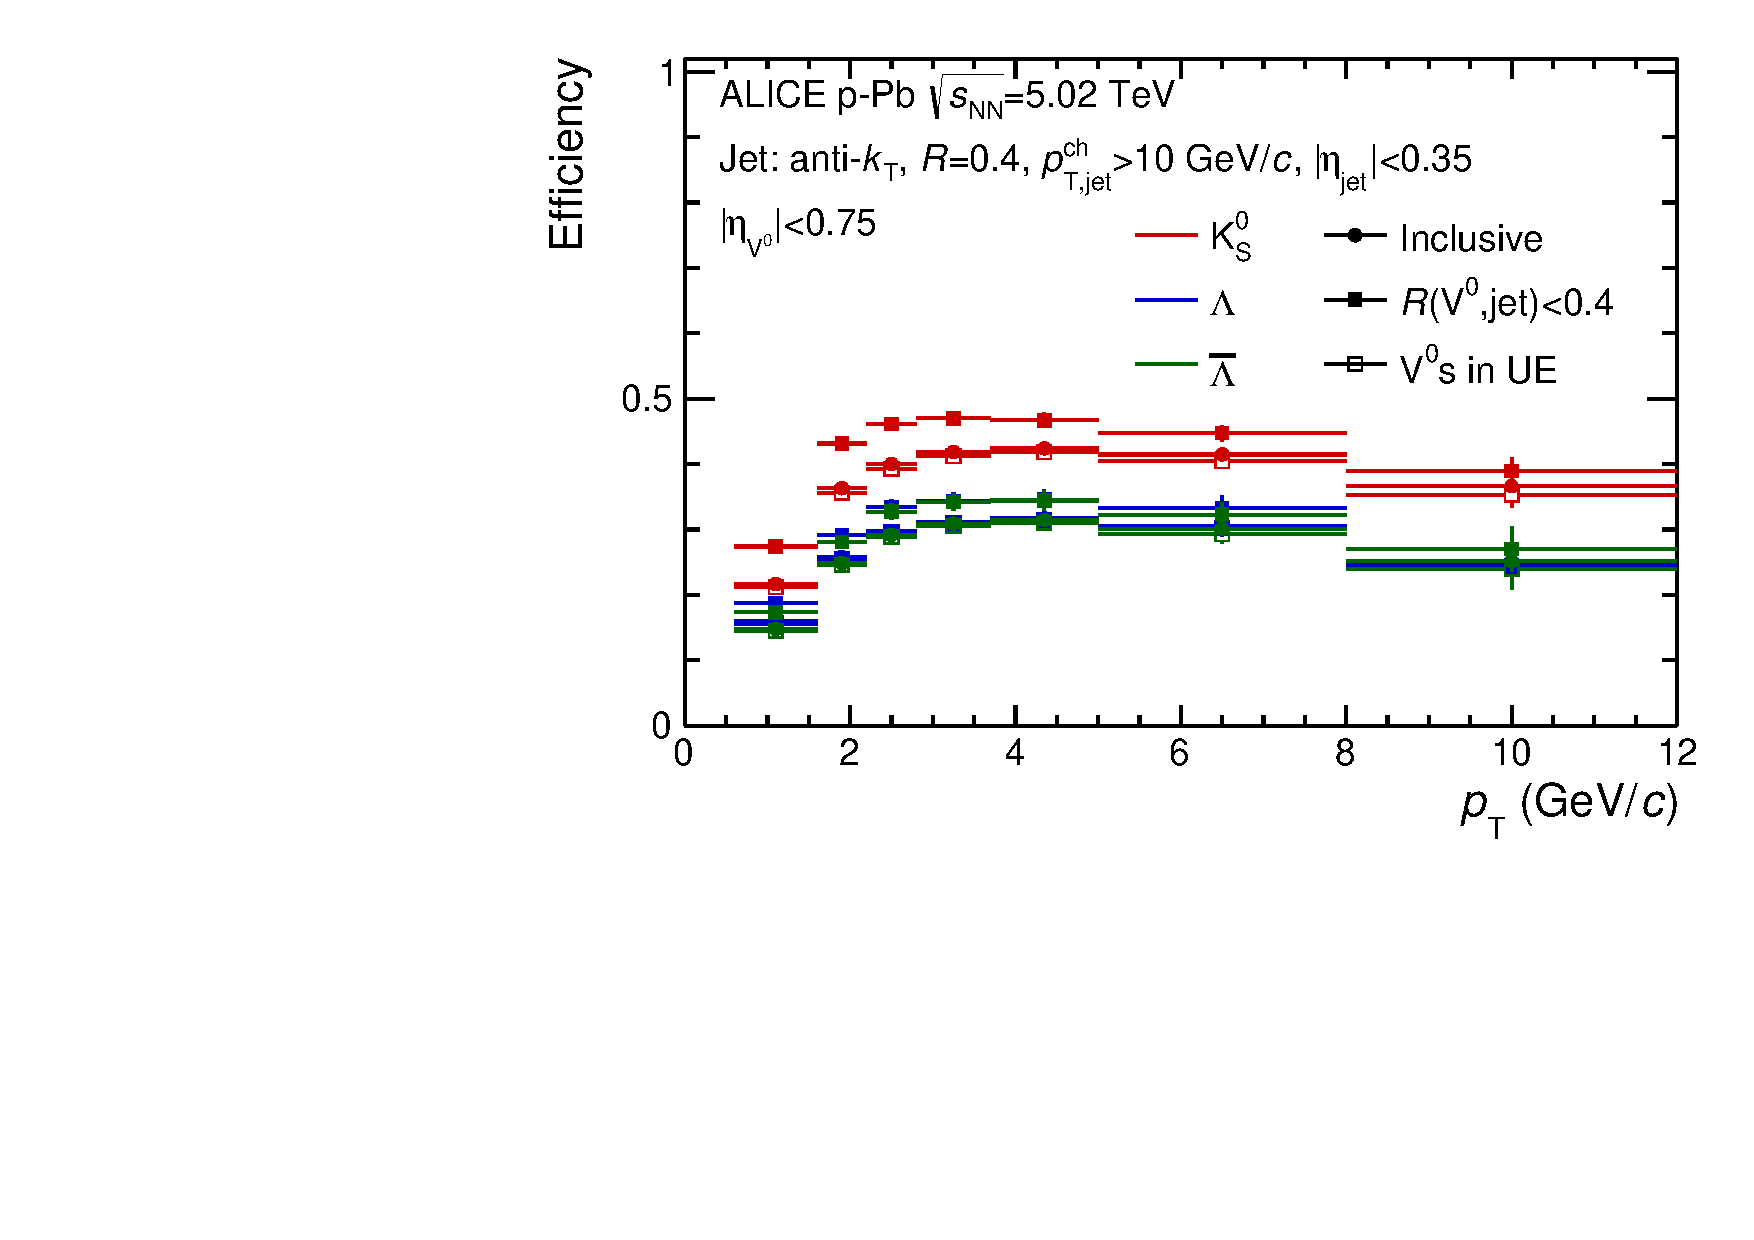
\includegraphics[width=.49\textwidth]{cFig1a_pPb}
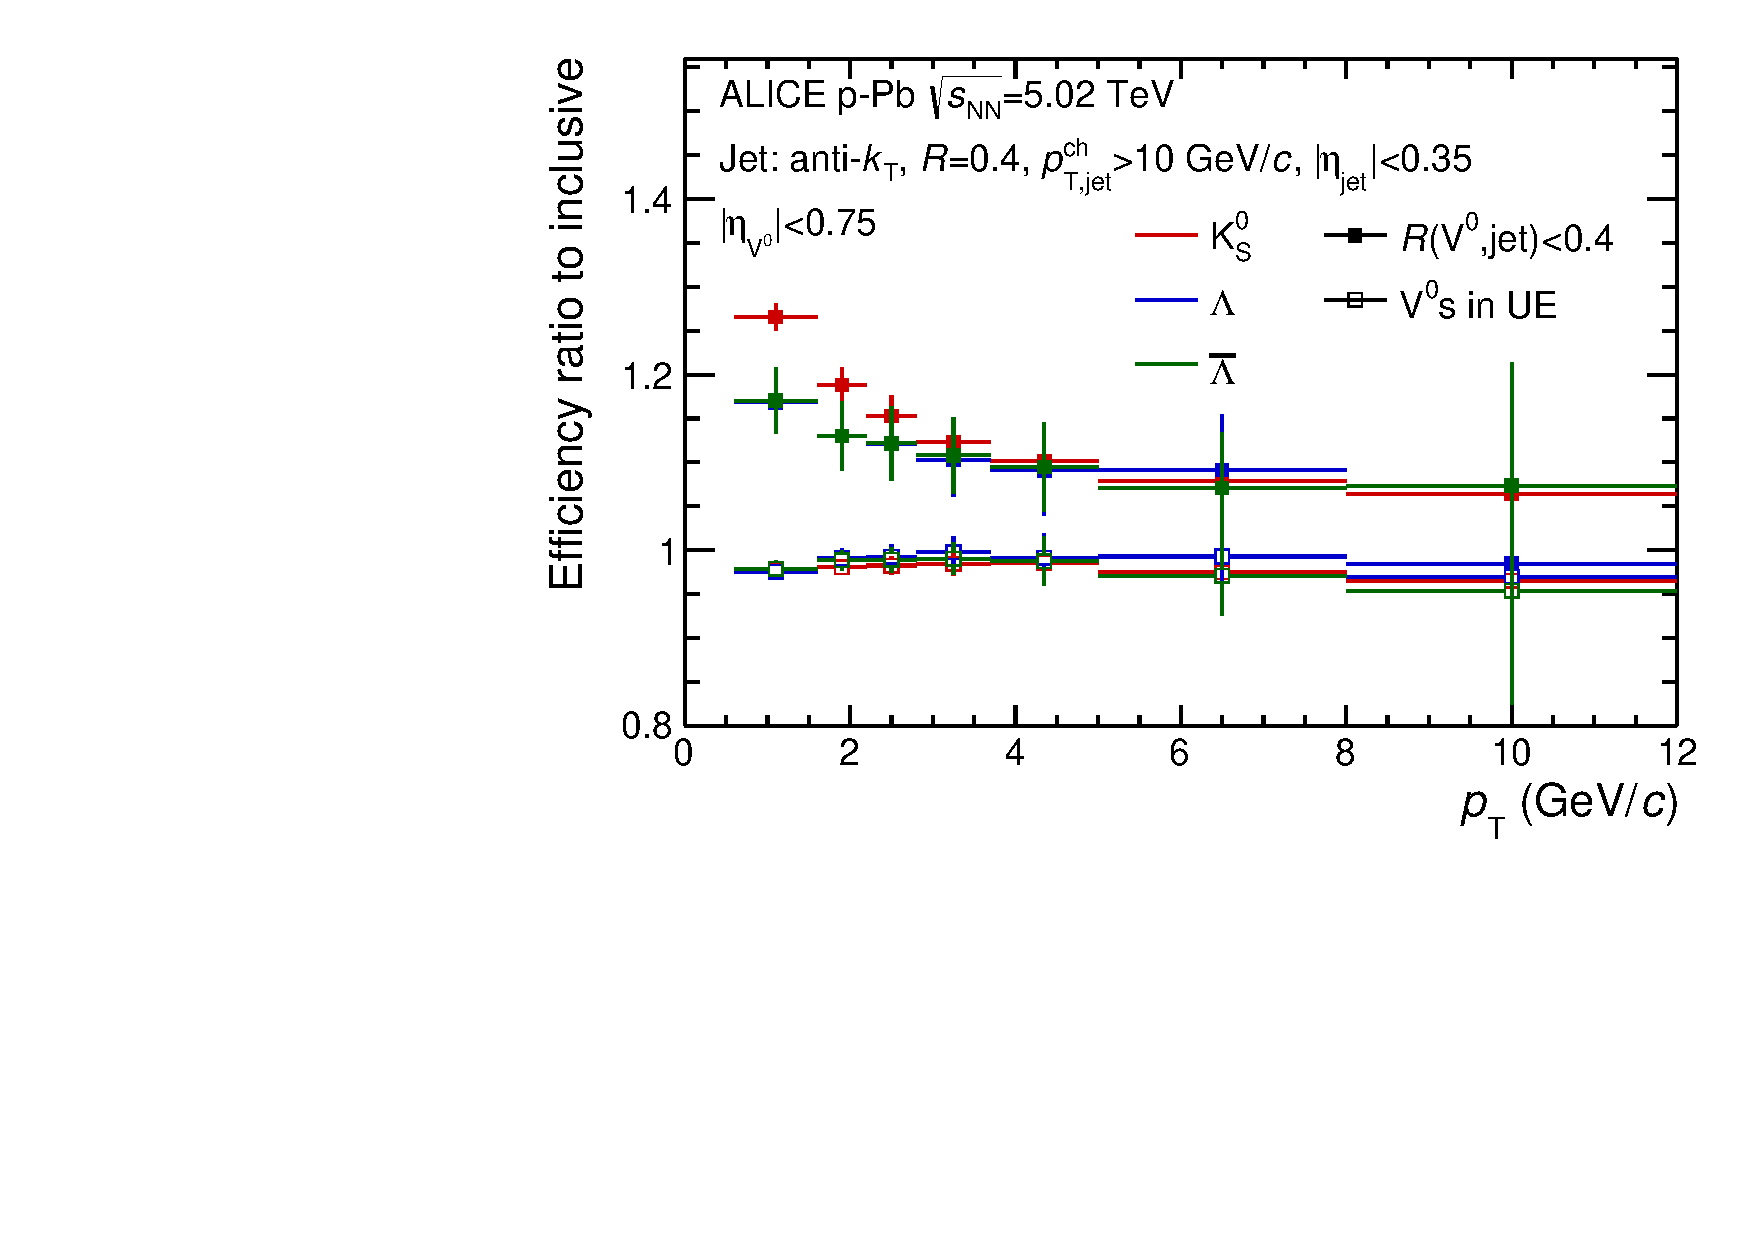
\includegraphics[width=.49\textwidth]{cFig1b_pPb} \\
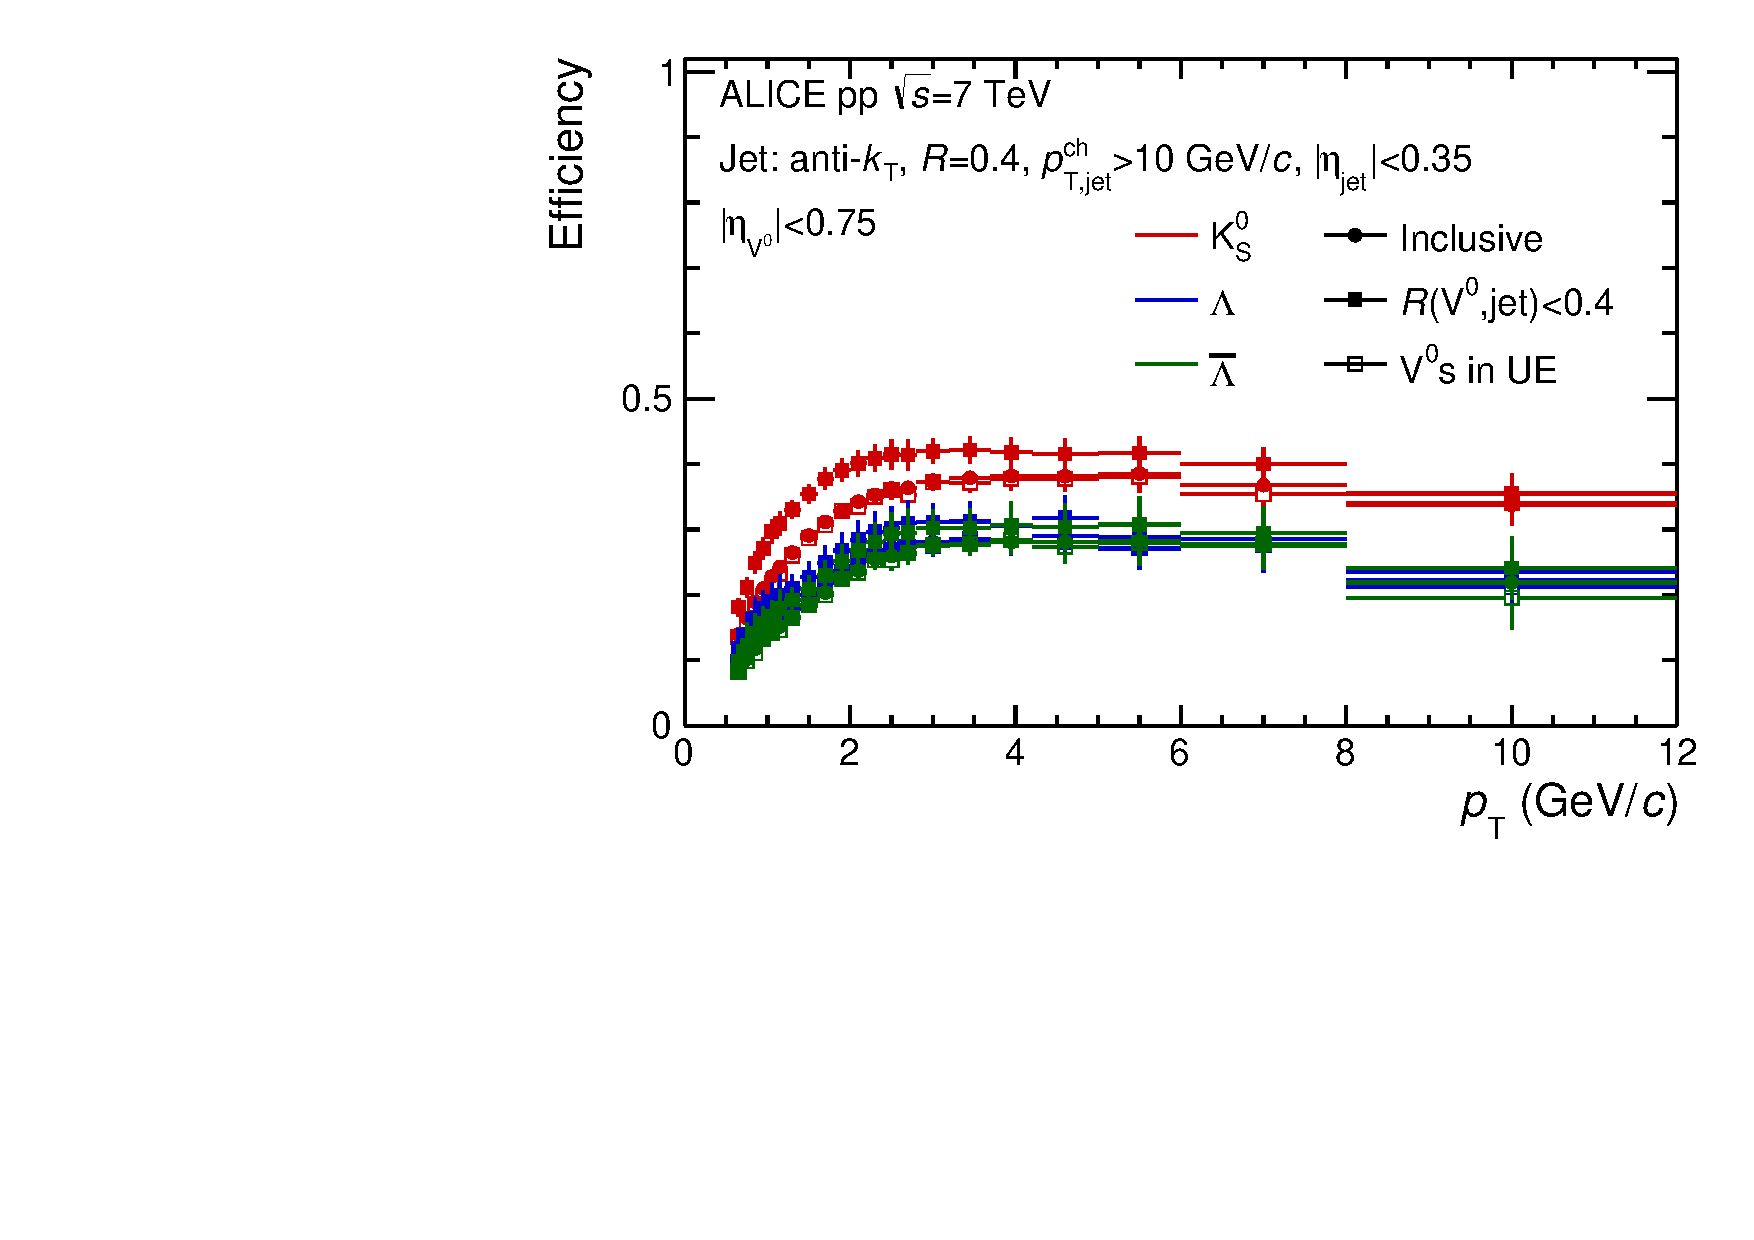
\includegraphics[width=.49\textwidth]{cFig1c_pp}
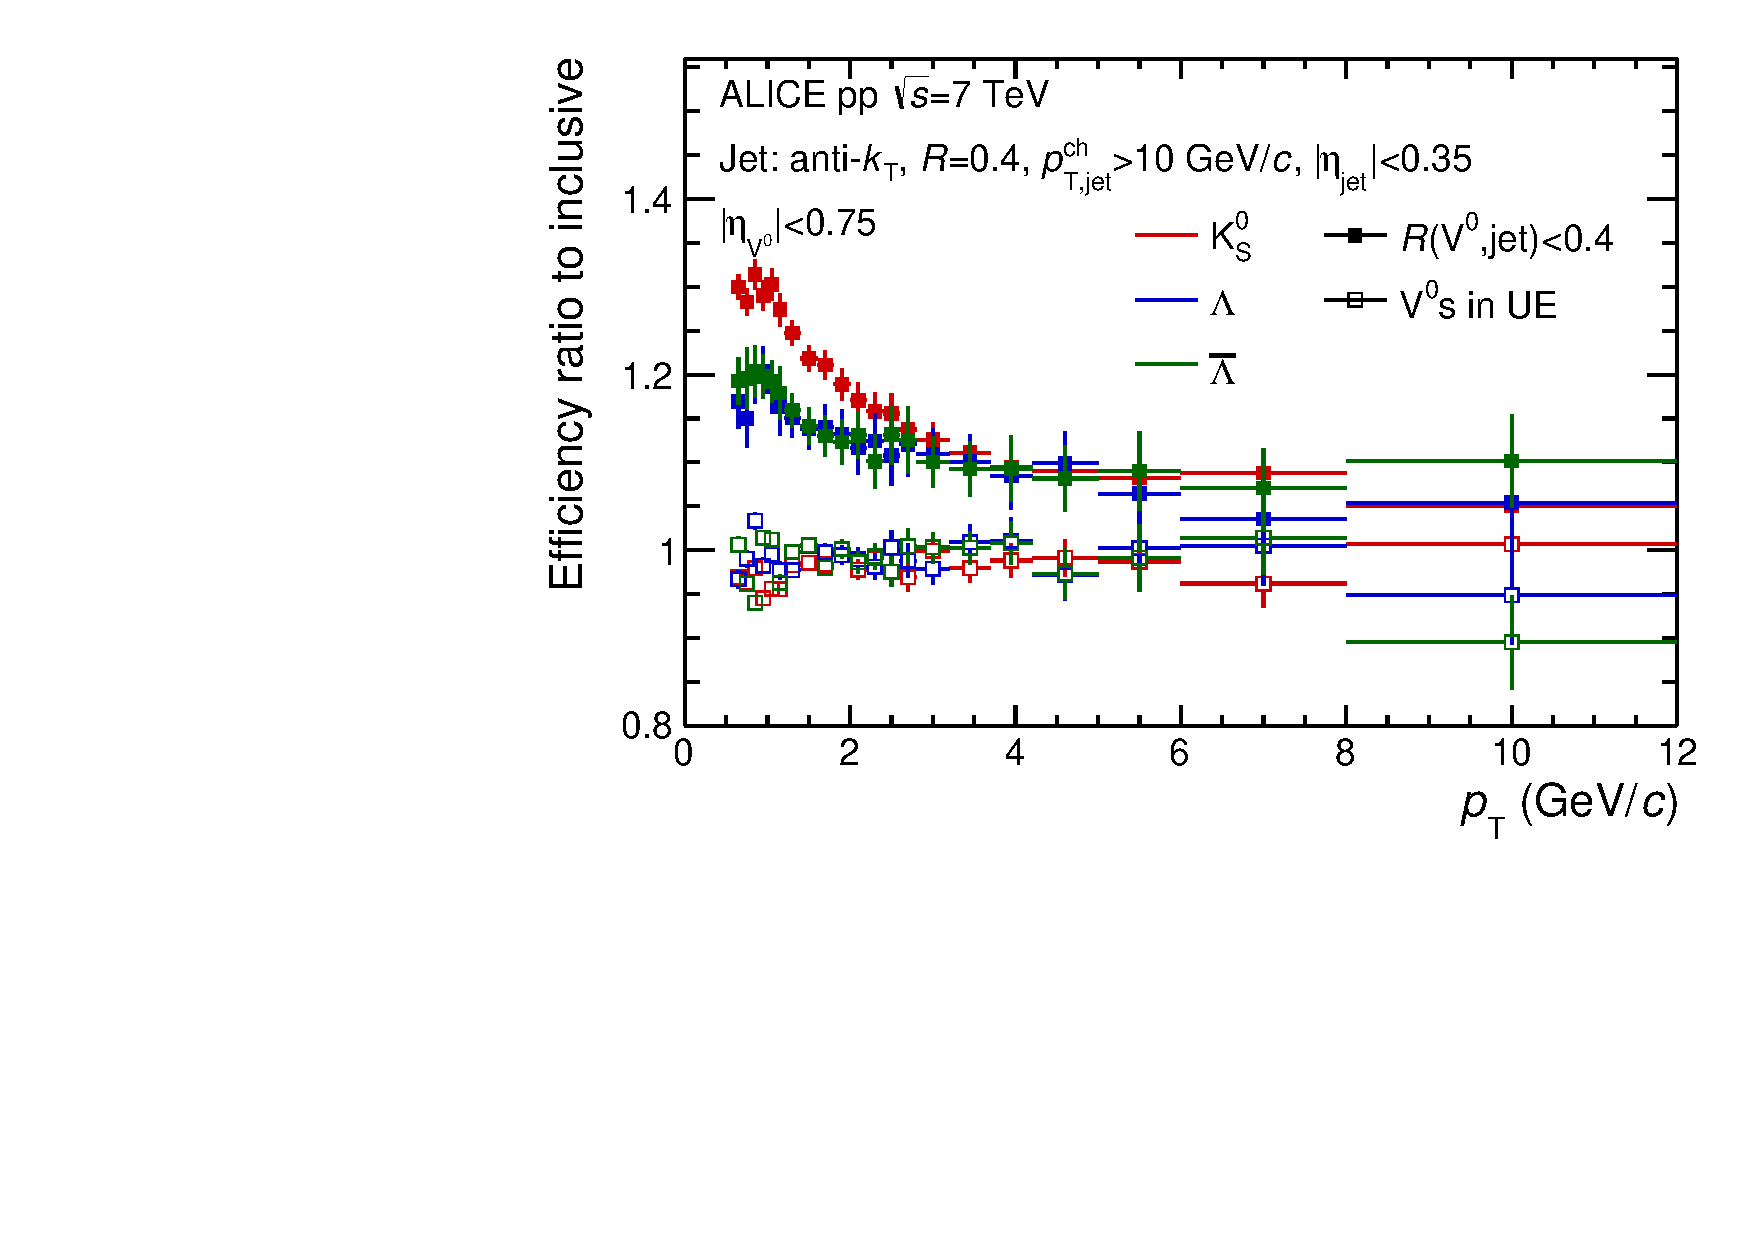
\includegraphics[width=.49\textwidth]{cFig1d_pp}
\caption{Reconstruction efficiency of \Vzero\ particles in \pPb\ collisions at \sqrtsnn{5.02} (upper pads) and in pp collisions at
$\sqrt{s}=7$~TeV (lower pads) for three selections: inclusive, within $R(\Vzero,{\rm jet})<0.4$ and $\Vzero$s in UE.
In this figure, UE $\Vzeros$ are estimated with $R(\Vzero,{\rm jet})>0.6$ in \pPb\ collisions and the PC is used as the UE estimator in pp collisions.
%The efficiency for \lda\ is consistent with the efficiency for \alda\ within about 5\% and has similar \pt\ dependence.
}
\label{fig:c02EffiIncV0s}
\end{center}
\end{figure}

Conceptually, the UE represents the particles that is not associated to the hard scatterings tagged by the charged jets considered in this analysis.
To extract the UE yield of \Vzero\ particles several estimators have been investigated: i) {\it outside cone} (OC) selection composed of the \Vzero\ particles that were not matched to any jet considered in the analysis within events containing a jet such that $R_{\Vzero-{\rm jet}} > R_{\rm cut}$ (e.g. $R_{\rm cut}=0.6$); ii) the {\it perpendicular cones} (PC) selection composed of the \Vzero\ particles found in a range with radius $R=0.4$ in $\eta$--$\varphi$ space at perpendicular direction with respect to the jet axis~\footnote{The PC is at the same eta as the jet axis}; and iii) the {\it non-jet events} (NJ) selection composed of the \Vzero\ particles found in events that do not contain a jet with $\ptjet>5~\gevc$.

In practice, a useful quantity for performing the subtraction of the non-jet contribution of the \Vzero\ particles is their density per unit area
\begin{equation}
\rho^{\Vzero}(\pt) = N^{\Vzero}(\pt) / A^{\Vzero},
\label{eq:defv0rho}
\end{equation}
where $N^{\Vzero}$ is the number of particles and $A^{\Vzero}$ is the acceptance in pseudo-rapidity and azimuthal angle. Consequently, the number of the UE \Vzero\ particles within a jet can be calculated as $N=\rho^{\Vzero} \Ajet$ for each estimator separately. In this analysis we consider the jet area $\Ajet = {\rm \pi} R^2$.
In general the density of \Vzero\ particles within jets (JC) can be defined as $\rhovzero_{\mathrm{JC}} = \rhovzero_{\mathrm{JC, raw}} - \rhovzero_{\mathrm{UE}}$, where $\mathrm{UE}$ can be any of the OC, PC, NJ background estimators.
In this analysis we choose PC as the default background estimator and use OC and NJ to quantify the systematic uncertainty.
%%%%%%%%%%%%%%%%%%%%%%%%%%%%%%%%%%%%%%%%%%%%%%%%%%%%%%%%%%%%%%%%%%

\begin{figure}[!t]
\centering
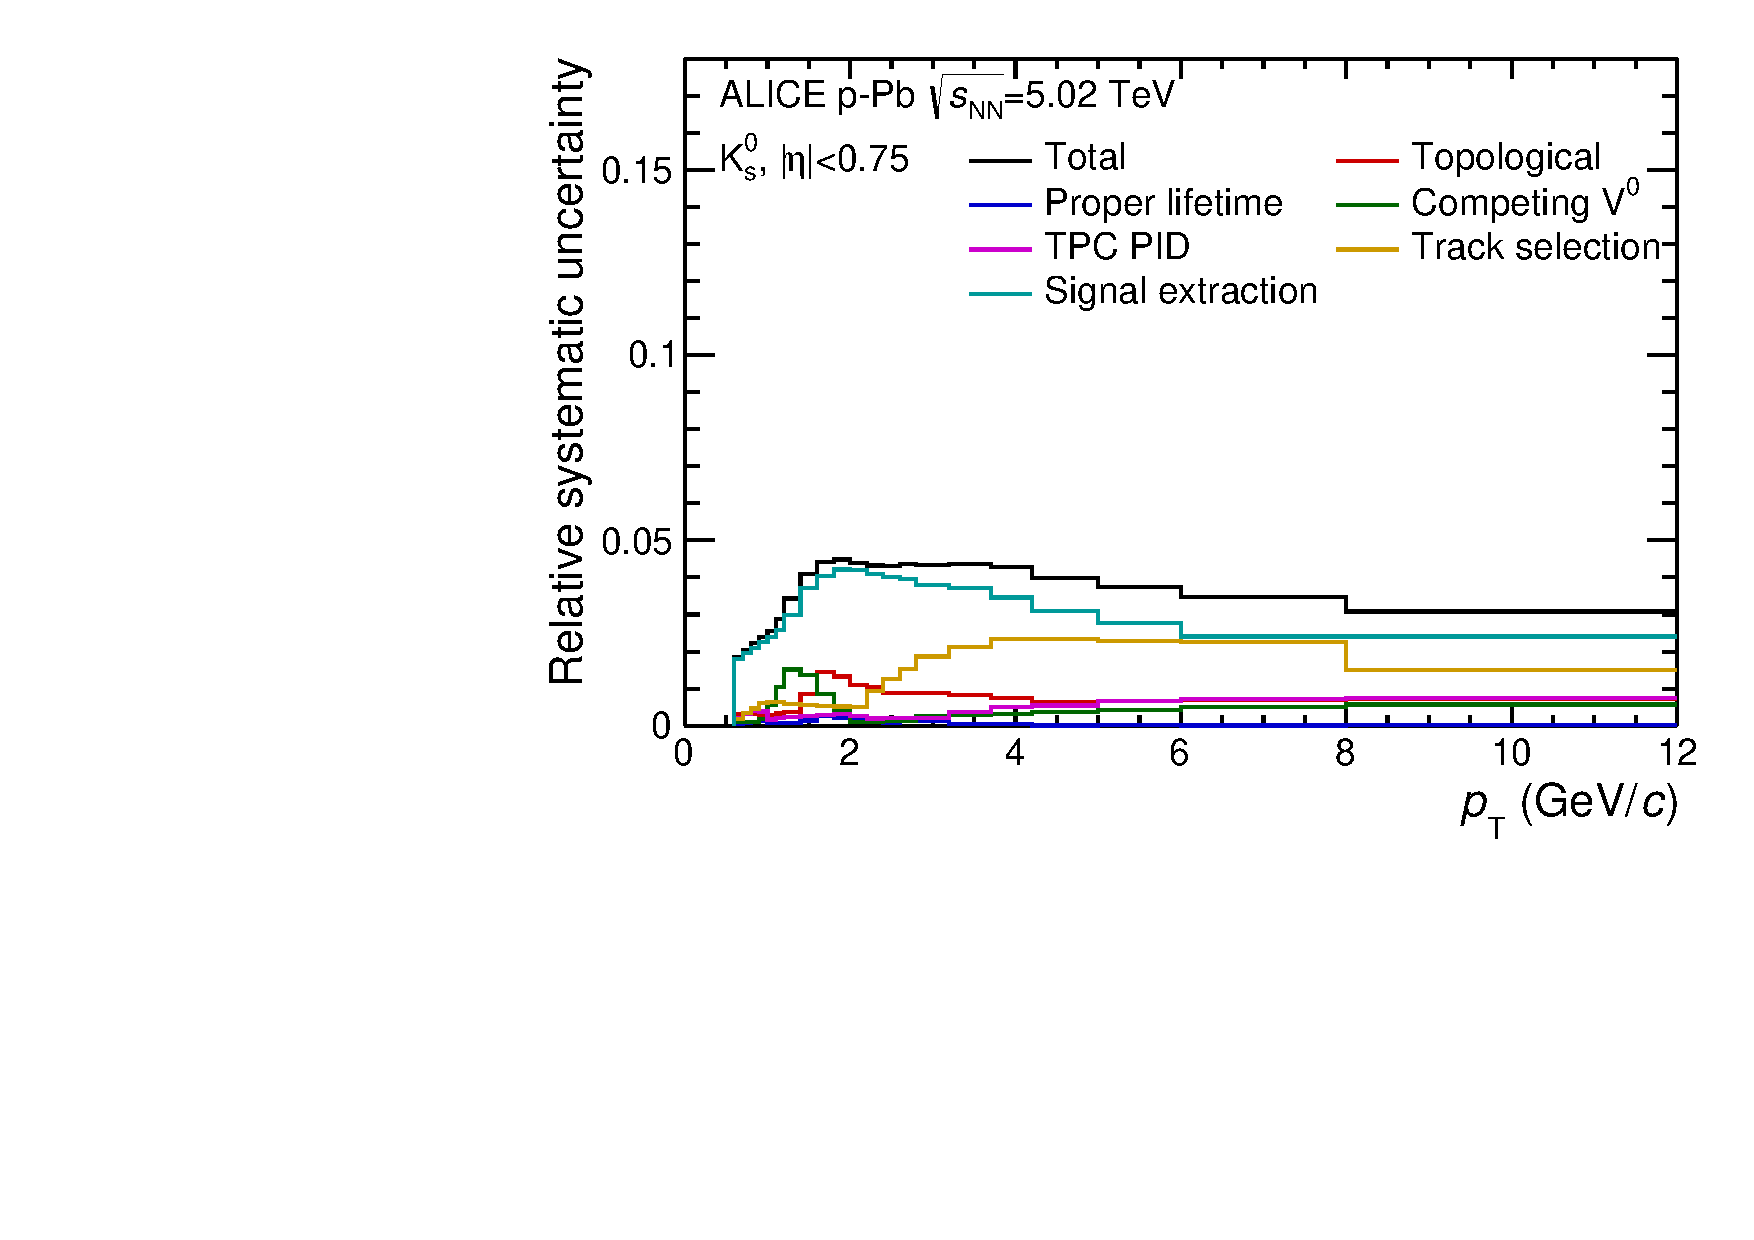
\includegraphics[width=.48\textwidth]{cFig2a_pPb}
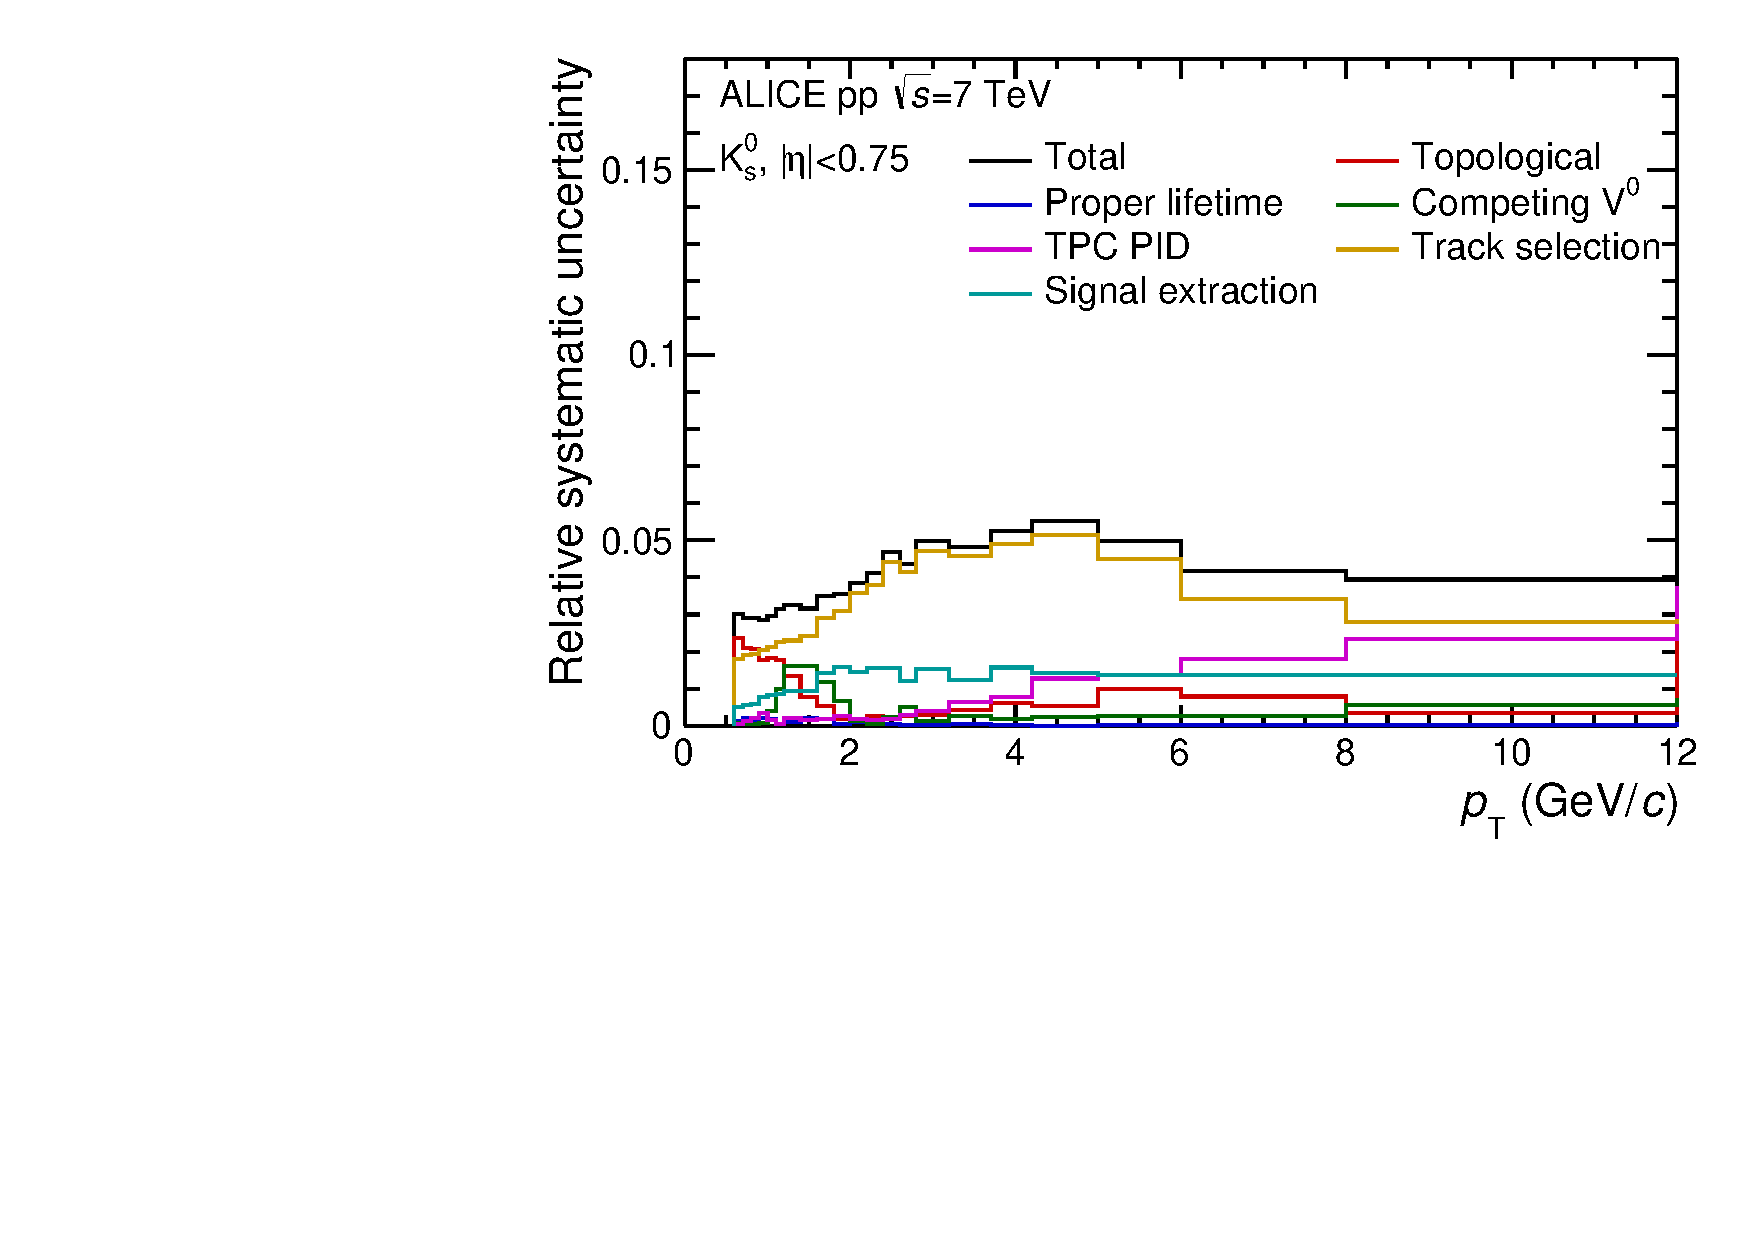
\includegraphics[width=.48\textwidth]{cFig2c_pp} \\
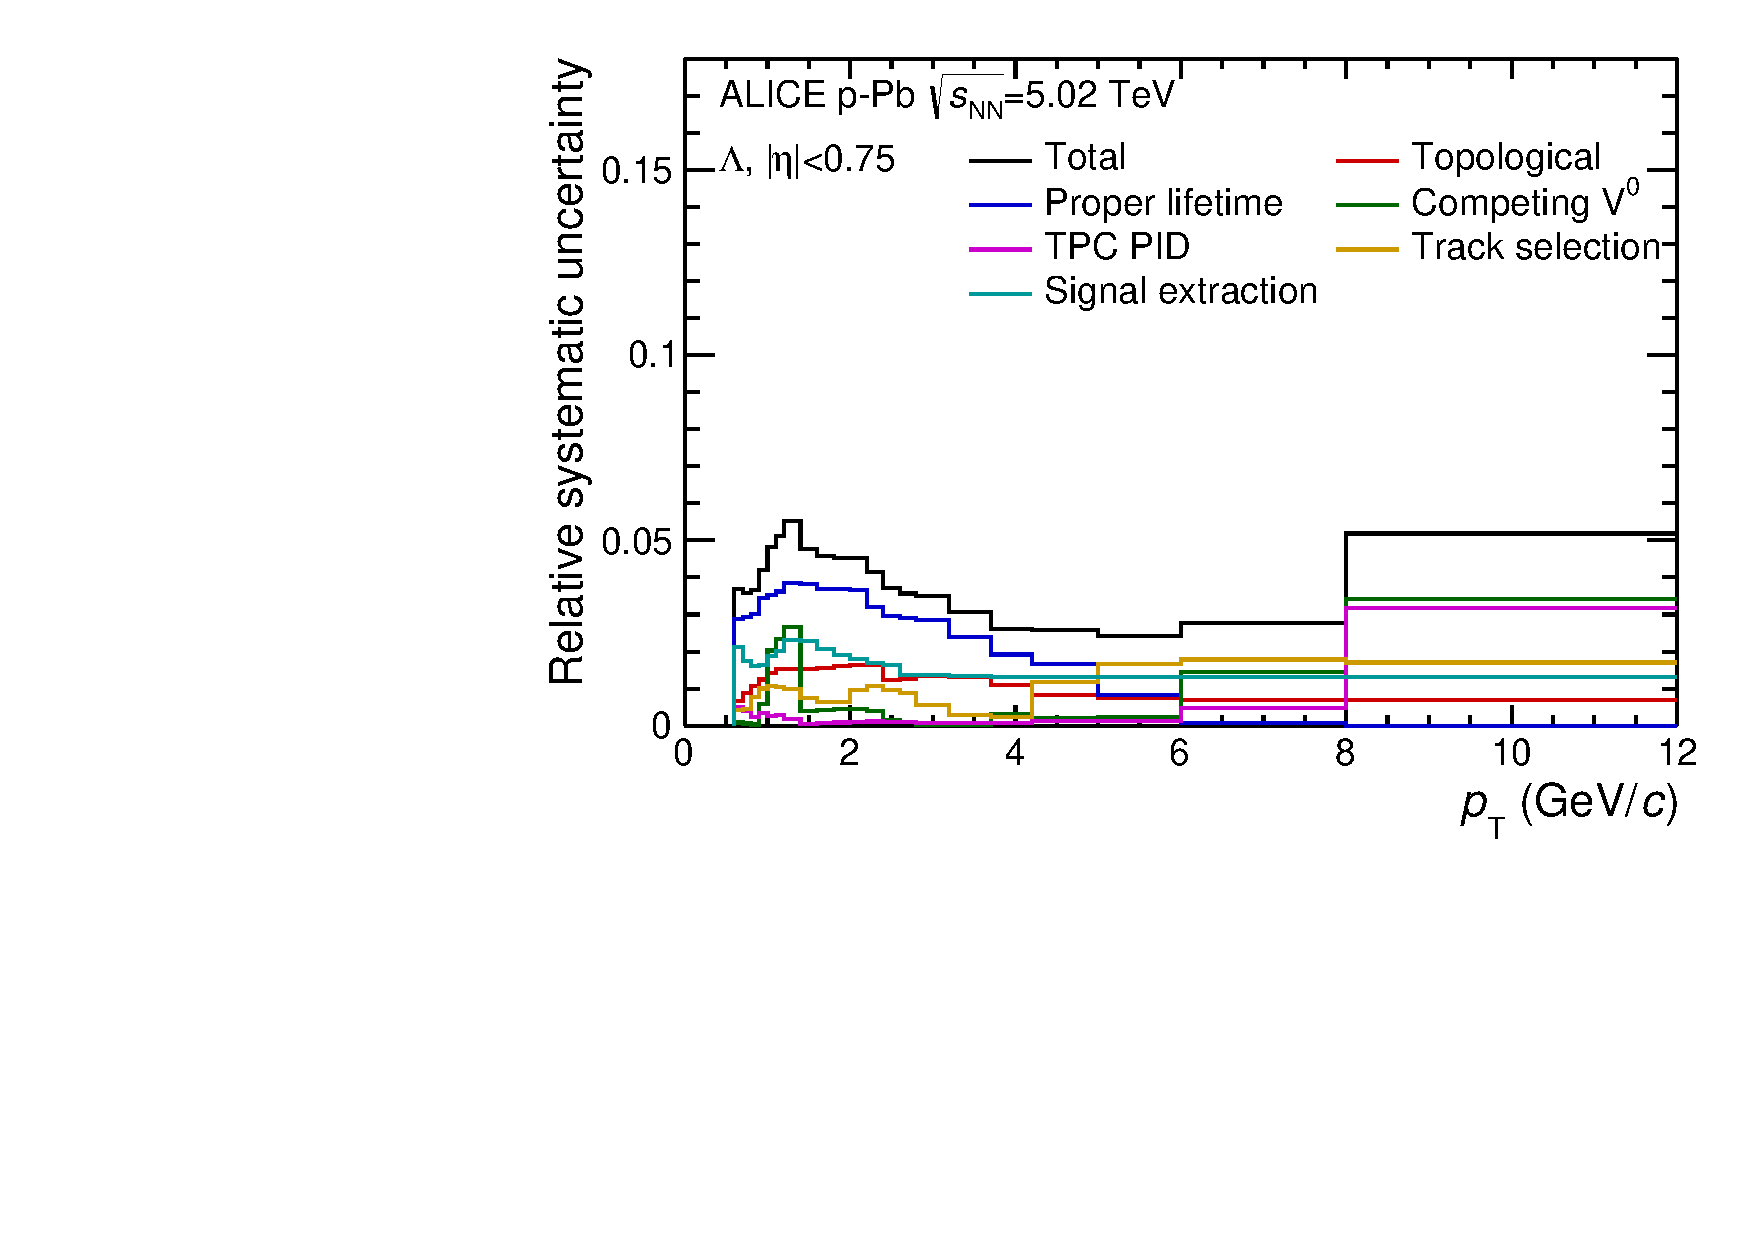
\includegraphics[width=.48\textwidth]{cFig2b_pPb_Lambda}
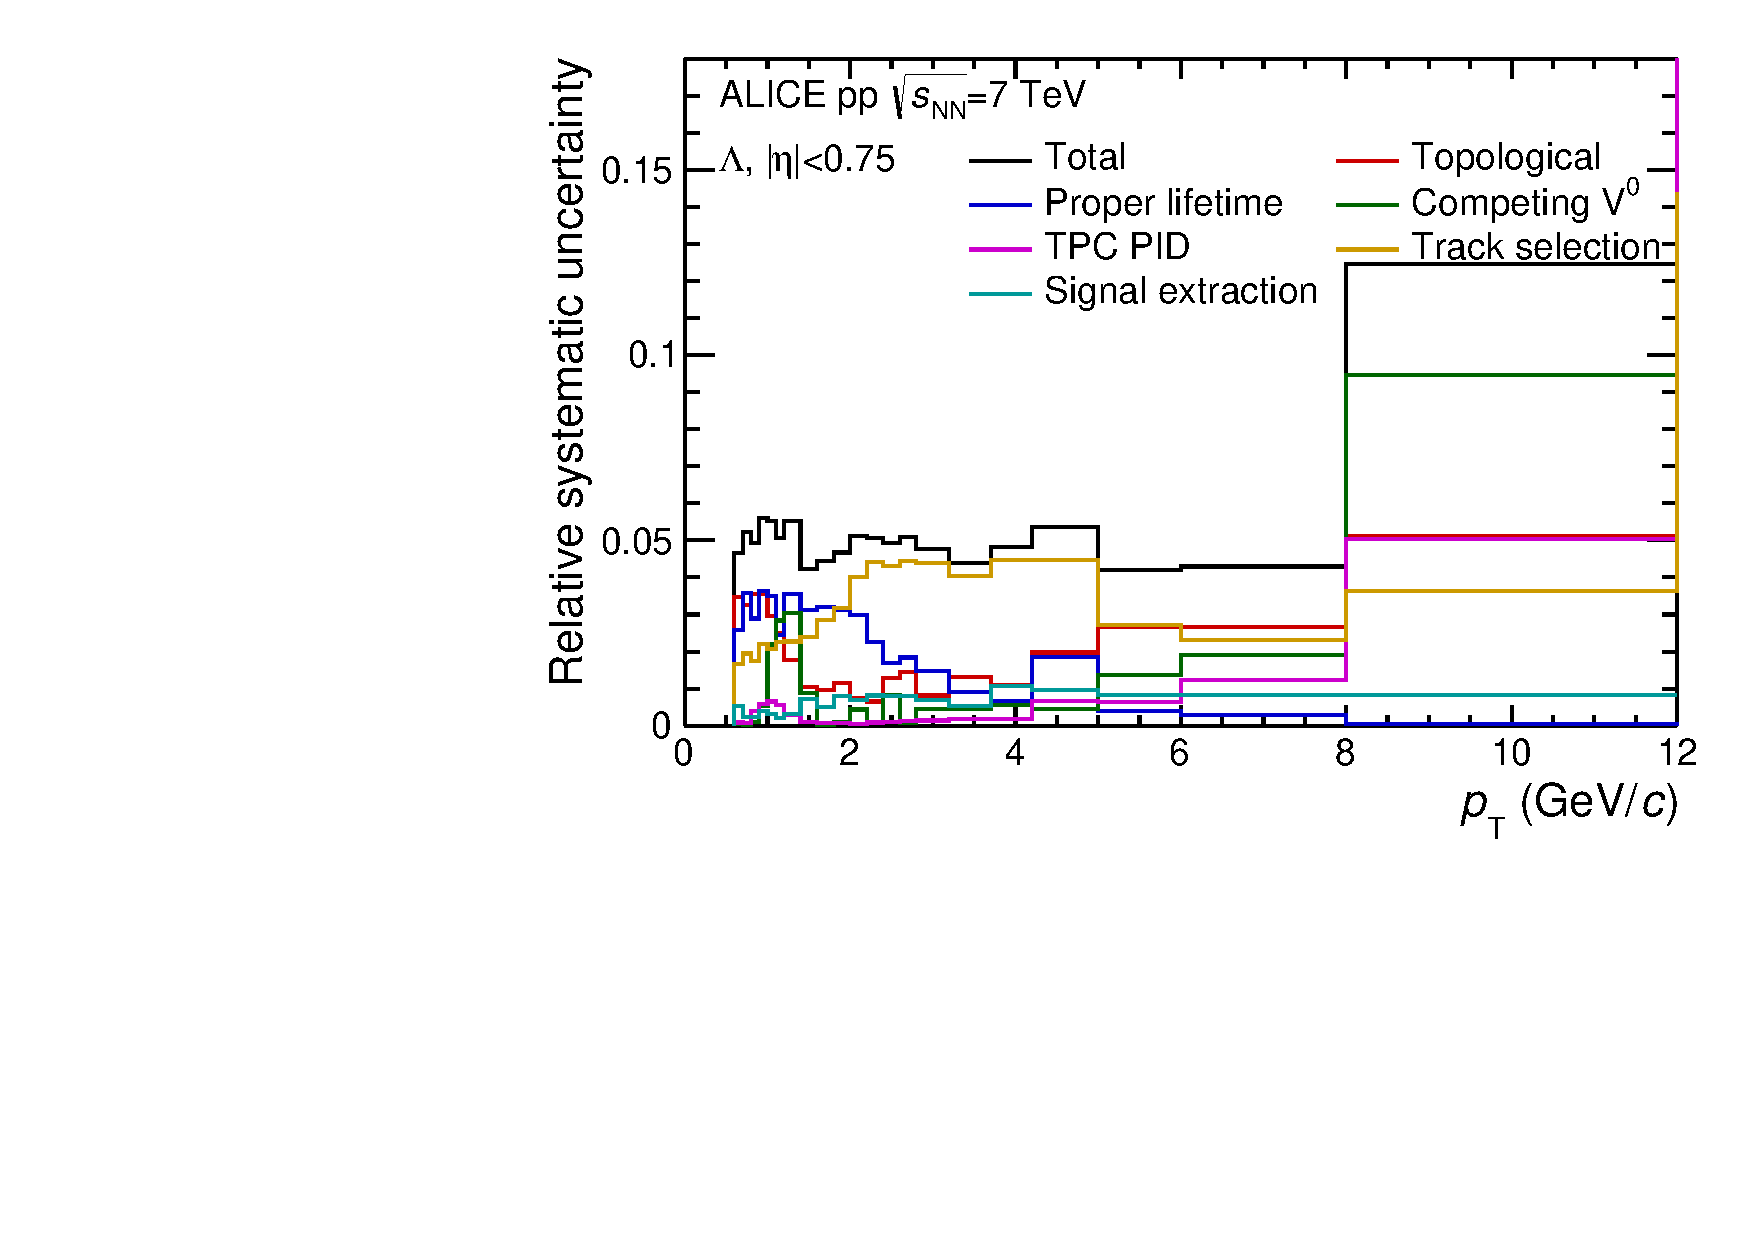
\includegraphics[width=.48\textwidth]{cFig2d_pp_Lambda} \\
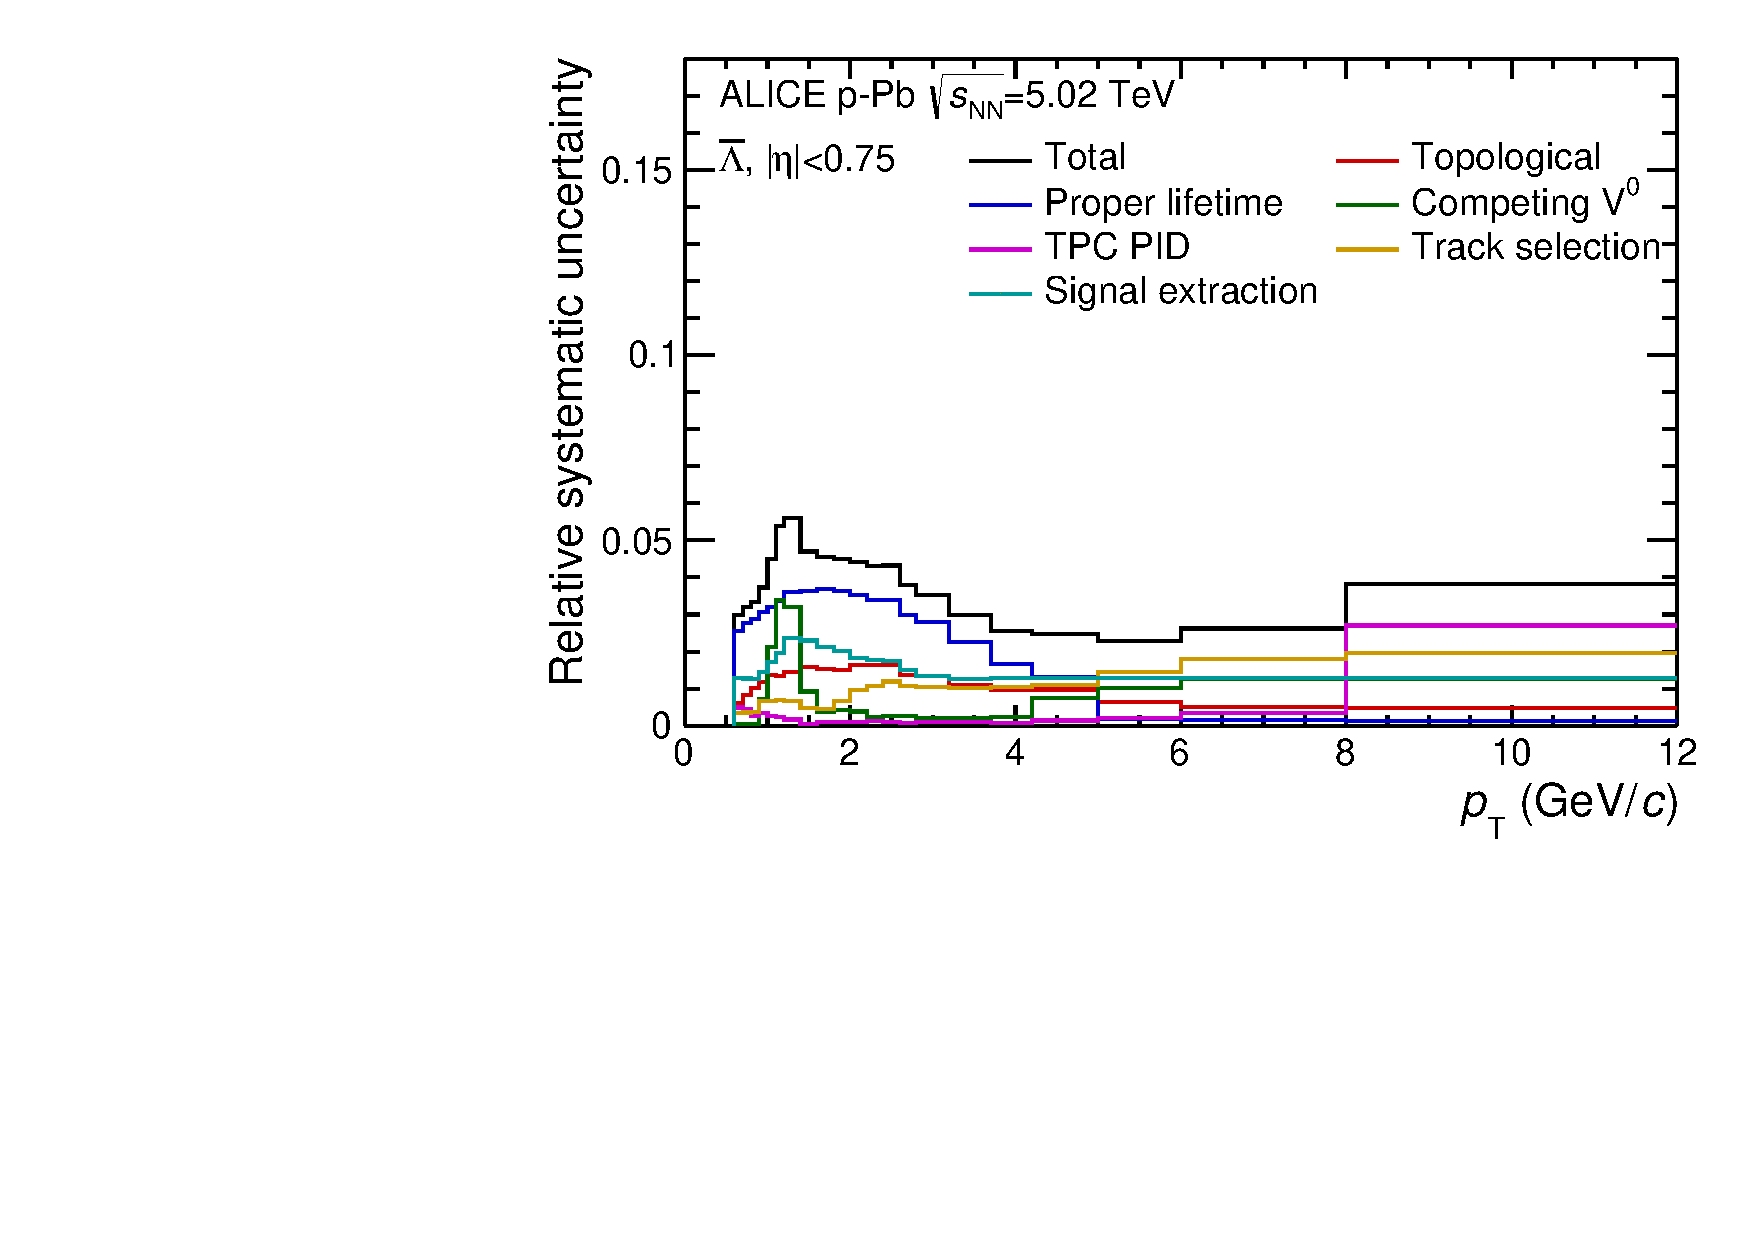
\includegraphics[width=.48\textwidth]{cFig2b_pPb_AntiLa}
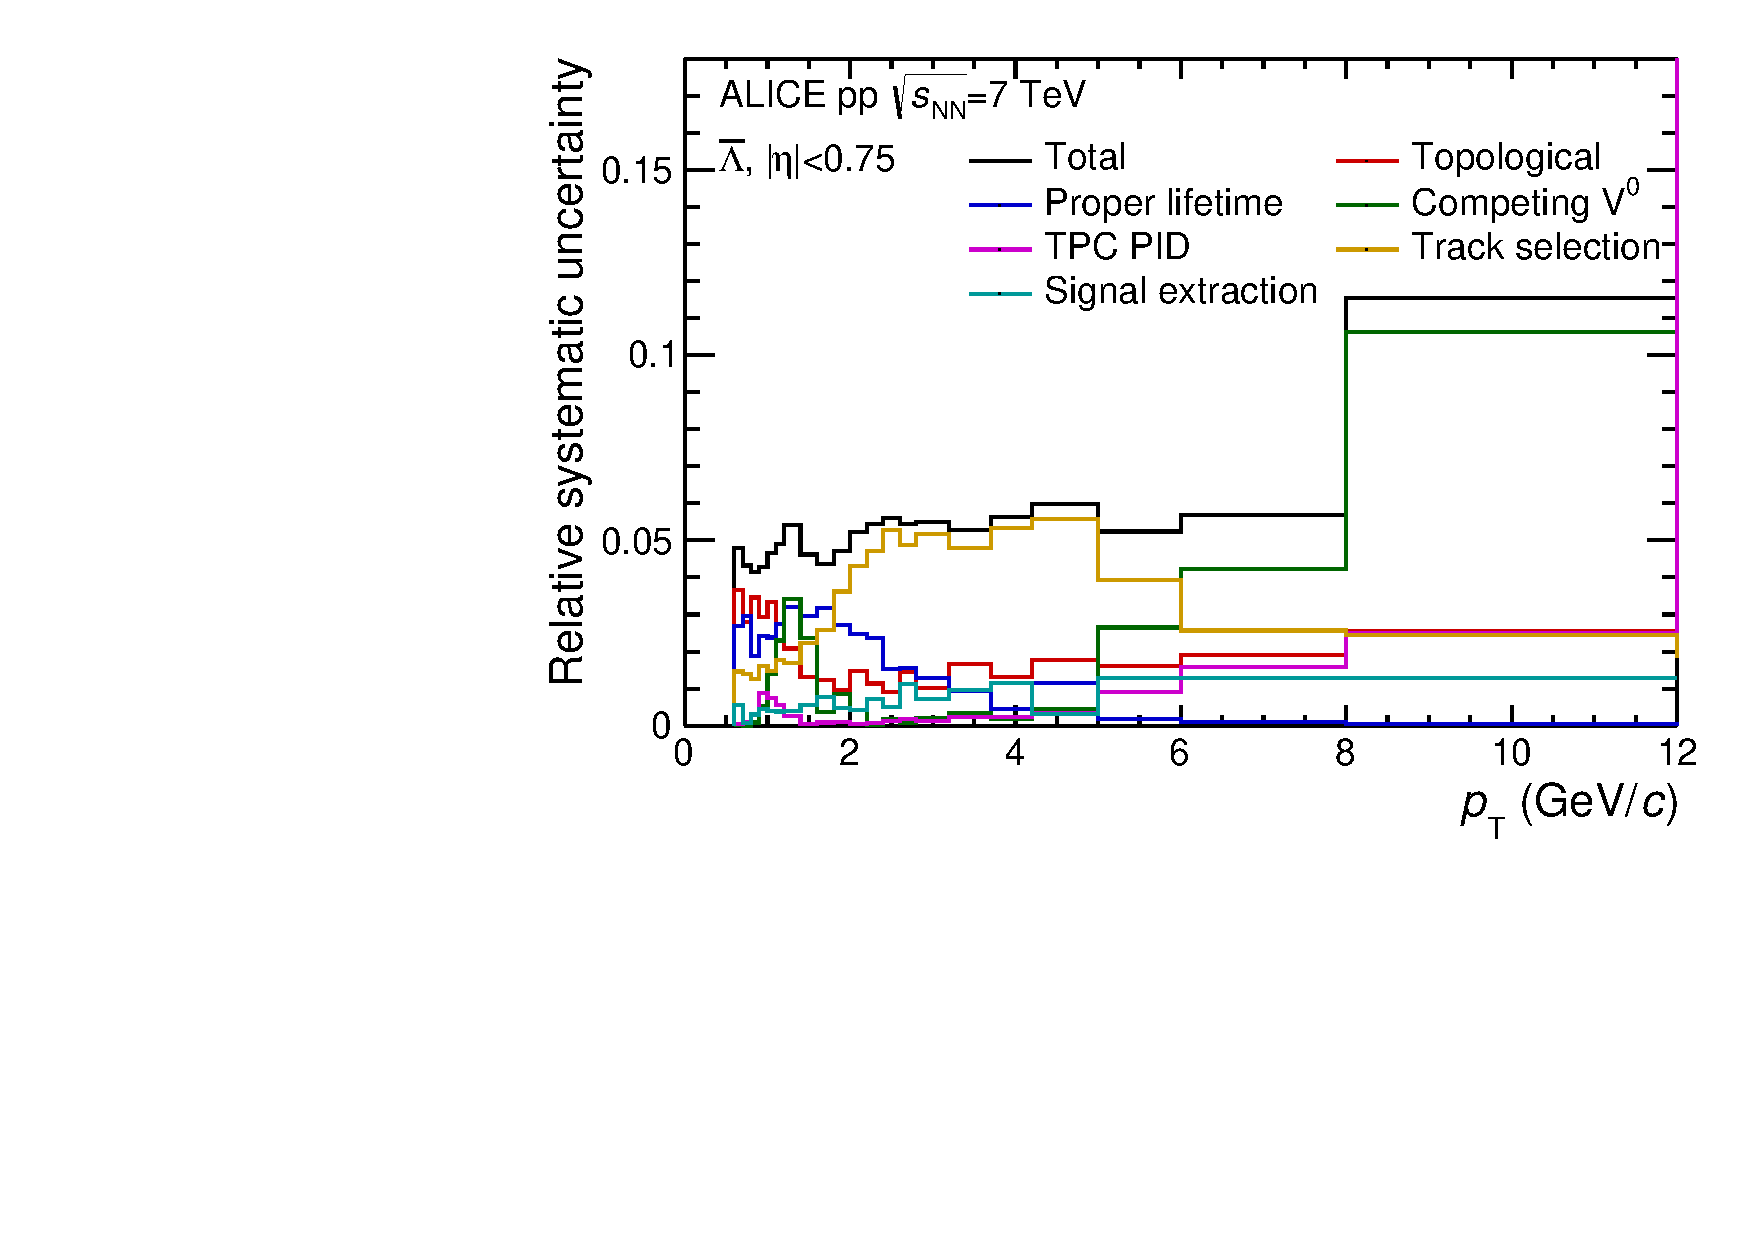
\includegraphics[width=.48\textwidth]{cFig2d_pp_AntiLa} \\
\caption{Relative systematic uncertainties on transverse momentum spectra of \ks\ (upper), \lda\ (middle) and \alda\ (lower) in \pPb\ collisions at \sqrtsnn{5.02} (left) and pp collisions at \sqrts{7} (right), see text for details.}
	\label{fig:systUncert}
\end{figure}

\begin{figure}[!ht]
	\centering
	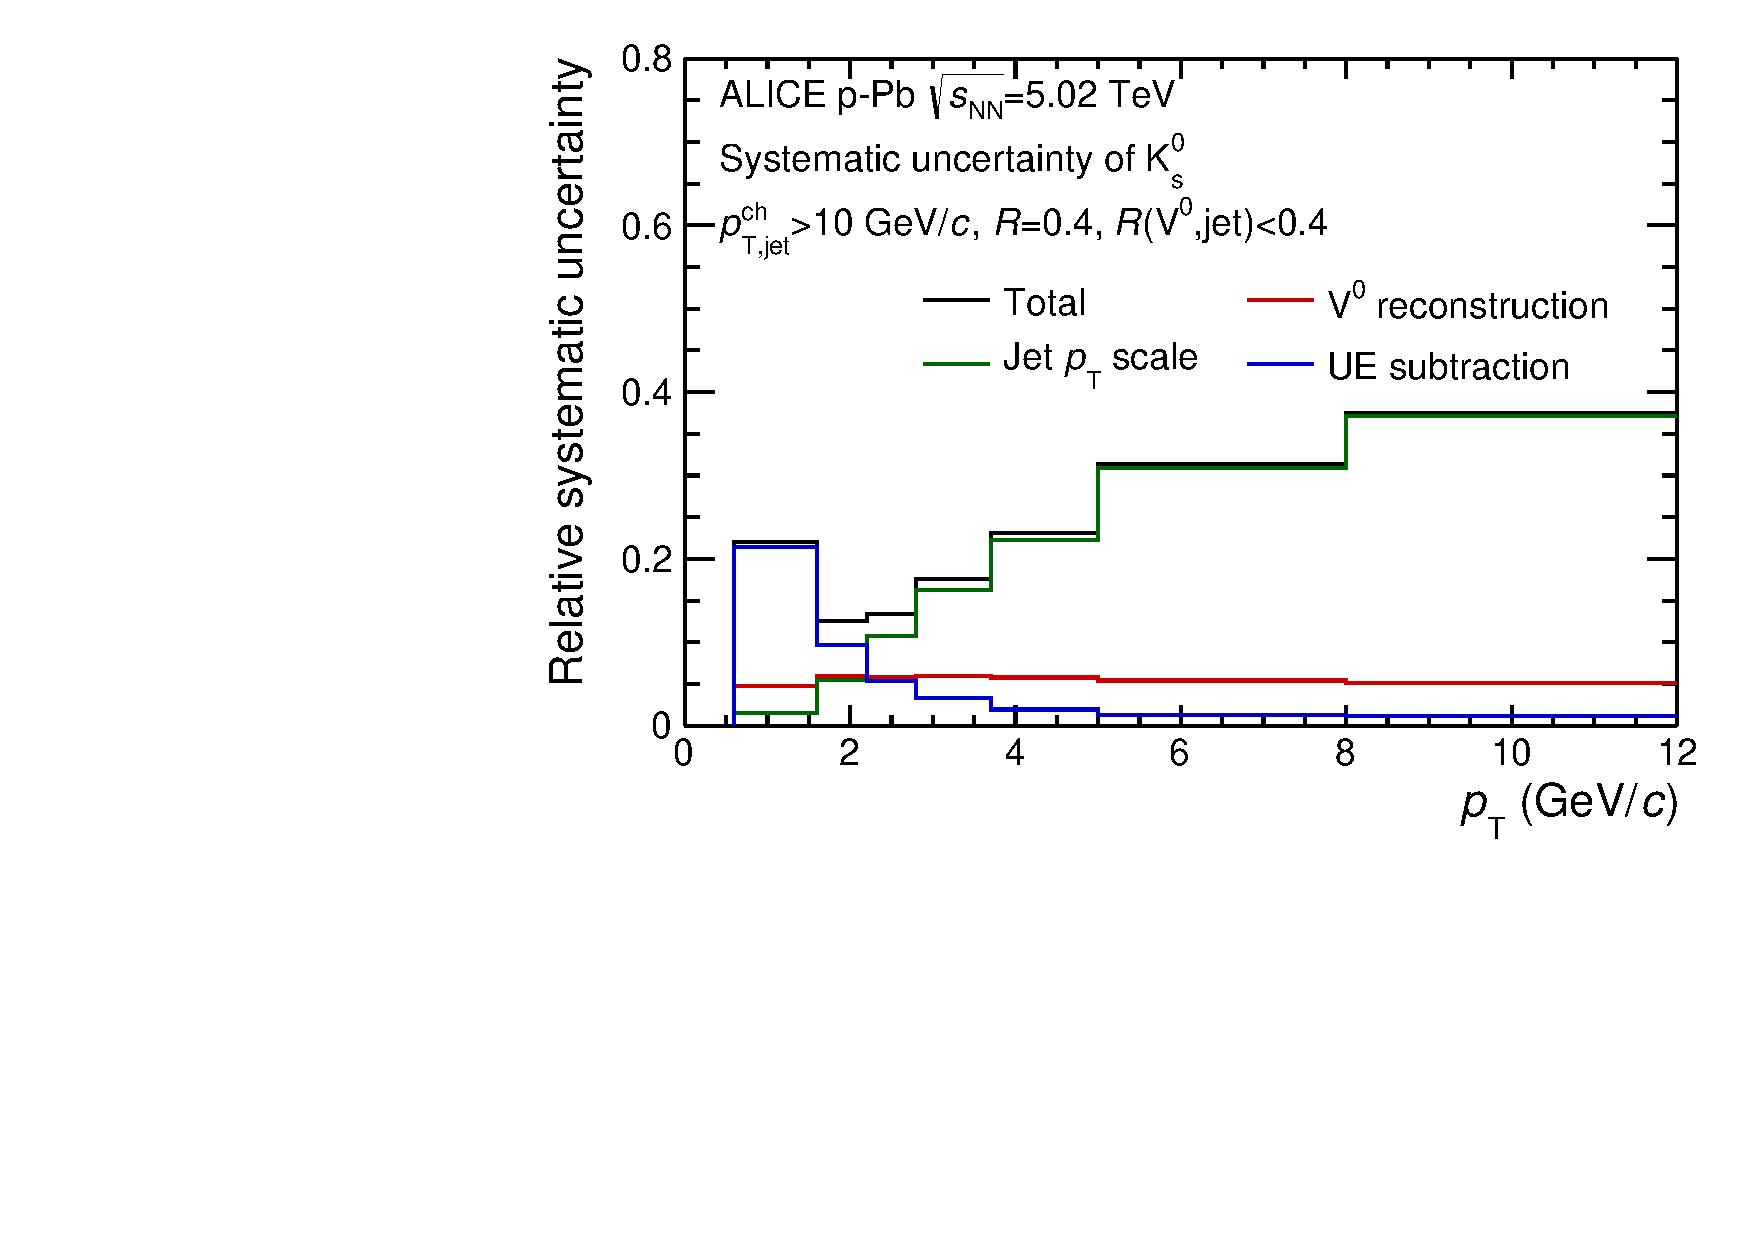
\includegraphics[width=.49\textwidth]{cFig3a_pPb}
        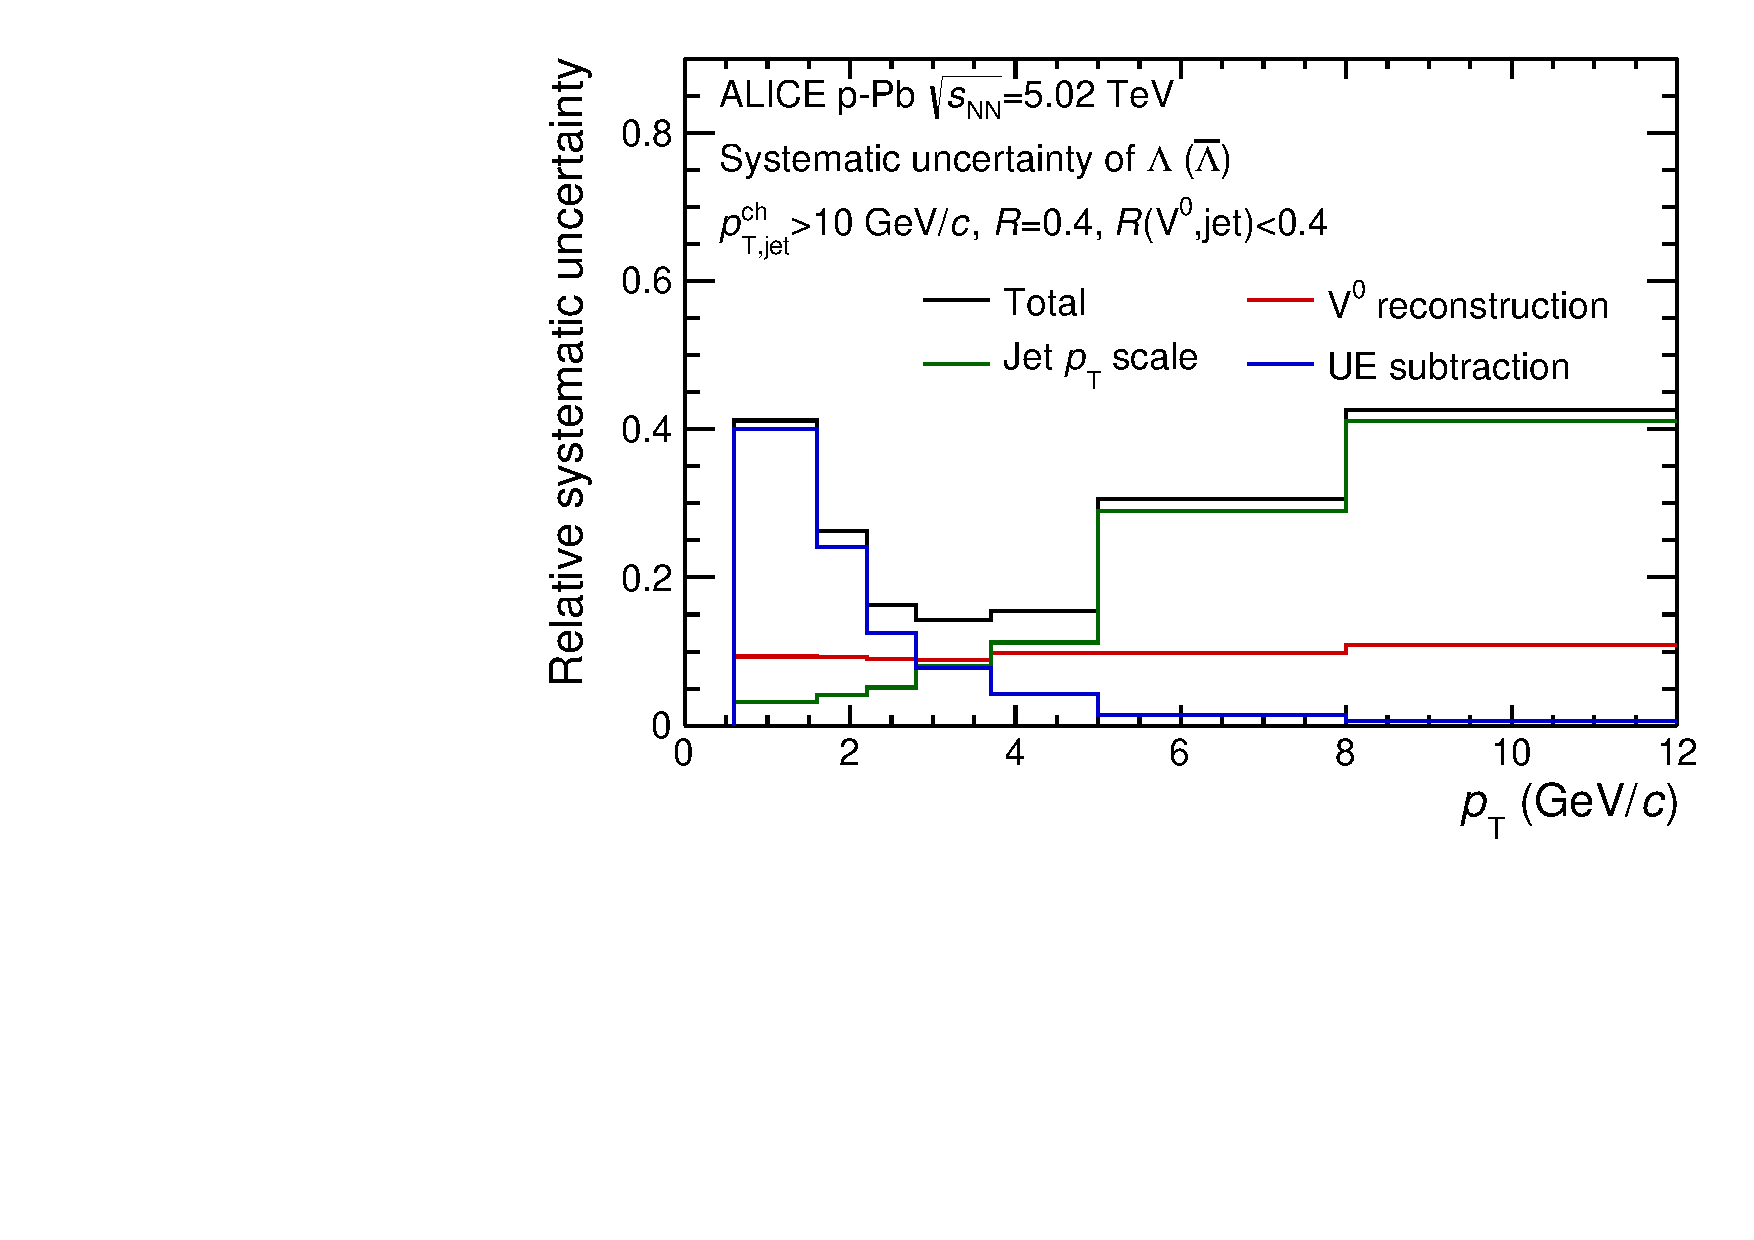
\includegraphics[width=.49\textwidth]{cFig3b_pPb} \\
        	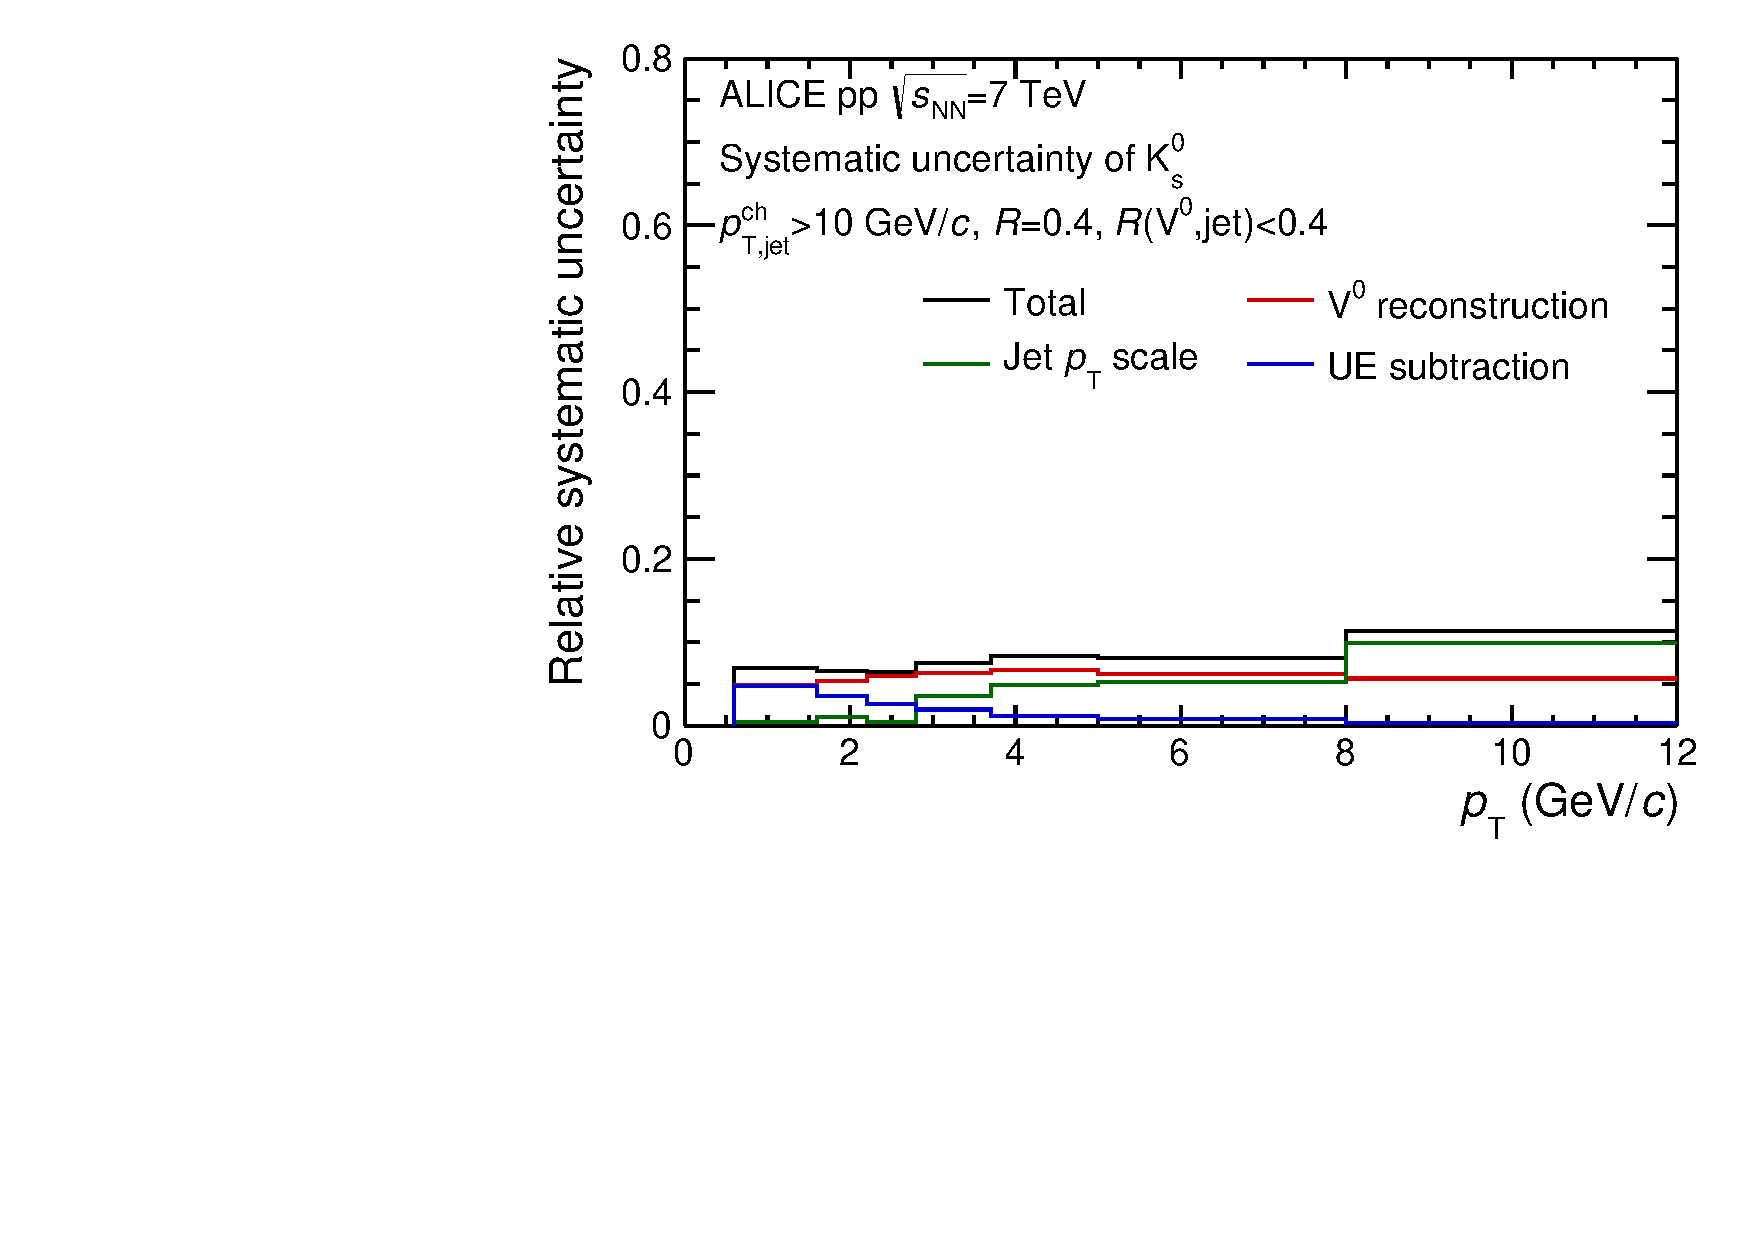
\includegraphics[width=.49\textwidth]{cFig3c_pp}
        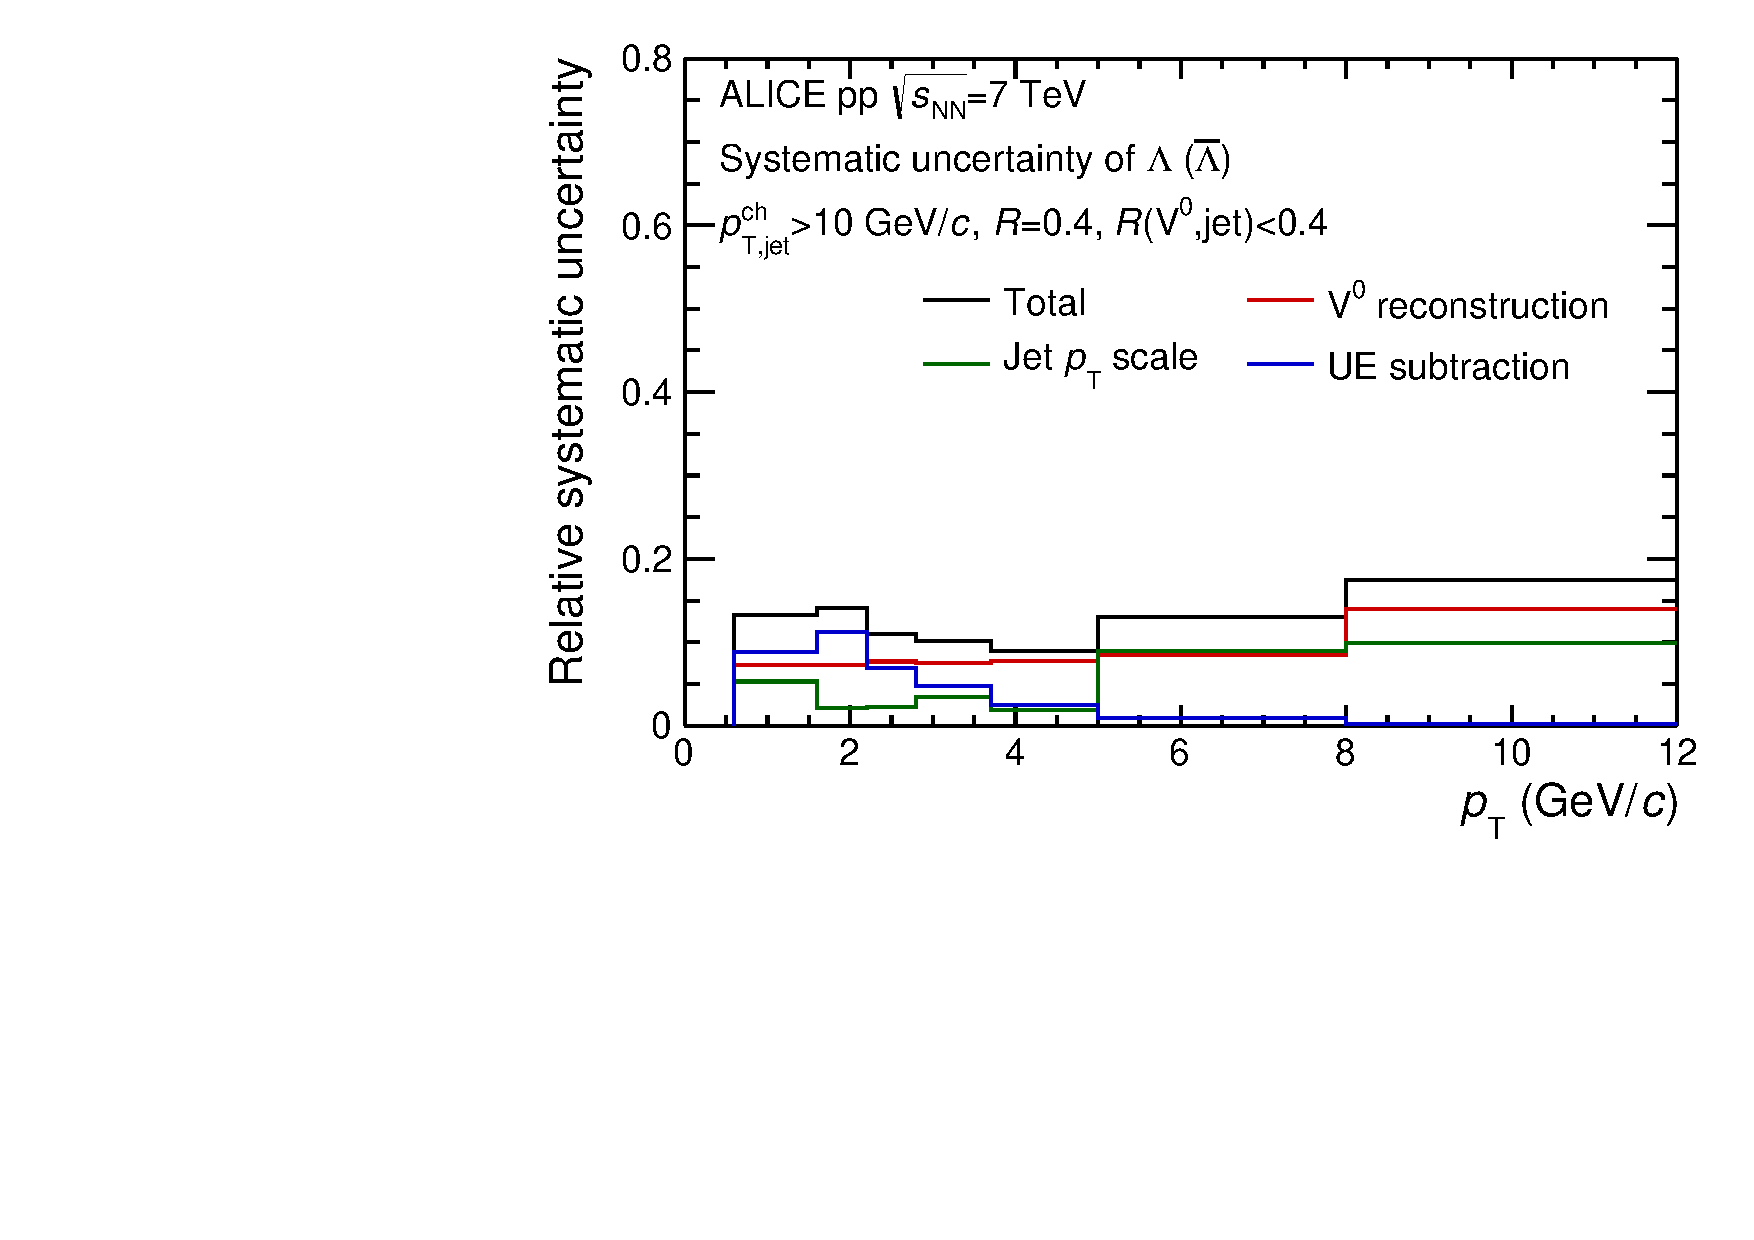
\includegraphics[width=.49\textwidth]{cFig3d_pp}
	\caption{Relative systematic uncertainties on \Vzero\ particle spectrum \ks, \lda\ and \alda\ produced in jets as a function of their transverse momentum (see text for details) in p--Pb collisions at $\snn=5.02$~TeV (upper) and \pp\ collisions at \sqrts{7} (lower). The uncertainties for \lda\ and \alda\ are combined in the plots. The red curves in each plot correspond to the total uncertainty on \Vzero\ yield extraction (shown in Fig.~\ref{fig:systUncert}).}
	\label{fig:systUncert_pp}
\end{figure}

\subsection{Corrections for finite \Vzero\ reconstruction efficiency and feed-down}
\label{sec:c05V0EffiMC}

The reconstruction efficiencies of \Vzero\ particles were estimated using, respectively, DPMJET~\cite{Roesler:2000he} and \textsc{Pythia} Monte Carlo generators in p--Pb and pp collisions with the same cuts as in the data except the daughter track particle identification with ${\rm d}E/{\rm d}x$ in TPC (see more details in \cite{Abelev:2013haa}).
These simulations are based on the GEANT3 transport code~\cite{Brun:1994aa} for the detector description and response.
The time evolution of detector configuration is considered.

Due to differences in the experimental acceptance for \Vzero\ particles associated to jets (JC) and those extracted through the various estimators of the underlying event (OC, PC, NJ) the efficiencies of \Vzero\ particles were estimated separately for every case. Figure~\ref{fig:c02EffiIncV0s} shows the inclusive reconstruction efficiency for $\Vzero$ particles and the efficiency in the events containing a jet for two selections of distance $R$ from the main jet axis. In particular, for $\rvzerojet<0.4$ the efficiency at $\pt<2~\gevc$ is about 20\% greater than in the inclusive case while it approaches the inclusive case at higher $\pt$. The efficiency for events containing a jet varies moderately with $R$ (within a 5\%) and for every selection of $R$ the efficiencies were evaluated separately.
%%%%%%%%%%%%%%%%%%%%%%%%%%%%%%%%%%%%%%%%%%%%%%%%%%%%%%%%%%%%%%%%%%

The \pt\ differential yields of \lda\ and \alda\ reconstructed for each selection (JC and UE selections) were in addition also corrected for the feed-down from $\Xi$ decays.
The $\Xi$ production in jets (JC) was estimated based on measurements of the multi-strange baryons and their decays at high-\pt\ performed in \pp\ collisions \cite{Abelev:2012jp} and extrapolated to the lower \pt\ using the \pythia\ event generator.
The applied correction amounts to 15\% and is independent of the \lda\ and \alda\ momentum.
Conversely, \lda\ yields were not corrected for the feed-down from $\Omega^{-}$ baryons as these contributions are neglibible as compared to the systematic uncertainties of the present measurement.
Also, we did not correct \lda\ yields for the feed-down from non-weak decays of the $\Sigma^{0}$ and $\Sigma^{*}(1385)$ family.
%%%%%%%%%%%%%%%%%%%%%%%%%%%%%%%%%%%%%%%%%%%%%%%%%%%%%%%%%%%%%%%%%%

\begin{figure}[!t]
\centering
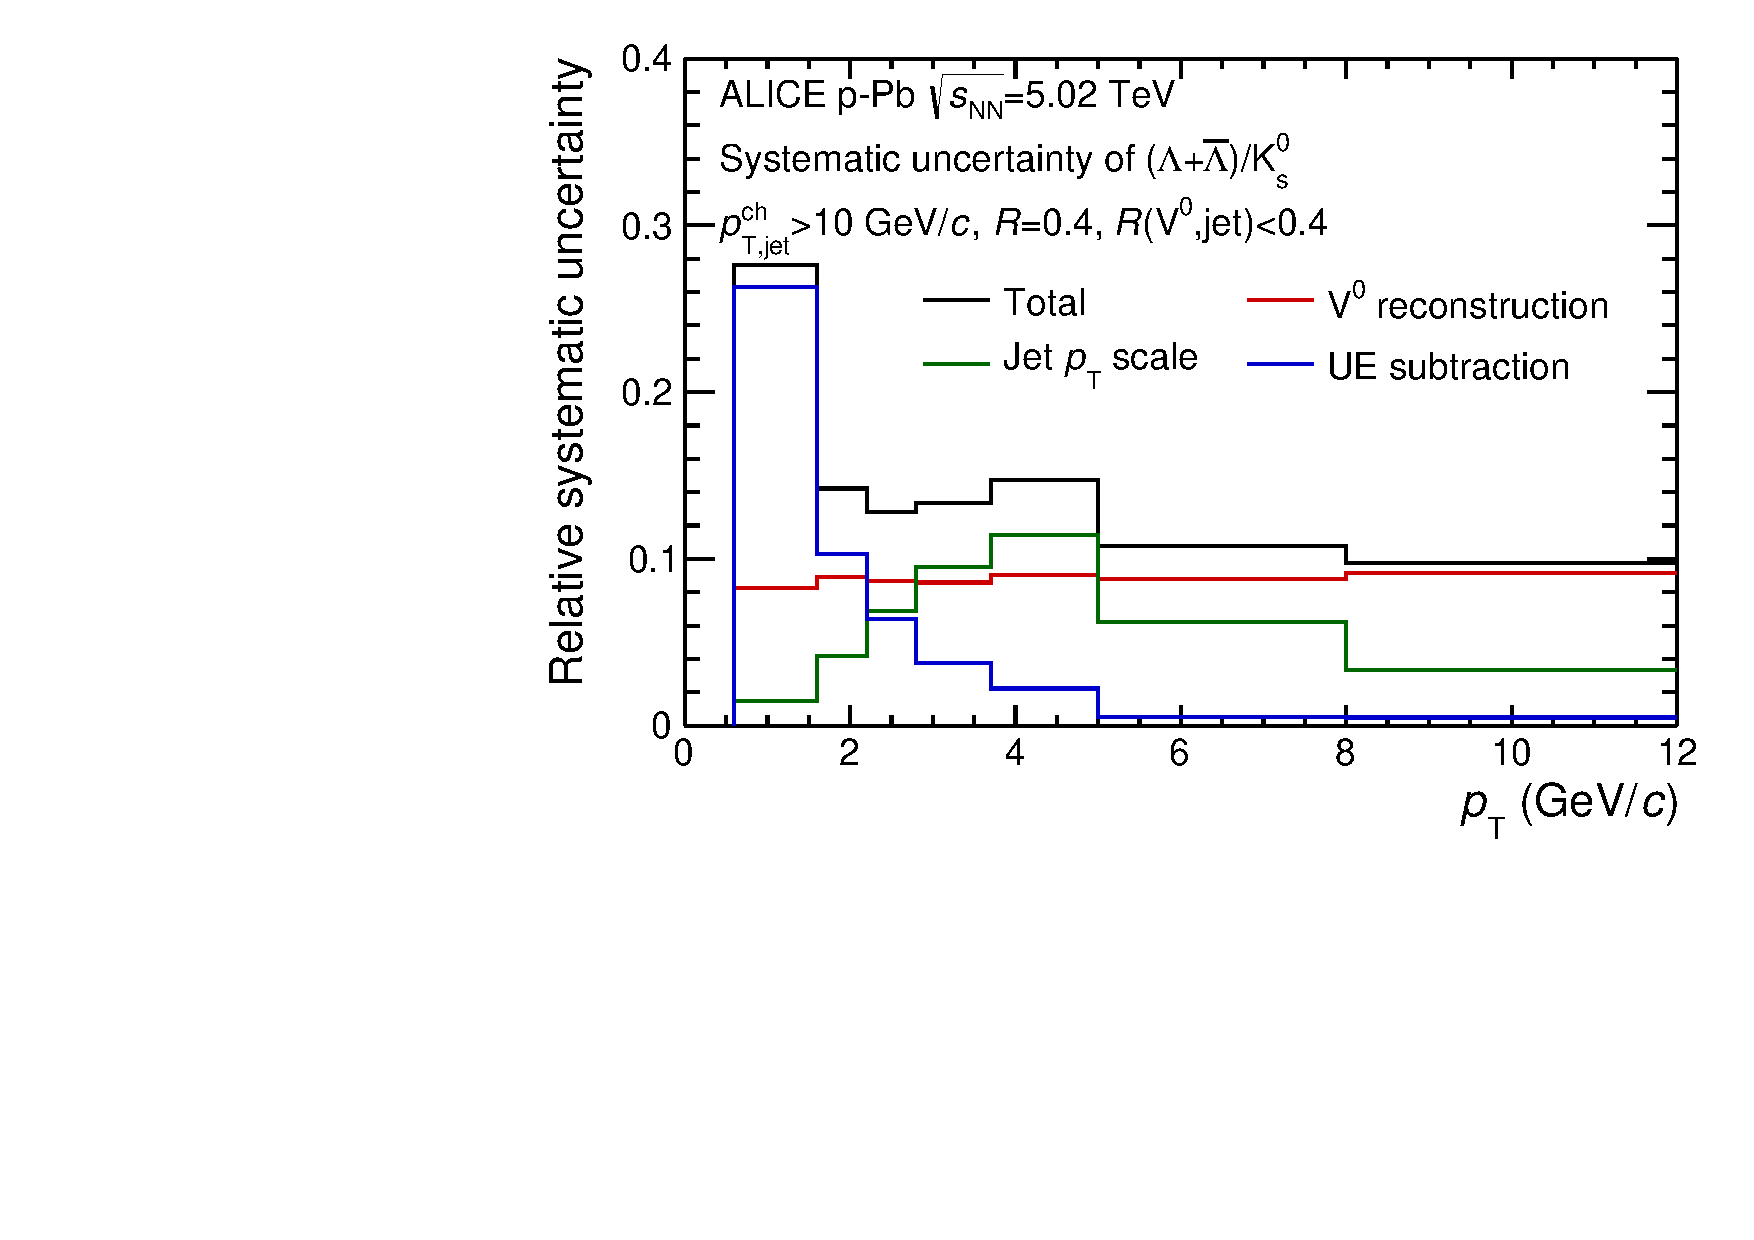
\includegraphics[width=0.32\textwidth]{cFig4a_pPb}
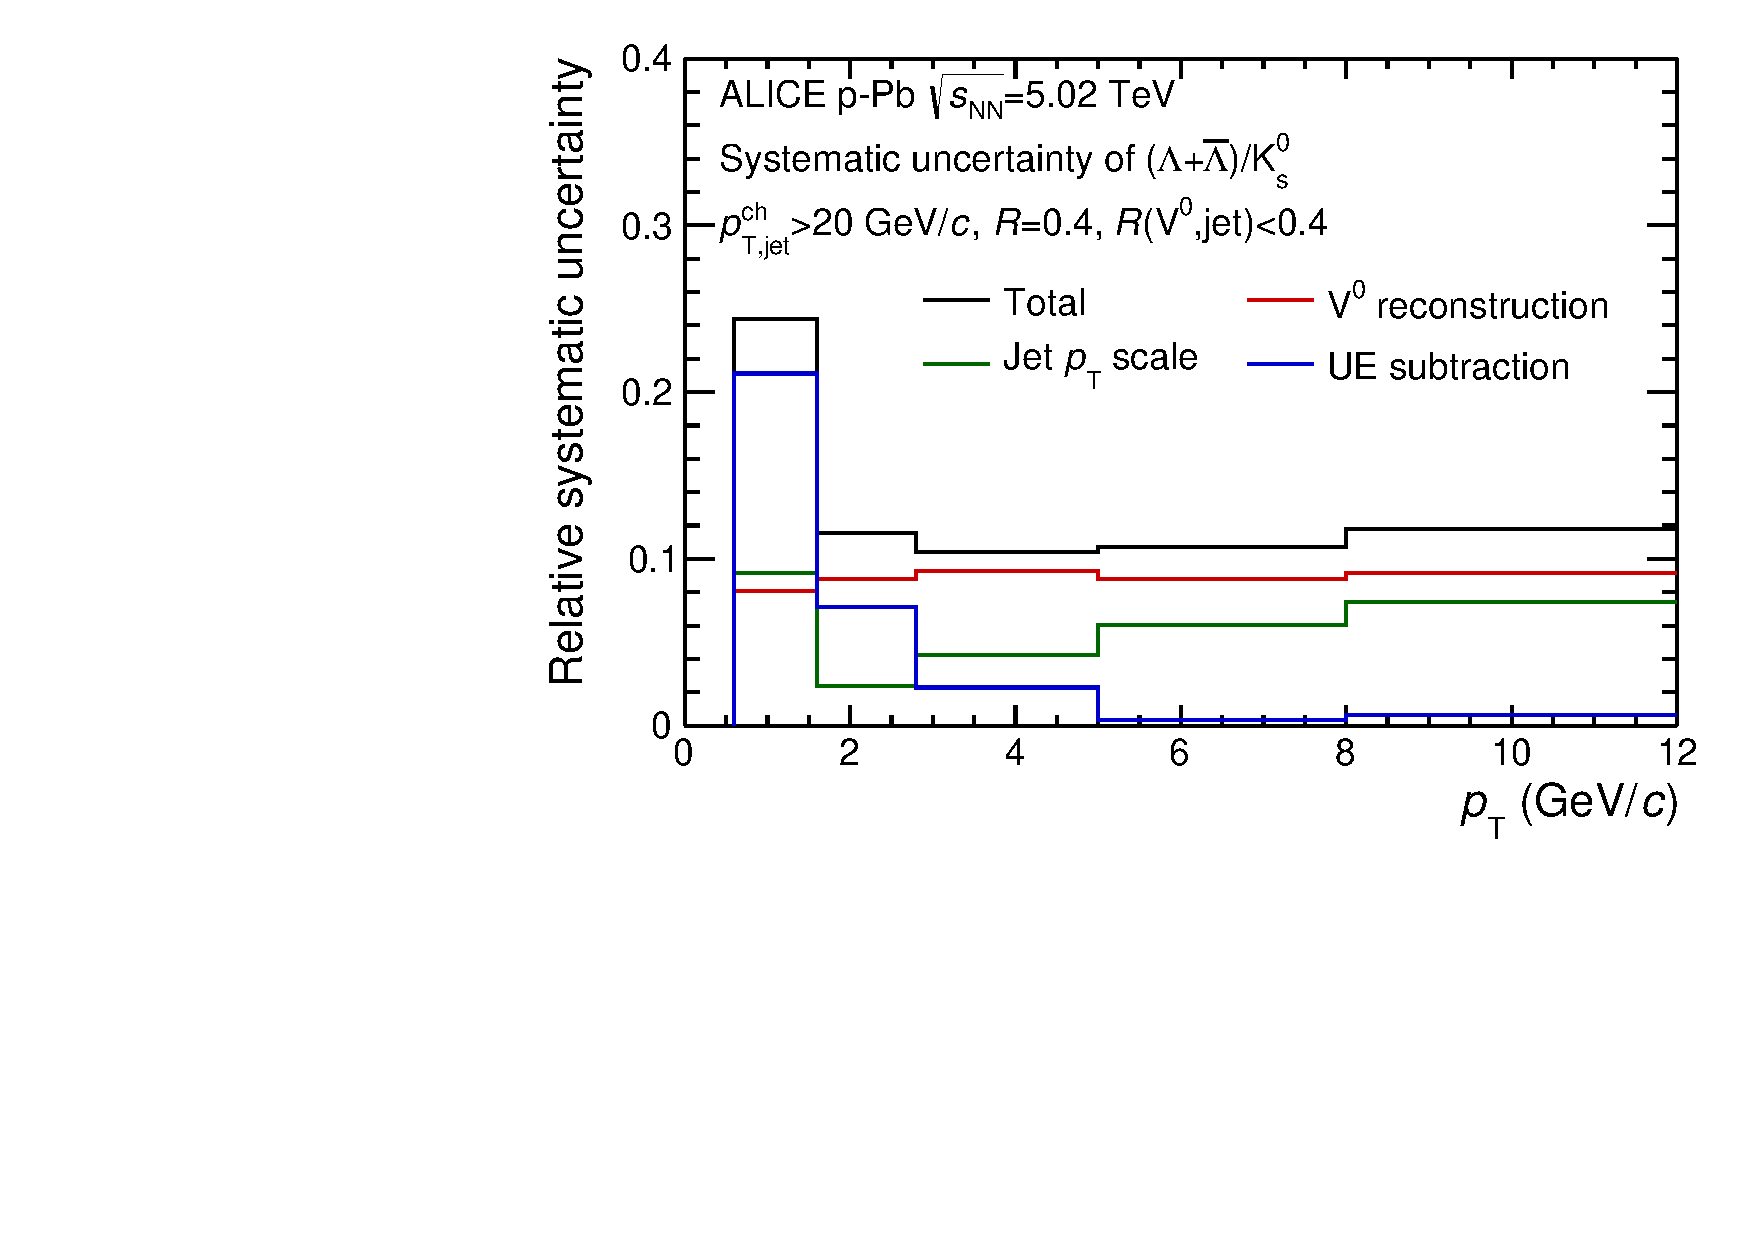
\includegraphics[width=0.32\textwidth]{cFig4b_pPb}
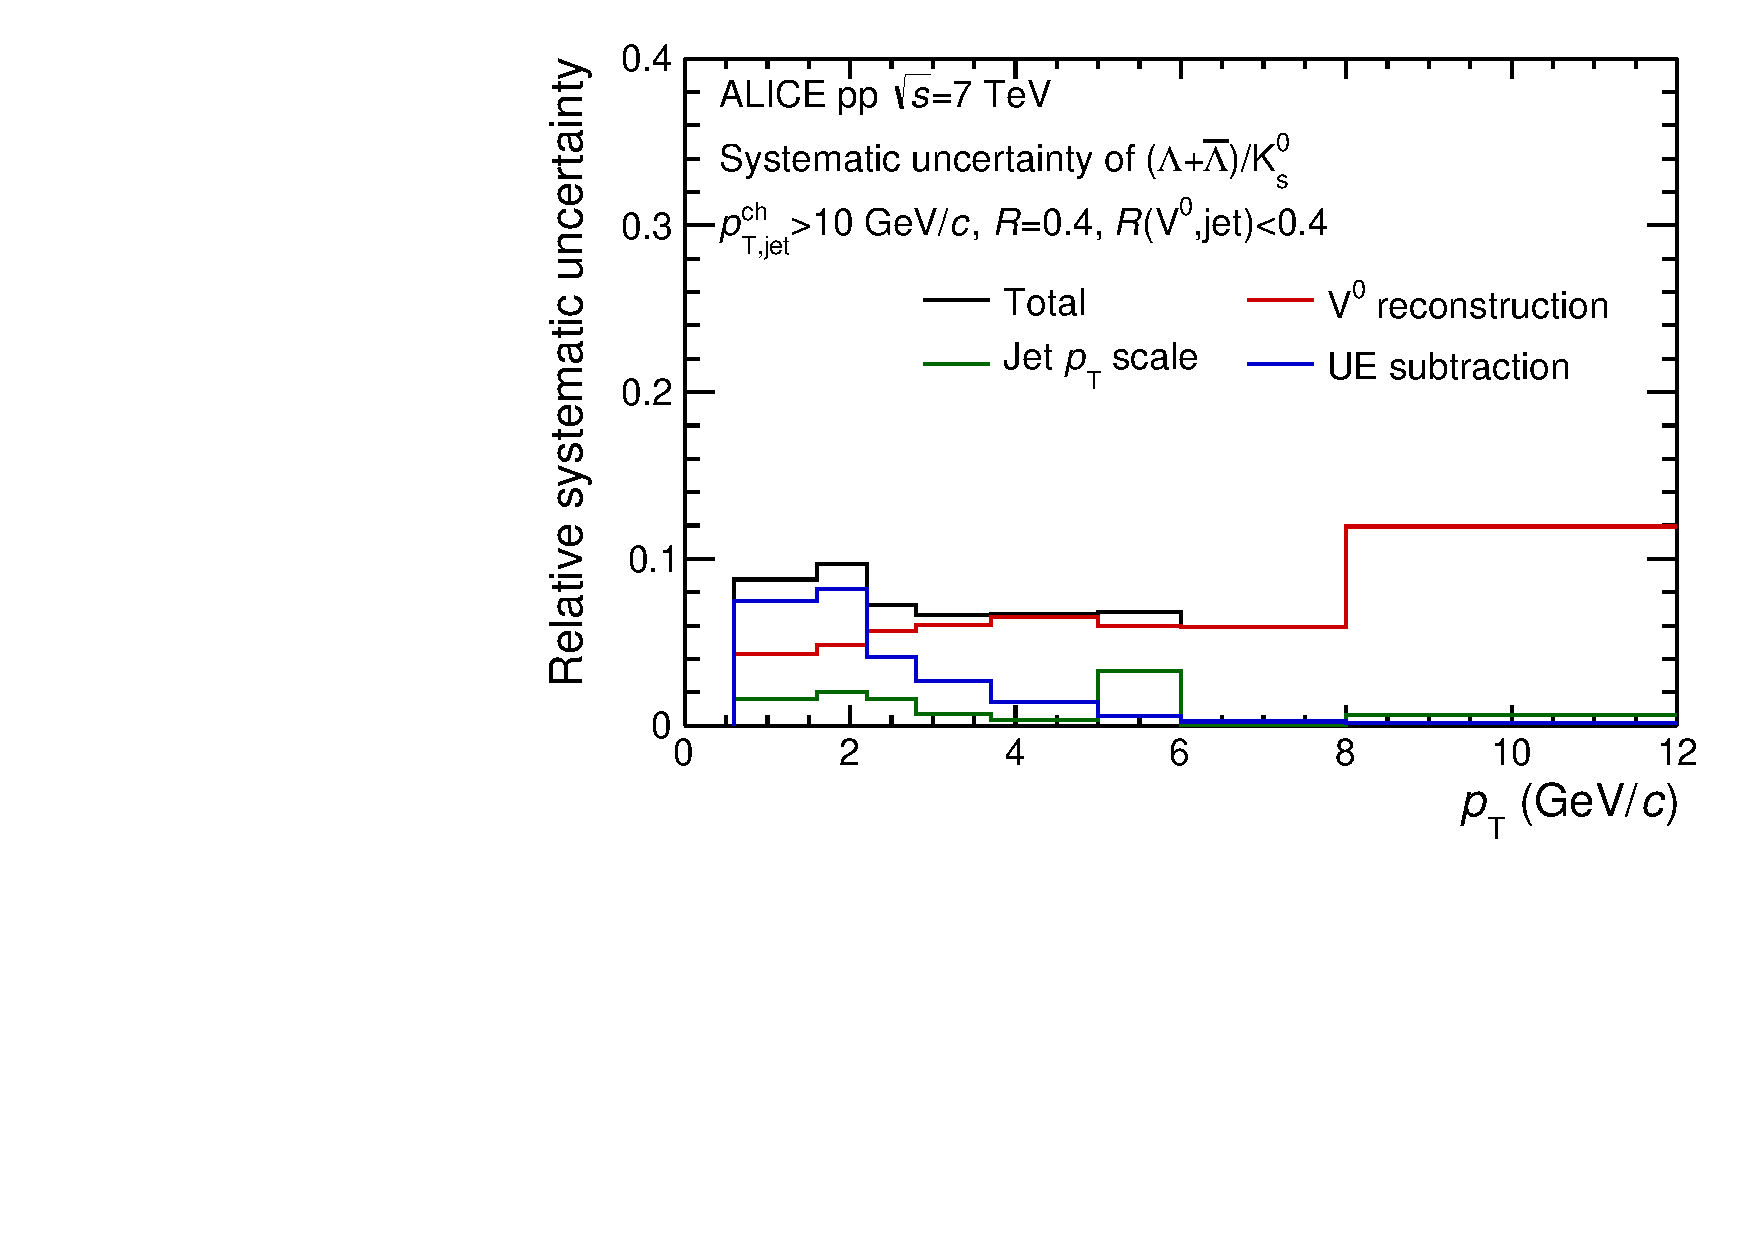
\includegraphics[width=0.32\textwidth]{cFig5_pp}
\caption{Relative systematic uncertainties on the ratio of the spectrum of \lda\ and \ks\ within $R=0.4$ anti-\kt\ jets for $\ptch>10~\gevc$ (left) and $\ptch>20~\gevc$ (middle) as a function of particle \pt\ in \pPb\ collisions at \sqrts{5.02}, and for jets for $\ptch>10~\gevc$ in pp collisions at \sqrts{7} (right).
Three contributions to the total uncertainty are shown: uncertainty on \vzero\ reconstruction, uncertainty on the underlying event subtraction, and uncertainty on the jet momentum scale and momentum resolution.}
	\label{fig:systUncertRatio}
\end{figure}

\subsection{Systematic uncertainties}
\label{sec:uncertainties}

The main sources systematic uncertainty in the \Vzero\ particle reconstruction are the level of knowledge of the detector material (resulting in a 4\% uncertainty), the track selection (up to 4\%), the feed-down correction for the \lda\ (5\% for $\pt<3.7~\gevc$ and 7\% for $\pt>3.7~\gevc$), the proper lifetime selection criteria (up to 3\%) and the topological selections that contribute up to 1.5\% depending on transverse momentum and particle species.

The $\pT$-dependent uncertainties on the extracted yields of \Vzero\ particles are shown in Fig.~\ref{fig:systUncert} for \ks\ mesons and \lda\ and \alda\ baryons in \pPb\ (upper pads) and pp (lower pads) collisions.
To calculate the total uncertainty on the yields the individual uncertainties on track selection, material budget, feed-down corrections and the listed \Vzero\ selections are added in quadrature.

{\bf Particle identification (PID).} Uncertainty due to the particle identification cuts was estimated by varying the cuts on the $\dedx$ in the TPC from a default $5 \sigma$ to 4, 6 and 7 standard deviations from the nominal $\dedx$ for pions and protons.

{\bf Track selection.} Uncertainty on the \Vzero\ yields originating from the track selection was estimated by repeating the analysis with the increased number of required TPC space points per track by about 7\% and 15\% from the nominal requirement of 70 points.

{\bf Topological selection.} The uncertainty associated to topological cuts on the \Vzero\ candidates (the two dimensional decay radius, daughter track DCA to primary vertex, DCA of \Vzero\ daughters, and cosine of the pointing angle) was obtained by varying the parameters of the selections for each of the \Vzero\ species separately as described in detail in \cite{Abelev:2013haa}.

{\bf Proper lifetime selection.} The uncertainty due to the cuts on the proper lifetime of the \Vzero\ candidates defined as the product of mass $m$, decay length $L$ and the inverse of particle's momentum $p$ ($mLc/p<20~{\rm cm}$ for \ks\ and $mLc/p<30~{\rm cm}$ for \lda\ and \alda) was obtained by redoing the analysis with different cuts (12 and 40 ${\rm cm}$ for \ks\ and 20 and 40 ${\rm cm}$ for \lda\ and \alda).

{\bf Competing \Vzero\ selection.} To obtain the uncertainty related to the cut on the competing \Vzero\ particles defined as the absolute mass difference between \Vzero\ candidate and the rest mass of the competing weakly decaying hadron ($m>5~\mevcc$ for \ks\ and $m>10~\mevcc$ for \lda) the analysis was repeated with 3 and 6 \mevcc\ for \ks\ and with no rejection for \lda\ baryons.
%%%%%%%%%%%%%%%%%%%%%%%%%%%%%%%%%%%%%%%%%%%%%%%%%%%%%%%%%%%%%%%%%%%%%

%\begin{figure}[!ht]
%\centering
%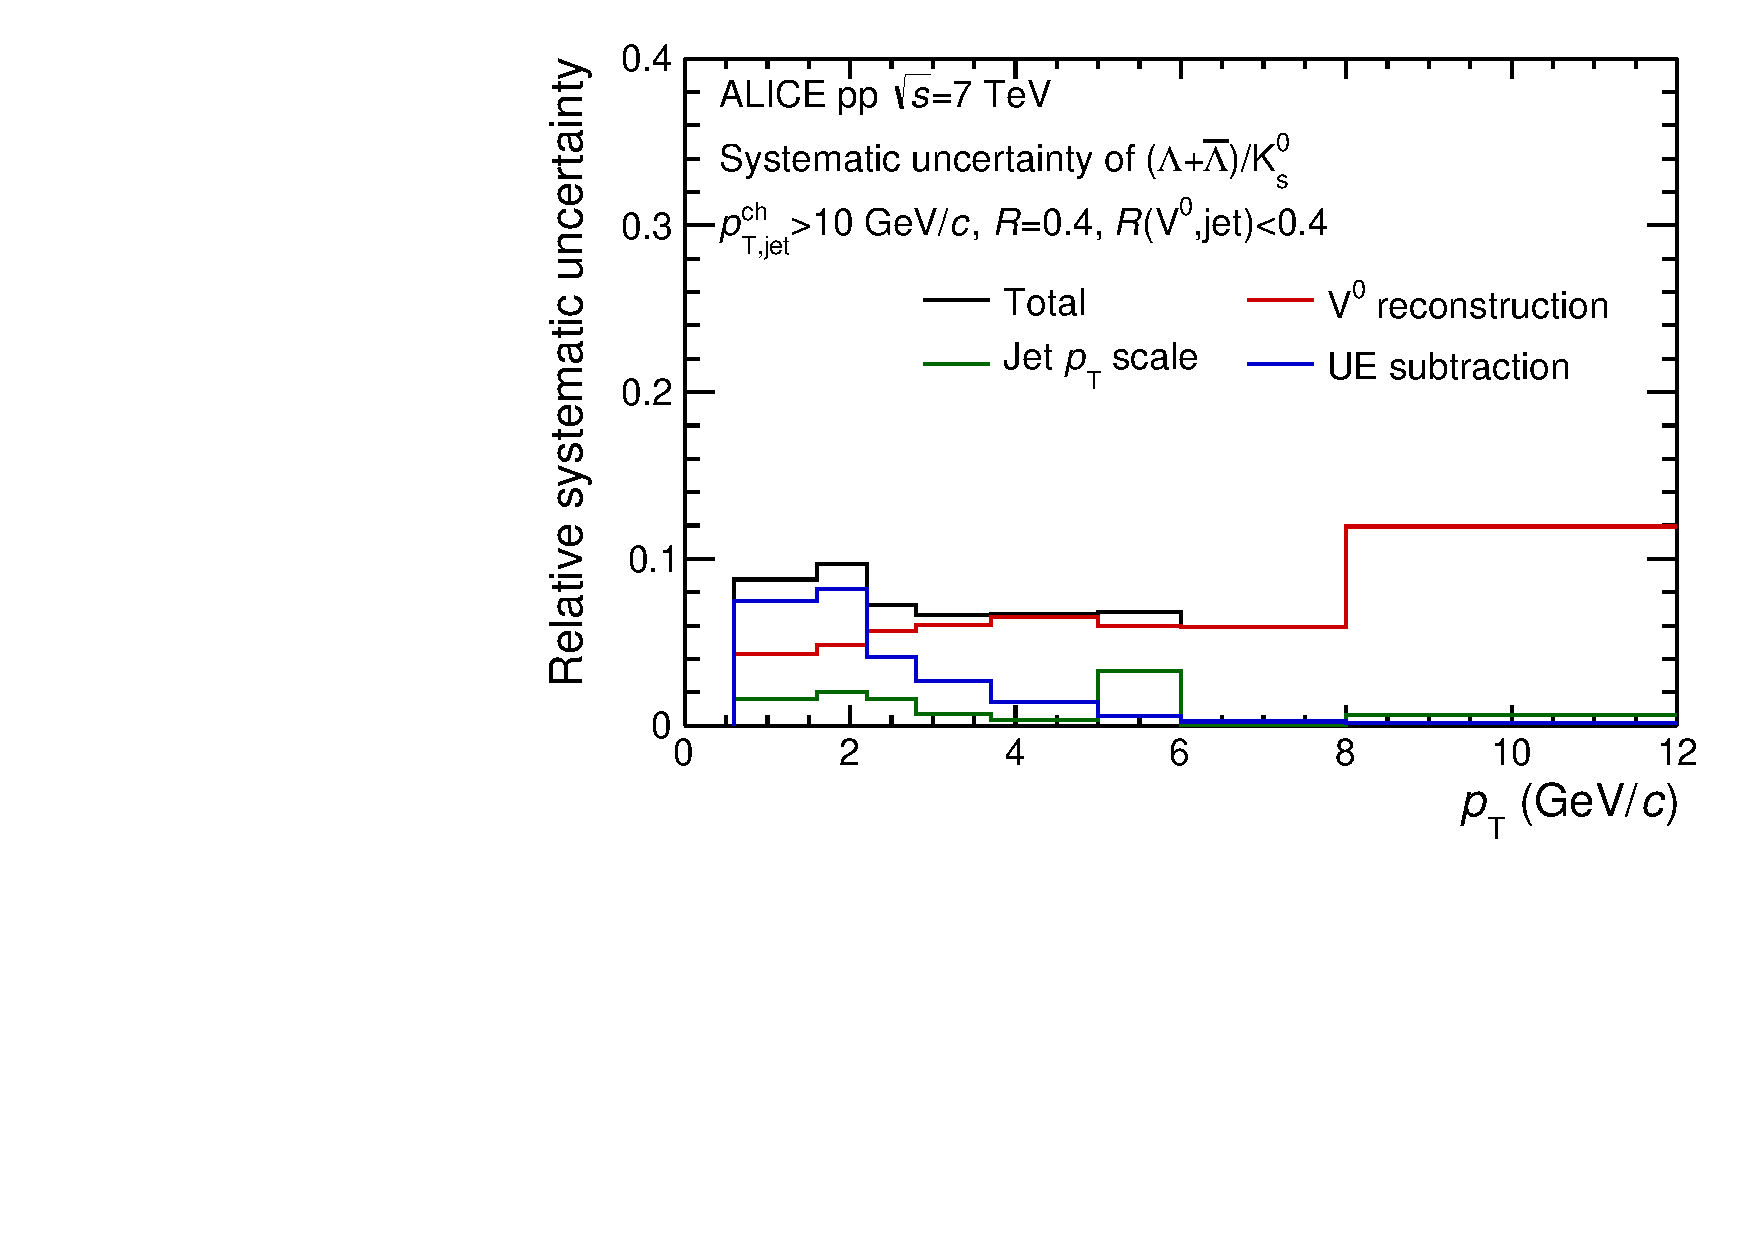
\includegraphics[width=0.8\textwidth]{cFig5_pp}
%\caption{Relative systematic uncertainty on the ratio of \lda\ and \ks\ spectrum within $R=0.4$ anti-\kt\ jets for $\ptch>10~\gevc$ as a function of particle \pt\ in \pp\ collisions at \sqrts{7}. Three contributions to the total uncertainty are shown: uncertainty on \vzero\ reconstruction, uncertainty on the underlying event subtraction and uncertainty on the jet momentum scale and momentum resolution.}
%\label{fig:systUncertRatio_pp}
%\end{figure}


{\bf Uncertainty on the yields in the underlying event.} Two main sources of uncertainties originating from the mis-association of \Vzero\ particles with the UE were considered: i) the \Vzero\ particle was found outside the selected jet and classified as a UE particle; however, it may have originated from a physical jet outside the fiducial acceptance for jets considered in the analysis and/or from a {\it true} low-\pt\ jet, below the considered thresholds; and ii) the \Vzero\ particle originates from a true high-\pt\ jet; however, due to the finite detector efficiency the jet has not been reconstructed above the considered \pt\ threshold.

The uncertainty on the UE \Vzero\ density has been estimated using the two variations of between UE estimators: the {\it outside cone} (OC) and the {\it non-jet events} (NJ).
The OC and the NJ estimators encapsulate the maximum deviation in the yield of UE particles. The standard deviation of the difference of the reconstructed \Vzero\ yields in OC and NJ has been included as the additional systematic uncertainties on the density of particles within the jets (JC).
In \pPb\ collisions the uncertainty is largest for low-momenta particles ($< 2~\gevc$) reaching up to 30\% but drops rapidly with \pt\ to negligible values for $\pt > 6~\gevc$.
While for \pp\ collisions the trend of the uncertainty is similar to the trend seen in \pPb\ but the magnitude is smaller, reaching values up to 8\%.
%%%%%%%%%%%%%%%%%%%%%%%%%%%%%%%%%%%%%%%%%%%%%%%%%%%%%%%%%%%%%%%%%%%%%

{\bf Uncertainty on yields in jets.} The systematic uncertainty originating from the selection of the jet \pt\ was estimated by repeating the analysis with jet \pt\ varied around the chosen thresholds of 10 and 20~\gevc\ by 2~\gevc.
This variation accounts for jet resolution due to detector effects and the fluctuations of the event background density as reported in \cite{Adam:2015hoa}.
For jets with $\ptch>10~\gevc$ at low momenta ($\ptvzero<2~\gevc$) it reaches up to 10\% while it is about 20\% for jets of $\ptch>20~\gevc$.
The uncertainty remains almost constant of about 3\% for $\ptvzero > 2~\gevc$ for jets $\ptch>10~\gevc$ and about 5\% for jets $\ptch>20~\gevc$.

{\bf Uncertainty on the \lda/\ks\ ratio.} The uncertainties on \Vzero\ yields, material budget and feeddown correction are propagated to the ratio quadratically.
The uncertainties related to~ the jet \pt\ and UE estimation are obtained by calculating the deviation of ratios between the default analysis and various selections.
Figure~\ref{fig:systUncertRatio} shows the relative systematic uncertainties on the $(\lda+\alda)/(2\ks)$\ ratio reconstructed within $R=0.4$ jets with $\ptch > 10~\gevc$ (left) and $\ptch > 20~\gevc$ (middle) as a function of particle \pt\ in \pPb\ collisions.
For the $\ptch > 20~\gevc$ the total uncertainty is about 16\% and is largely independent of particle \pt\ with the largest contribution of 14\% originating from the uncertainty on \Vzero\ reconstruction.
The relative systematic uncertainties on the $(\lda+\alda)/(2\ks)$\ ratio for \pp\ collisions are shown in the right plot in %Fig.~\ref{fig:systUncertRatio_pp}.
Fig.~\ref{fig:systUncertRatio}.
%%%%%%%%%%%%%%%%%%%%%%%%%%%%%%%%%%%%%%%%%%%%%%%%%%%%%%%%%%%%%%%%%%%%%

\begin{figure}[!t]
\centering
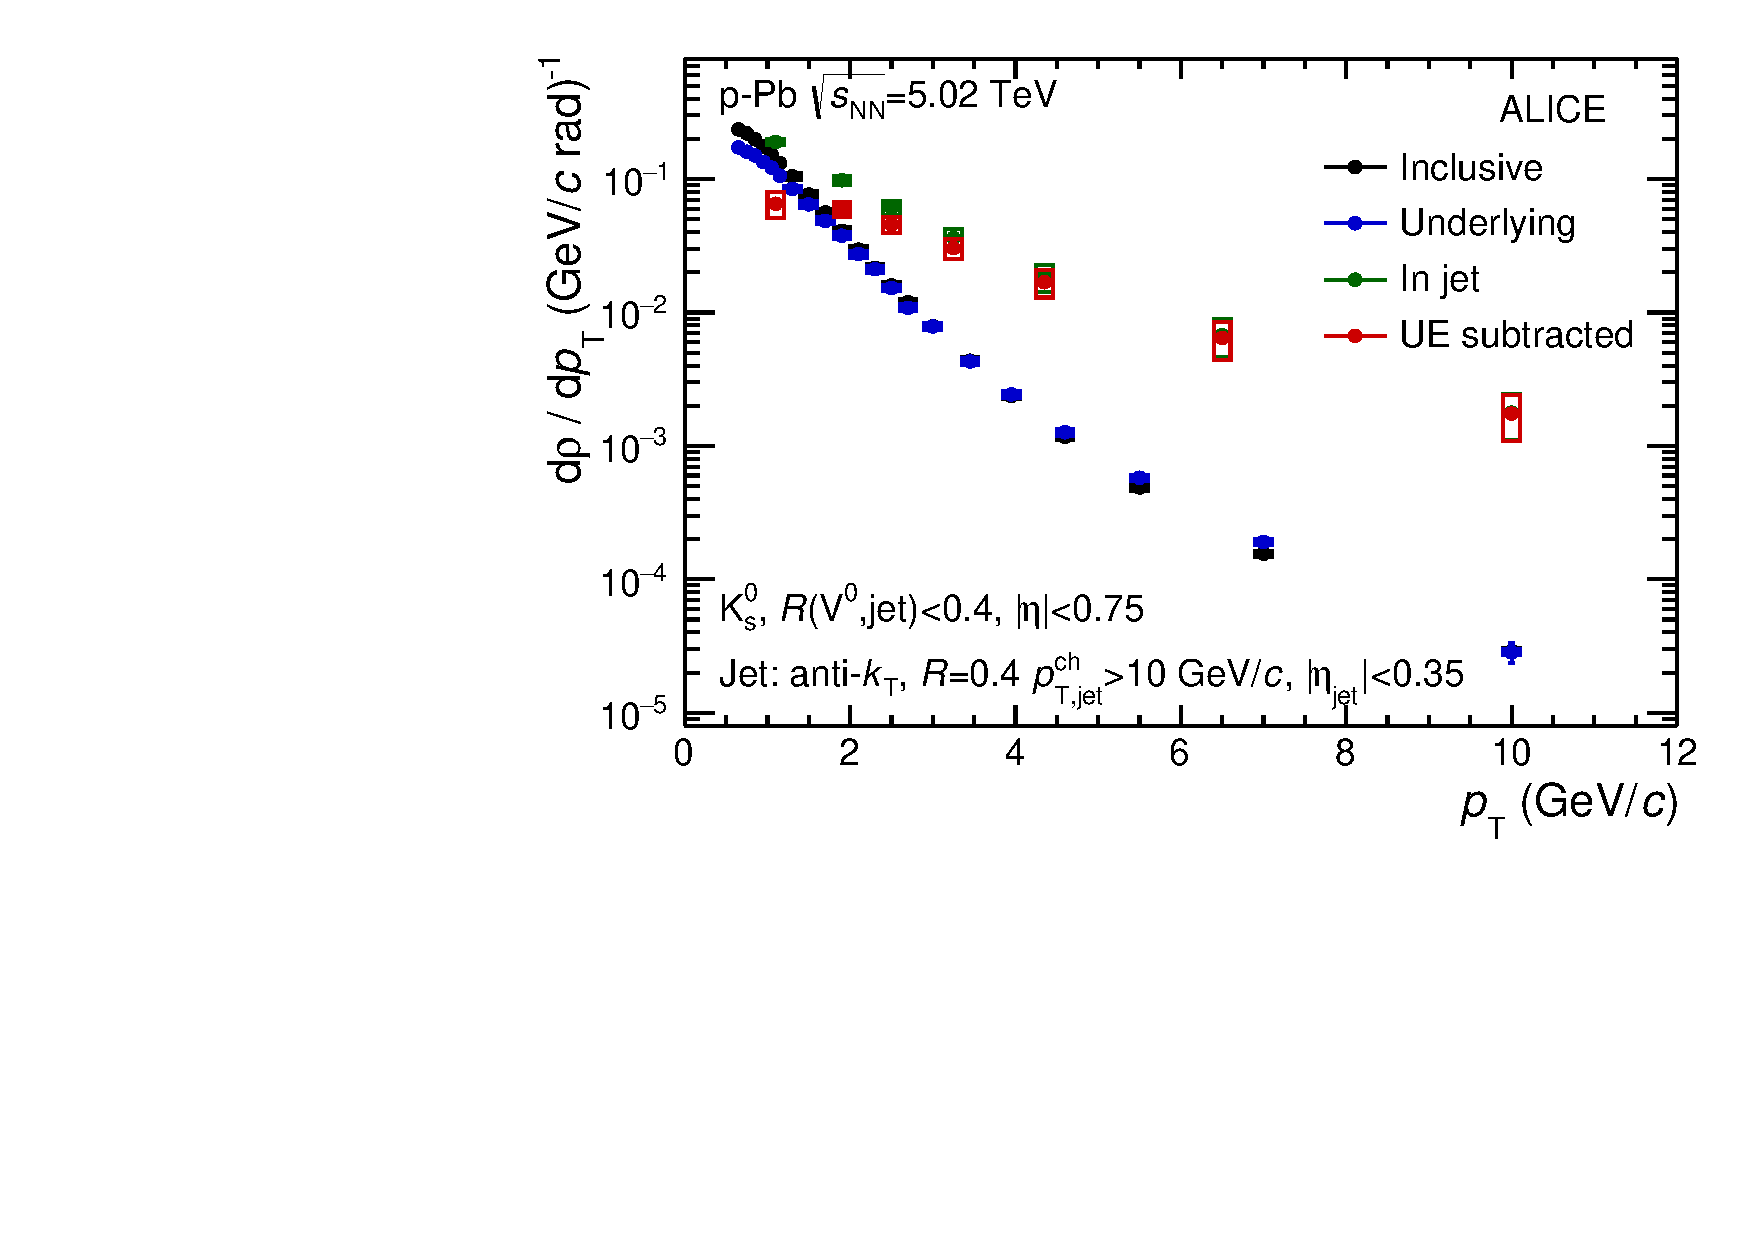
\includegraphics[width=0.49\textwidth]{cFig6a_pPb}
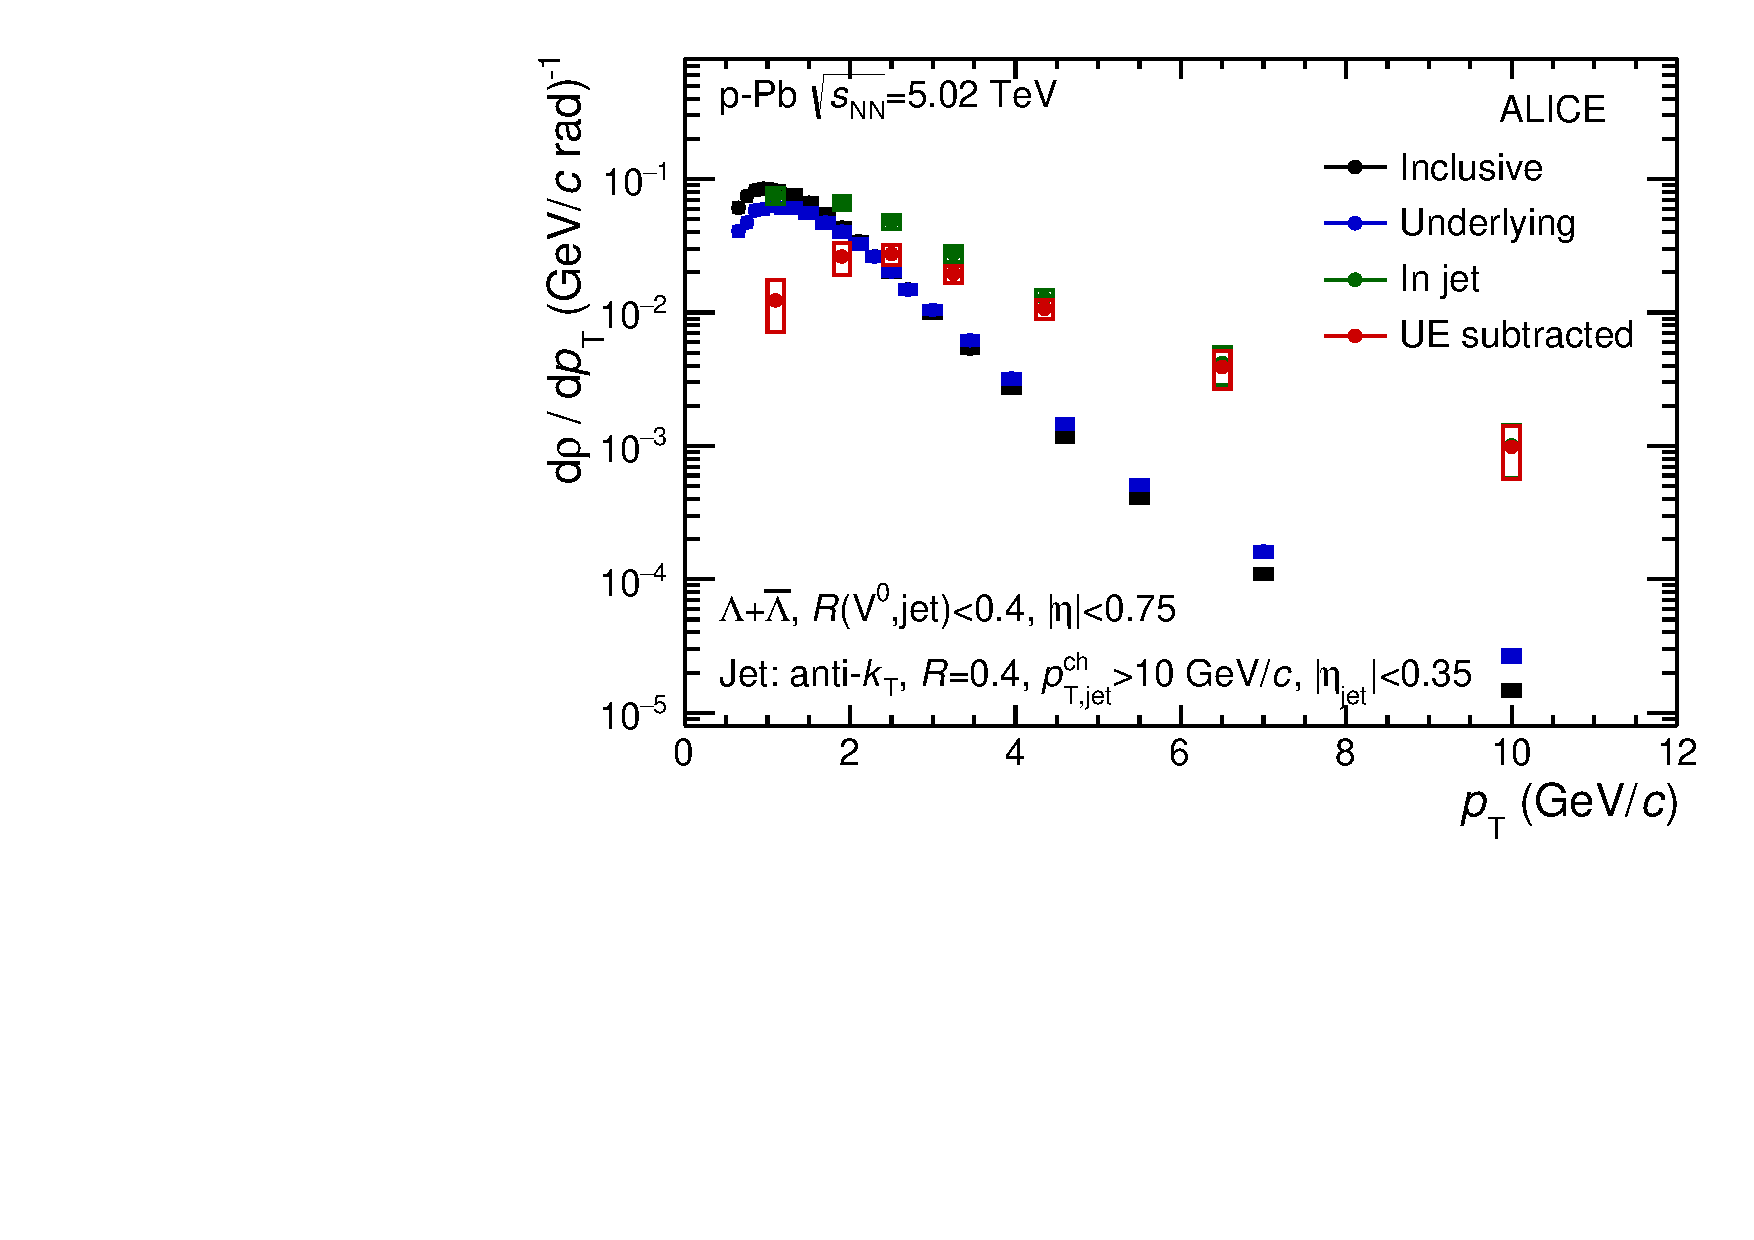
\includegraphics[width=0.49\textwidth]{cFig6b_pPb}
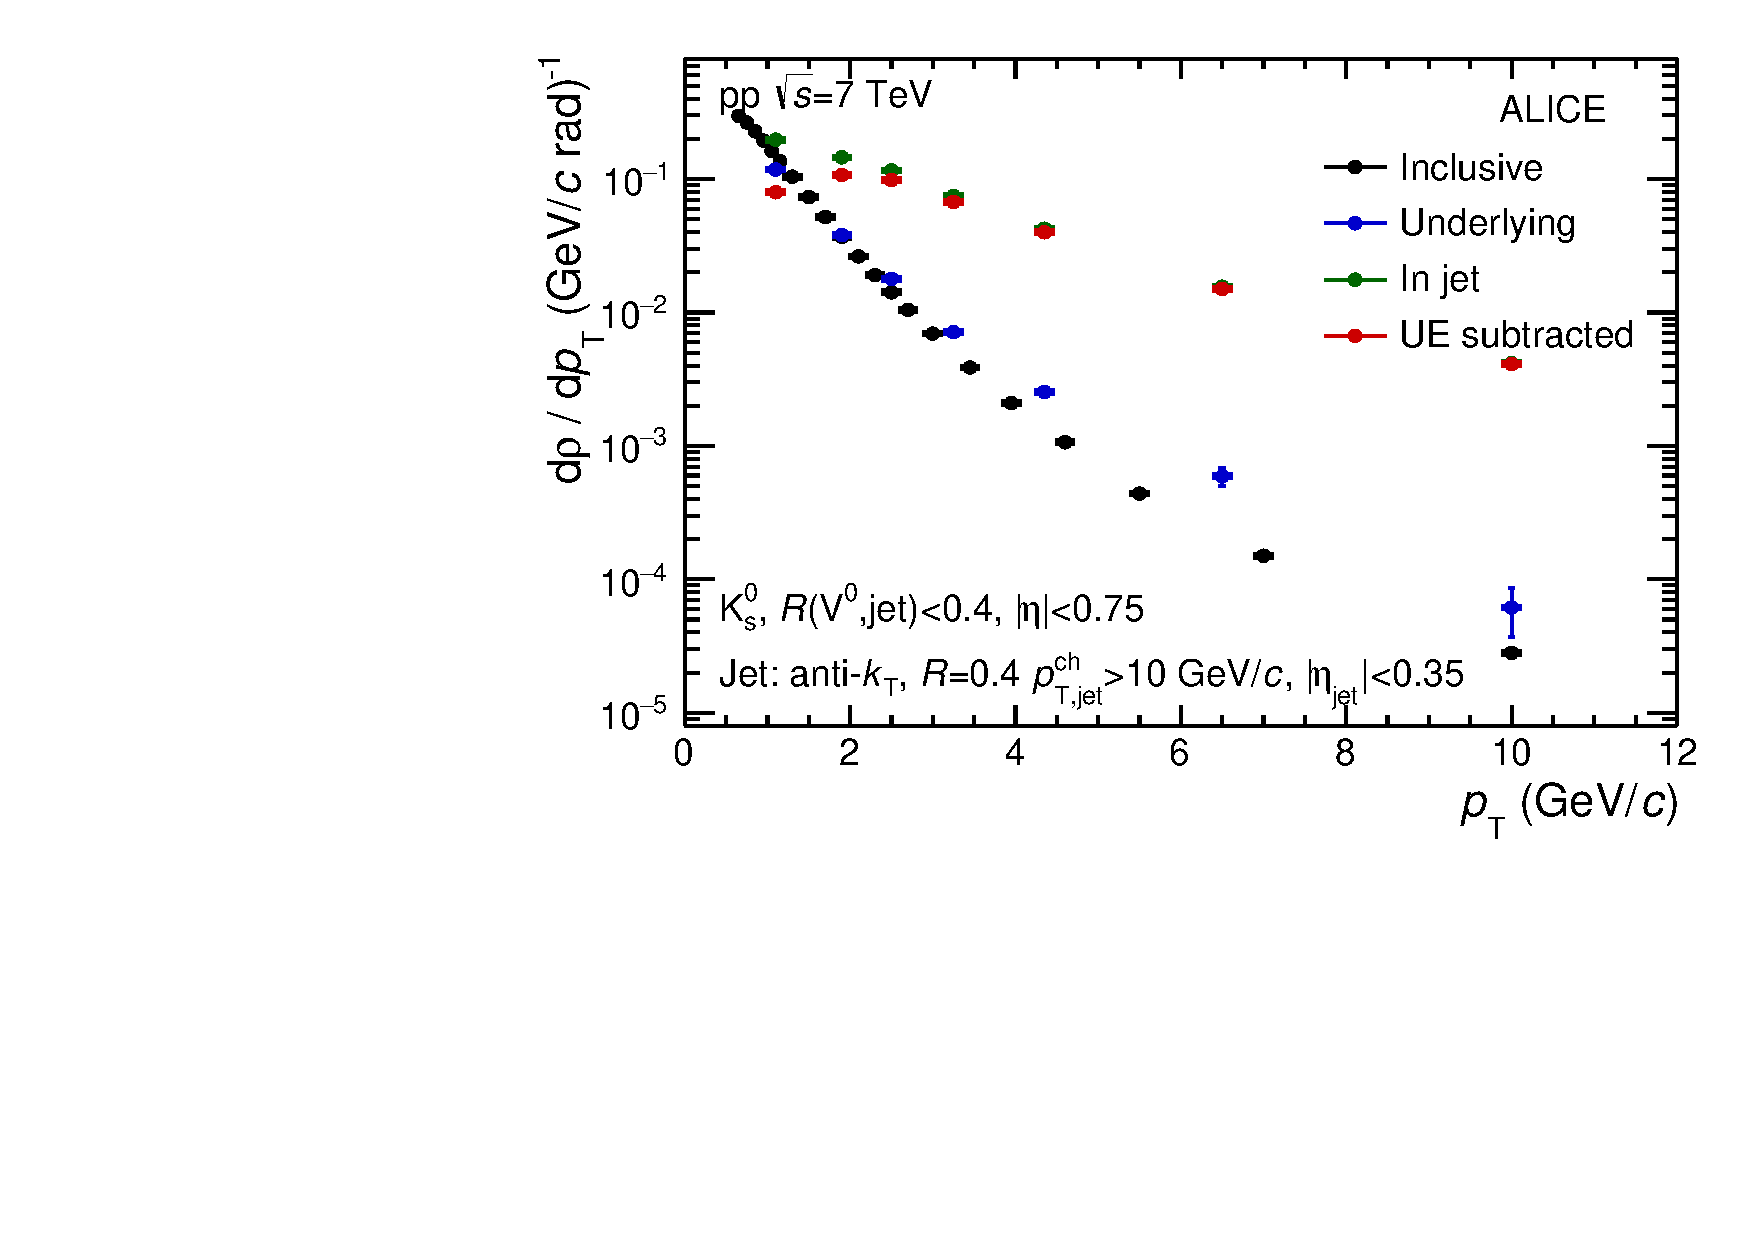
\includegraphics[width=0.49\textwidth]{cFig6c_pp}
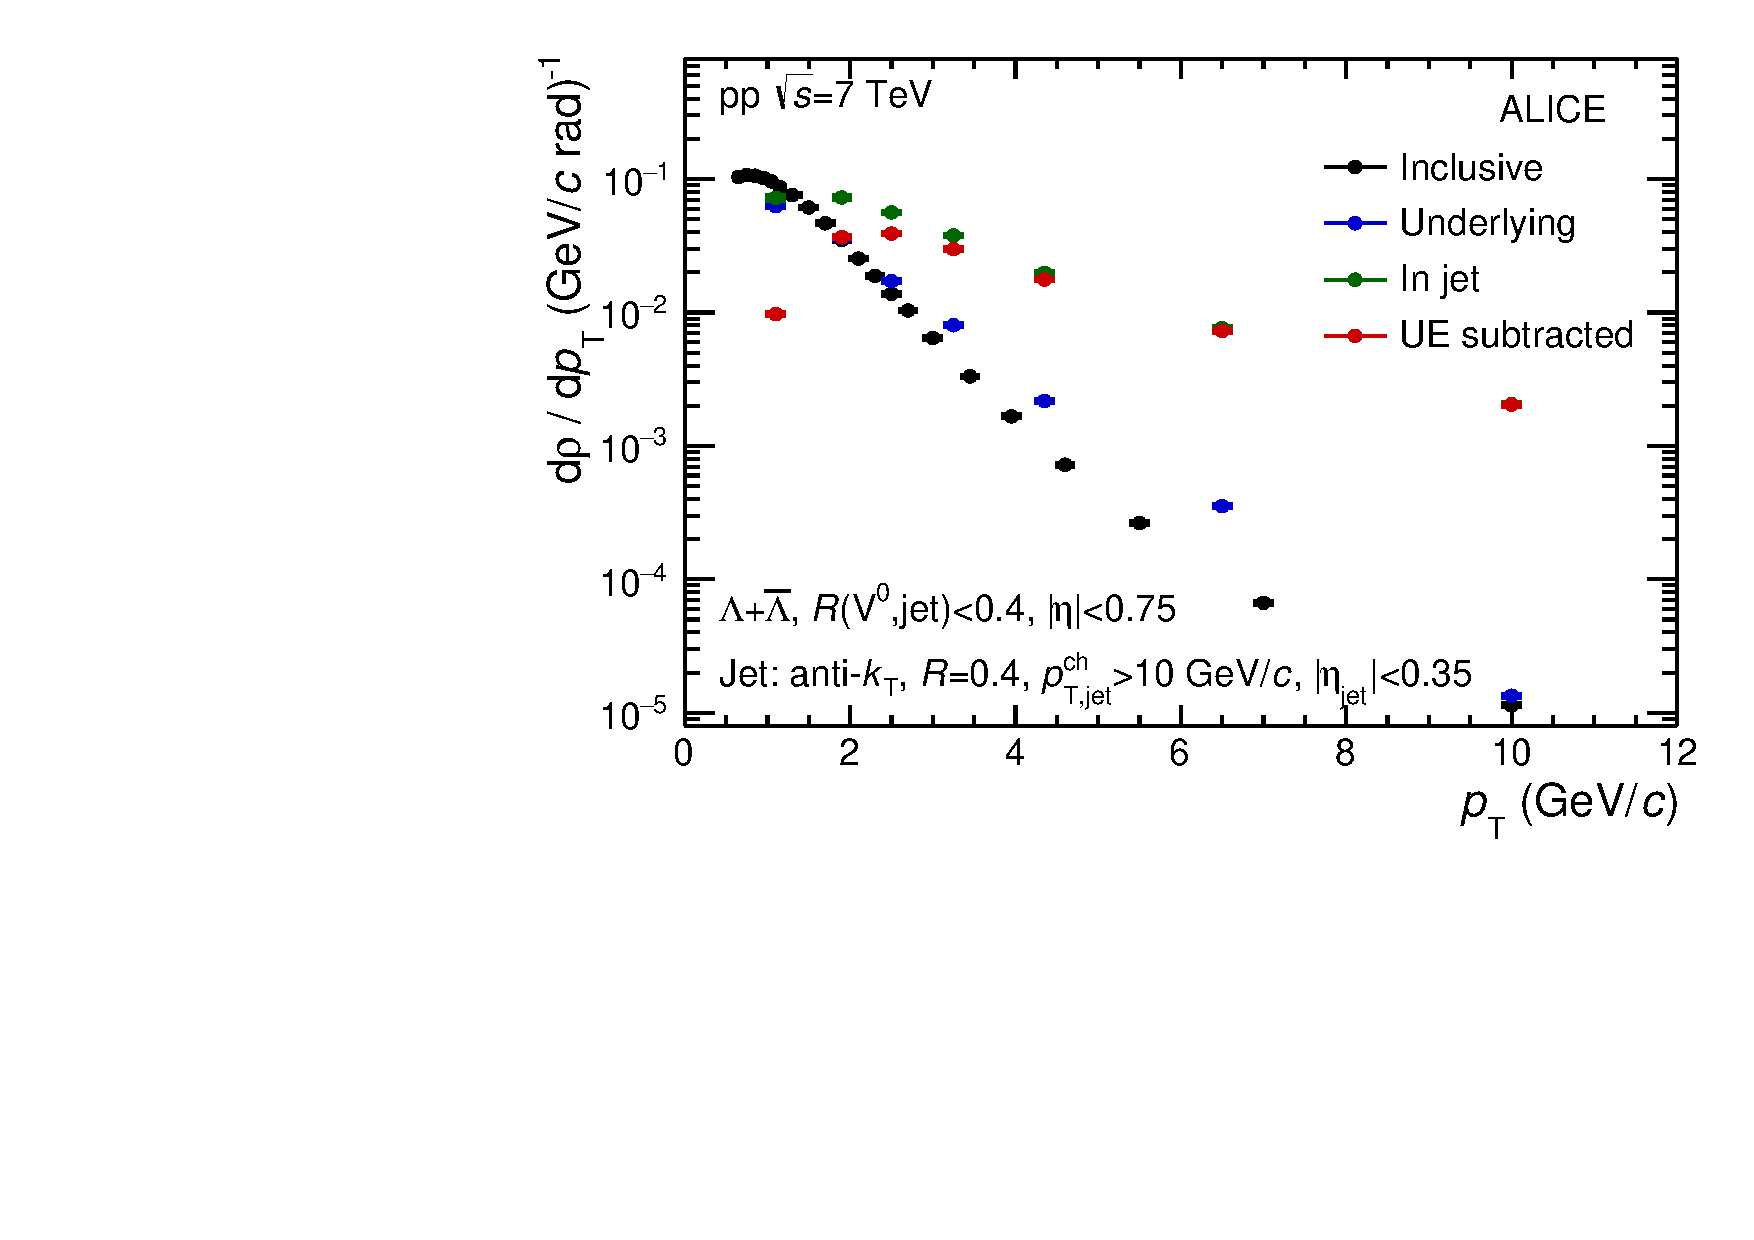
\includegraphics[width=0.49\textwidth]{cFig6d_pp}
\caption{$\pT$-differential density of particles \drhodpt\ (see Eq. \ref{eq:defv0rho}) in \pPb\ collisions at \sqrtsnn{5.02} (upper) and  in \pp\ collisions at \sqrts{7} (lower) for \ks\ (left), and the sum of \lda\ and \alda\ (right). The density is shown for three selections: inclusive particles from minimum bias events (black), particles within anti-\kt\ jets ($\ptch>10~\gevc$) with $R=0.4$ (green) and particles associated with the underlying event production estimated within perpendicular cone (PC) in events containing jets (blue).}
\label{fig:rhov0}
\end{figure}

\section{Results}
\label{sec:Results}

\subsection{\pt-dependent densities of \vzero\ particles}

The fully corrected densities of \ks\ and the sum of \lda\ and \alda\ particles associated to a hard scattering tagged by a jet are shown in Fig.~\ref{fig:rhov0} for \pPb\ and \pp\ collisions.
The per-jet density within the jet cone (JC) is compared to the density for inclusive particles (irrespective of their association to a hard scattering) and to the density of underlying event \vzero s estimated in the perpendicular cones (PC).
In the case of inclusive particles the distribution is normalized to the product of the total number of events and the acceptance of the \vzero\ particles in a single event (full azimuth and $|\eta|<0.75$).
As expected, for both \ks\ and \lda\ particles the \pt\ dependence of the density within jets, as defined by eq.~(\ref{eq:defv0rho}), is considerably less steep than the high-\pt\ particles originate from jets.
The density in the PC selection is qualitatively similar to the inclusive distribution showing a strong, steeply falling \pt\ dependence.
Both the inclusive and the PC distributions show a rapid decrease with \pt, reaching values more than an order of magnitude lower than the JC density for particle \pt\ exceeding $4~\gevc$.
This is consistent with the expectation that the high-\pt\ particles originate from jet fragmentation.

\subsection{$(\lda+\alda)/(2\ks)$ ratios}

Ratios of \lda\ and \ks\ yields can be obtained by dividing the normalized density distributions.
In the following the sum of \lda\ and \alda\ densities is divided by twice the density of \ks.
As no significant difference was found for different jet resolution parameters $R$ the results are presented as the average of results obtained with $R$ of 0.2, 0.3, and 0.4.

\begin{figure}[!t]
\centering
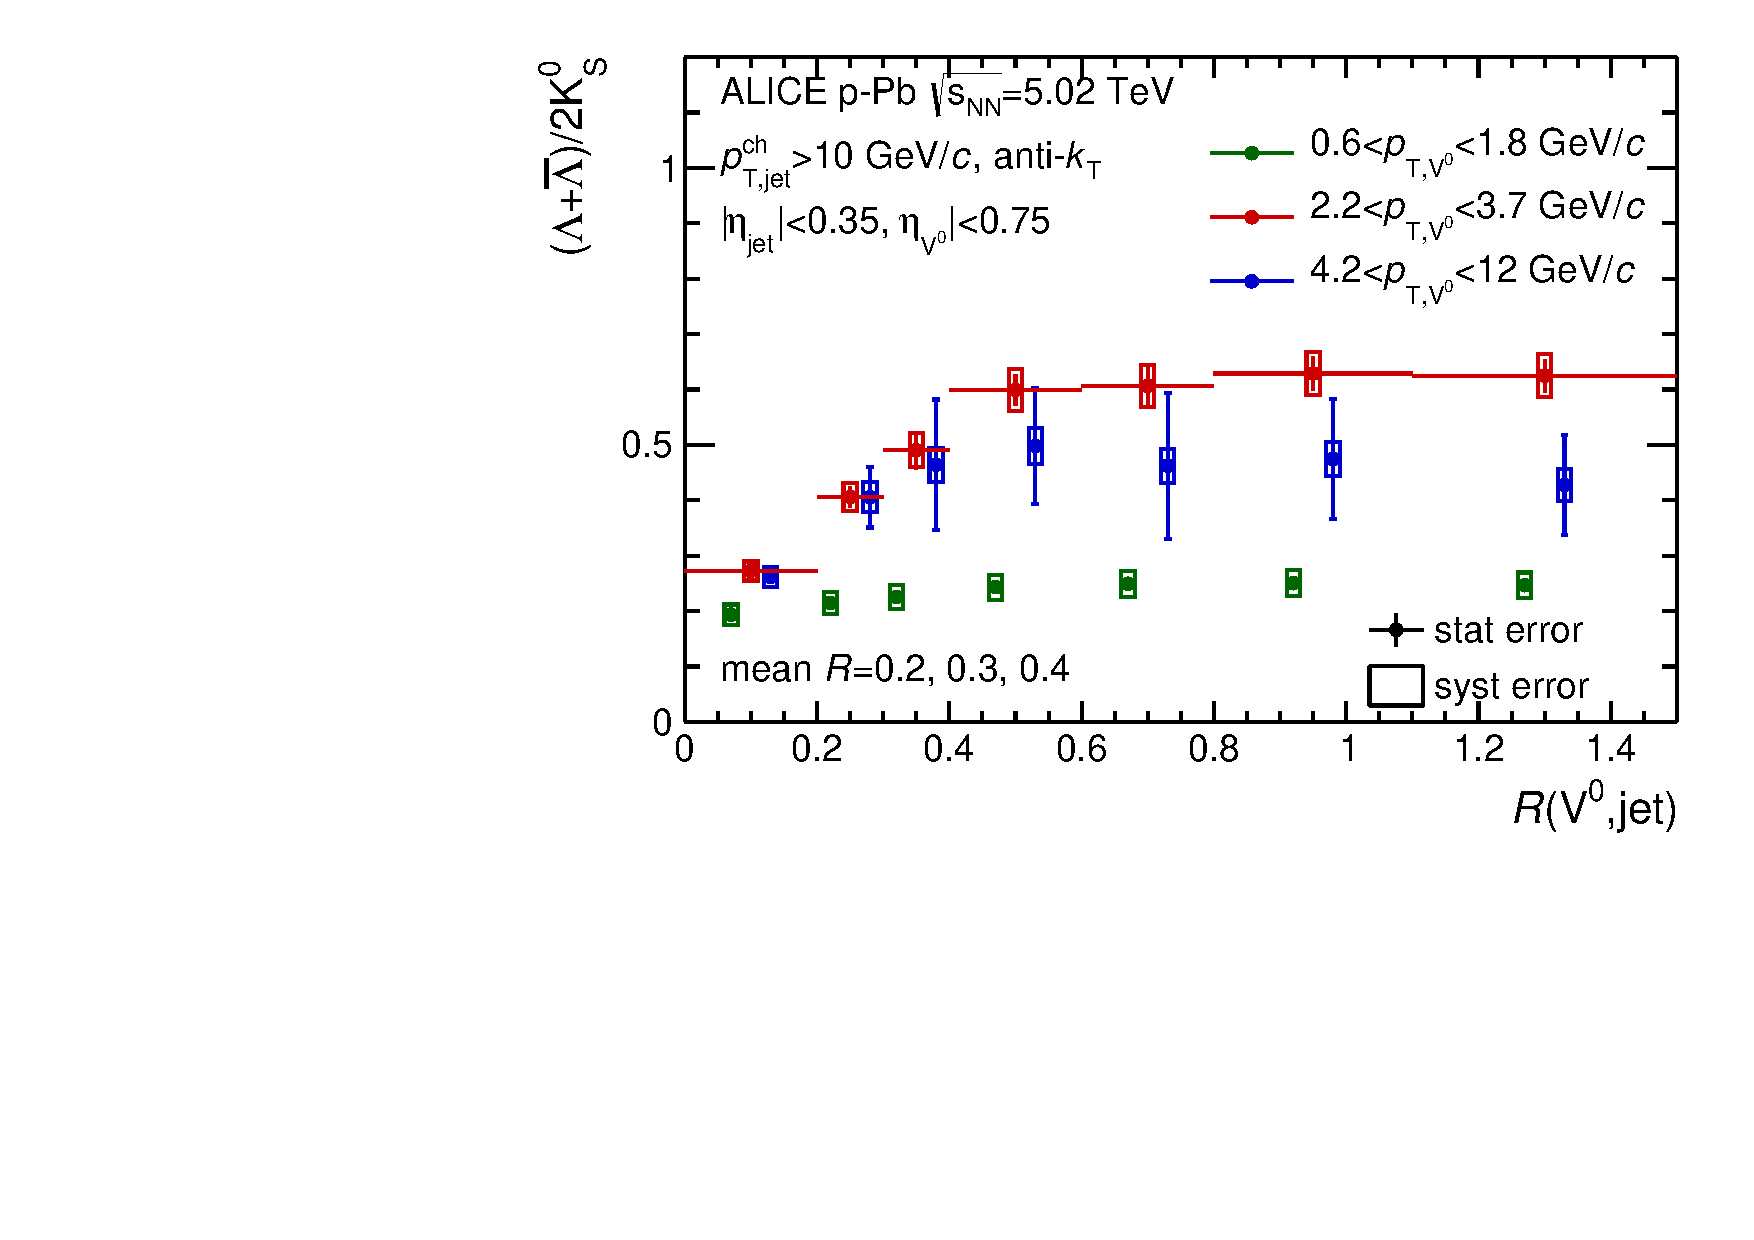
\includegraphics[width=0.80\textwidth]{cFig7}
\caption{\lda/\ks\ ratio in p--Pb collisions at \sqrtsnn{5.02} as a function of $R(\Vzero,{\rm jet})$ for three different \Vzero-particle \pt\ selections associated with charged jets with $\ptch>10~\gevc$.
The data points of ratios in $0.6<p_{{\rm T,V}^{0}}<1.8$~GeV/$c$ and in $4.2<p_{{\rm T,V}^{0}}<12$~GeV/$c$ are shifted to the left and right sides from the center, respectively, alone the $x$-axis.}
	\label{fig:LKR}
\end{figure}

Figure~\ref{fig:LKR} shows the ratio for the raw JC selection (JC yield without the UE background subtraction) as a function of the distance from the jet axis \rvzerojet\ in \pPb\ collisions.
The ratio is shown for three momentum bins: the low-\pt\ ($0.6 <\pt <1.8~\gevc$), intermediate \pt\ ($2.2 < \pt < 3.7~\gevc$), and the high-\pt\ ($4.2 < \pt < 12~\gevc$).
The ratio as a function of \rvzerojet\ at low-\pt\ remains, dominated by the UE contribution, approximately constant at about $0.2$ independent of the distance to the jet axis and that is the case even at large distances of $\rvzerojet > 1.2$.
This value is consistent with the inclusive measurements in \pPb\ collisions, but also in \pp\ and peripheral \PbPb\ collisions where effects related to the collective expansion of the system are either not present or small \cite{Abelev:2014uua}.

Conversely the intermediate-\pt\ selection shows an increase of the ratio from about $0.3$ when evaluated close to the jet axis to values of about $0.6$ at \rvzerojet\ distances of about $0.5$.
For distances $\rvzerojet > 0.5$ the ratio remains constant.
The ratio of $0.6$ is consistent with the inclusive measurement in \pPb\ collisions \cite{Abelev:2013haa} and this \pt\ region is where the enhanced \lda/\ks\ ratio in the inclusive measurements was found to be the largest.
We stress that for the results shown in Fig.~\ref{fig:LKR} the UE backgrounds were not subtracted.
Therefore the evolution of the ratio as a function of the distance from the jet axis demonstrates how the two sources UE and jet compete.
The lack of enhancement %(values consistent with \pp\ collisions)
close to the jet axis indicates that the enhanced \lda/\ks\ ratio is not associated with the jets.

In each of the momentum bins the ratio is dominated by the lower edge of the selection window due to steeply falling particle \pt\ spectrum.
This is especially the case for the high-\pt\ selection where the dominating component originates from \pt\ of about $4.5~\gevc$ and the \rvzerojet\ dependence at high-\pt\ is similar to intermediate \pt. The ratio at high-\pt\ associated to jets is discussed below.

Figure~\ref{fig:L2Kratio_pp_pPb} shows the ratio of \lda\ to \ks\ as a function of particle \pt\ in both \pp\ and \pPb\ collisions for several selections.
In the case of \pPb\ collisions the ratio for the inclusive particles, the particles from the PC selection, and two JC selections for jet \pt\ of $10$ and $20~\gevc$ averaged over three resolution parameters $R$ (0.2, 0.3, 0.4) is shown.
Prior to forming the ratio, the UE density contribution obtained with the PC selection was subtracted from the JC yields for each particle species separately.
Additionally, the \pPb\ results are shown for the case where every \Vzero\ particle was required to be close to the jet axis with its distance $\rvzerojet < 0.2$.
The inclusive and the PC distributions show the enhancement at \pt\ of about $3~\gevc$.
The measurement for the inclusive case differs from that in \cite{Abelev:2013haa} as the region $\abs{\eta}<0.75$ is used here instead of $0 < y_{\rm cms} < 0.5$. The two measurements are otherwise consistent with each other.
The PC distribution above $2~\gevc$ reaches systematically higher values than the inclusive.
The ratio within jets is consistently lower than the inclusive case and approximately independent of \pt\ beyond $2~\gevc$.
In particular, for particles associated to the jet it does not show a maximum at intermediate \pt.
Clearly the enhancement of the ratio seen in the inclusive measurement is not present within the jets.
This conclusion holds not only for jets with $\pT>10$~\gevc\ but also for higher \pt\ ($>20~\gevc$) jets.

The results for \pp\ collisions shown in Fig.~\ref{fig:L2Kratio_pp_pPb} were obtained with jets reconstructed with $R=0.4$ and for the same value of the matching radius $\rvzerojet=0.4$.
Apart from the inclusive particle selection and UE selection, the figure shows the ratio for particles within jets for the UE subtracted in JC and UE unsubtracted case demonstrating the small magnitude of background effects.
Qualitatively similar features of the ratio are seen in both collision systems.

%% \subsection{Discussion}
%% \ask{The following is to be reworked or removed all together - it is a comment and not altering any of the conclusions?}

\begin{figure}[!t]
\centering
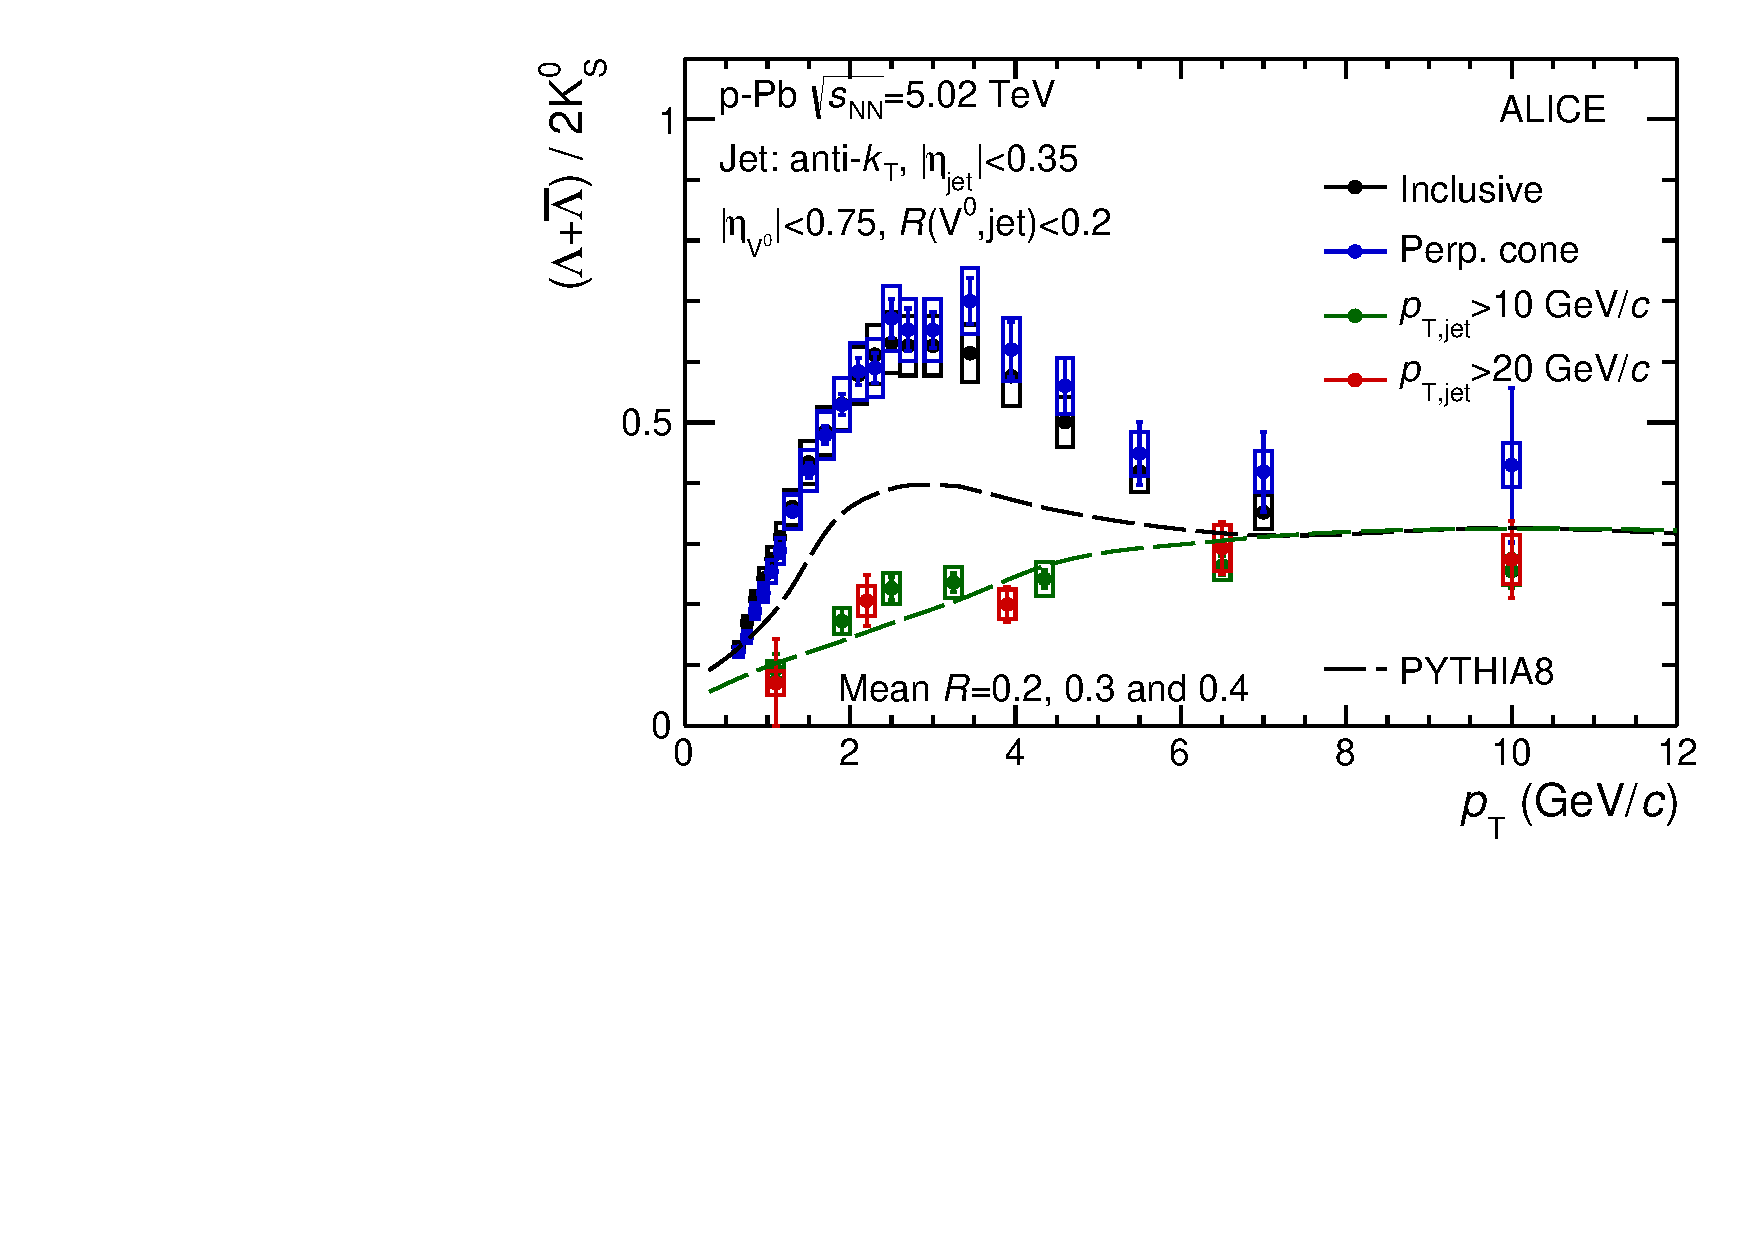
\includegraphics[width=0.49\textwidth]{cFig8a_pPb}
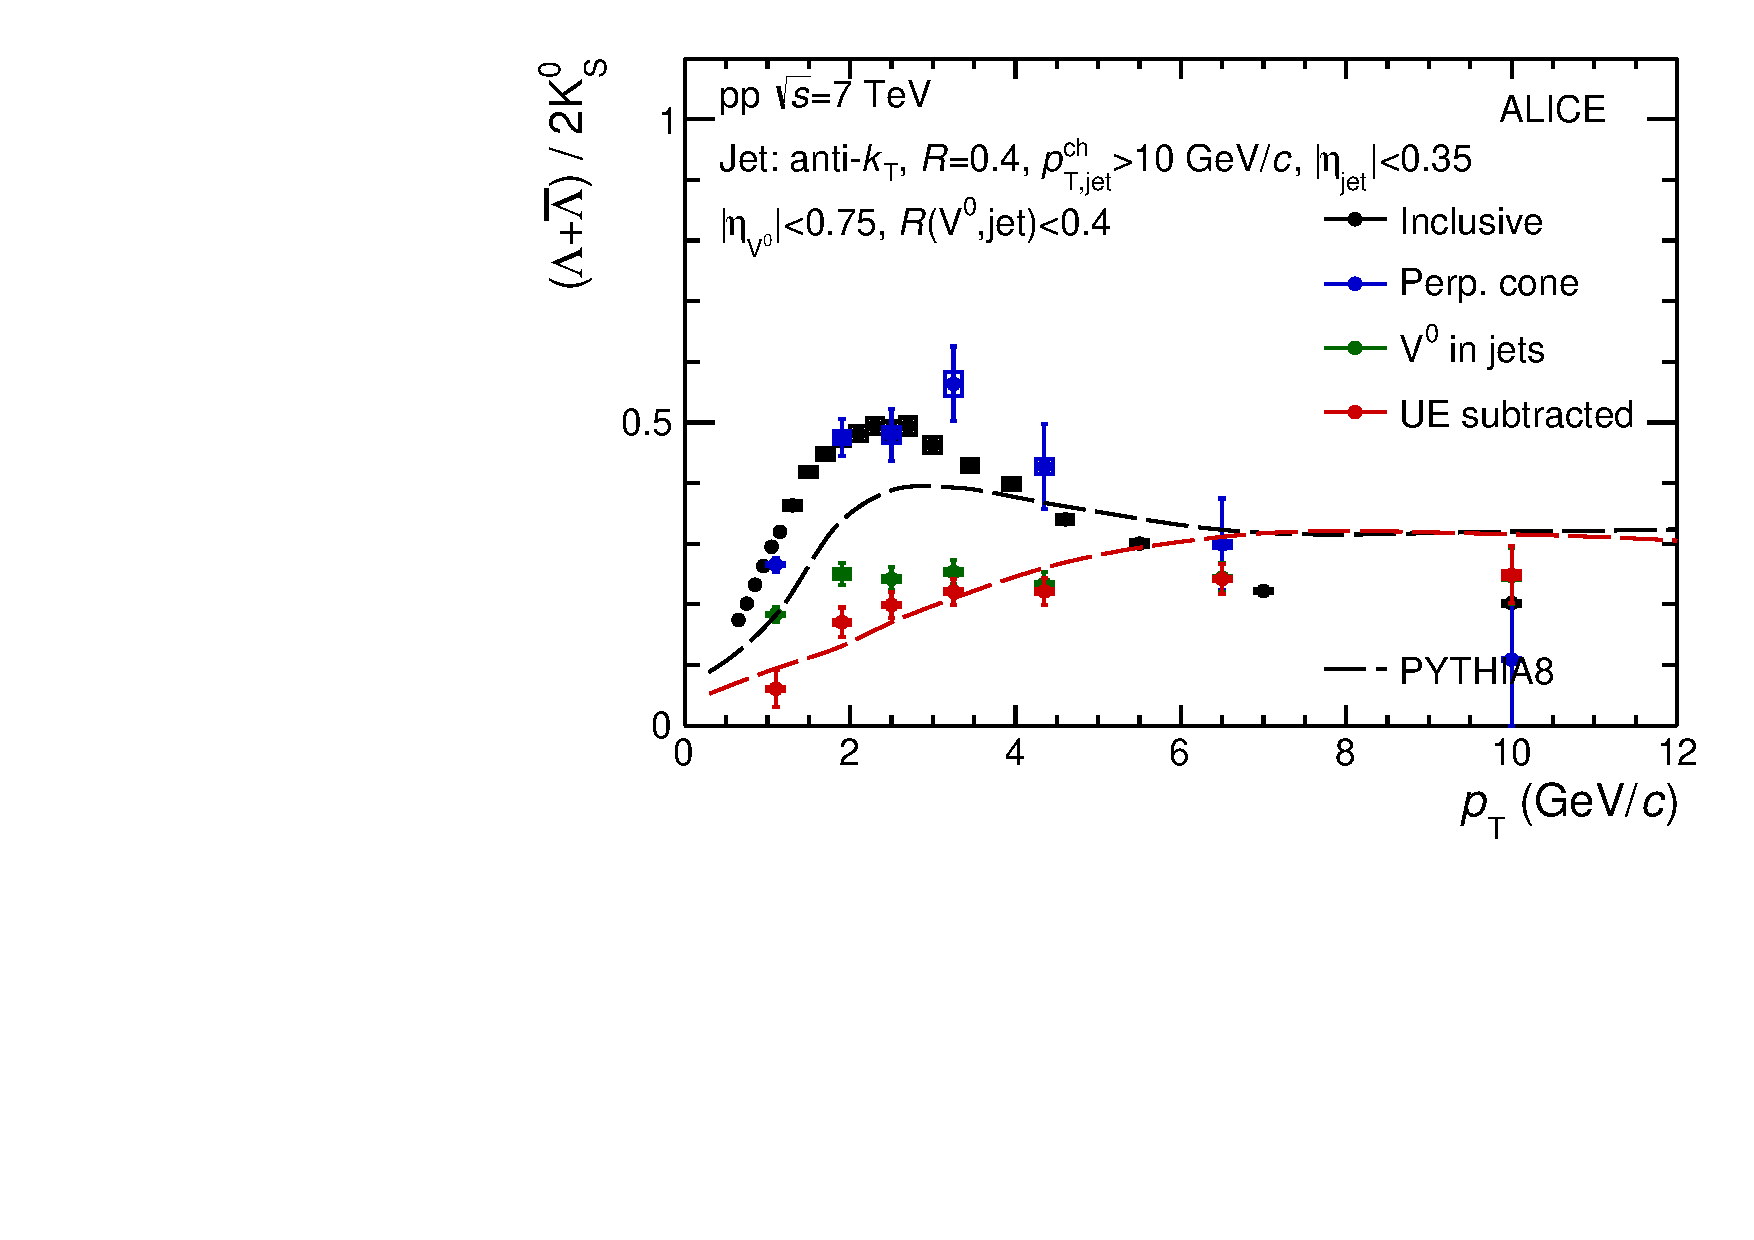
\includegraphics[width=0.49\textwidth]{cFig8b_pp}
\caption{\lda/\ks\ ratio in in \pPb\ collisions at \sqrtsnn{5.02} (left) \pp\ collisions at \sqrts{7} (right) as a function of \Vzero-particle \pt\ associated with charged jets with $\ptch>10~\gevc$ and $20~\gevc$ together with that in inclusive, PC distributions and JC selection in case of \pp\ collisions.}
	\label{fig:L2Kratio_pp_pPb}
\end{figure}

Selecting hard scatterings according to the jet energy carried exclusively by the primary charged particles induces biases and inefficiencies in selection of the parton showers.
The bias is related to the probabilistic process of fragmentation and hadronization.
The analysis presented here tags only parton showers fragmenting into a configuration of hadrons that produce a charged particle jet with $\ptch>10~\gevc$ with a given $R$ with a finite efficiency.
Therefore, there can be cases of \Vzero\ particles that originated from a parton shower but were rejected in the analysis based on the energy carried only by the primary charged particles.
The same analysis performed using the \pythia\ event generator shows that the most probable \pt\ of the full jet with $R=0.4$ is larger by about 40\% as compared to the \ptch.
Moreover, since the daughters of the \Vzero\ particles are not included in the jet energy calculation there are cases of jets containing \Vzero\ particles but not included in the JC selection.
On the other hand, Fig.~\ref{fig:L2Kratio_pp_pPb} shows that the inclusive \lda/\ks\ ratio at high-\pt\ is fully consistent with the ratio from particles associated to jets in this analysis. This suggests that the conclusion on the absence of the baryon/meson enhancement in jets made with the charged jets alone holds for all energetic parton showers and hadron configurations within the jets.
%%%%%%%%%%%%%%%%%%%%%%%%%%%%%%%%%%%%%%%%%%%%%%%%%%%%%%%%%%%%%%%%%%%%%

\begin{figure}[!t]
\centering
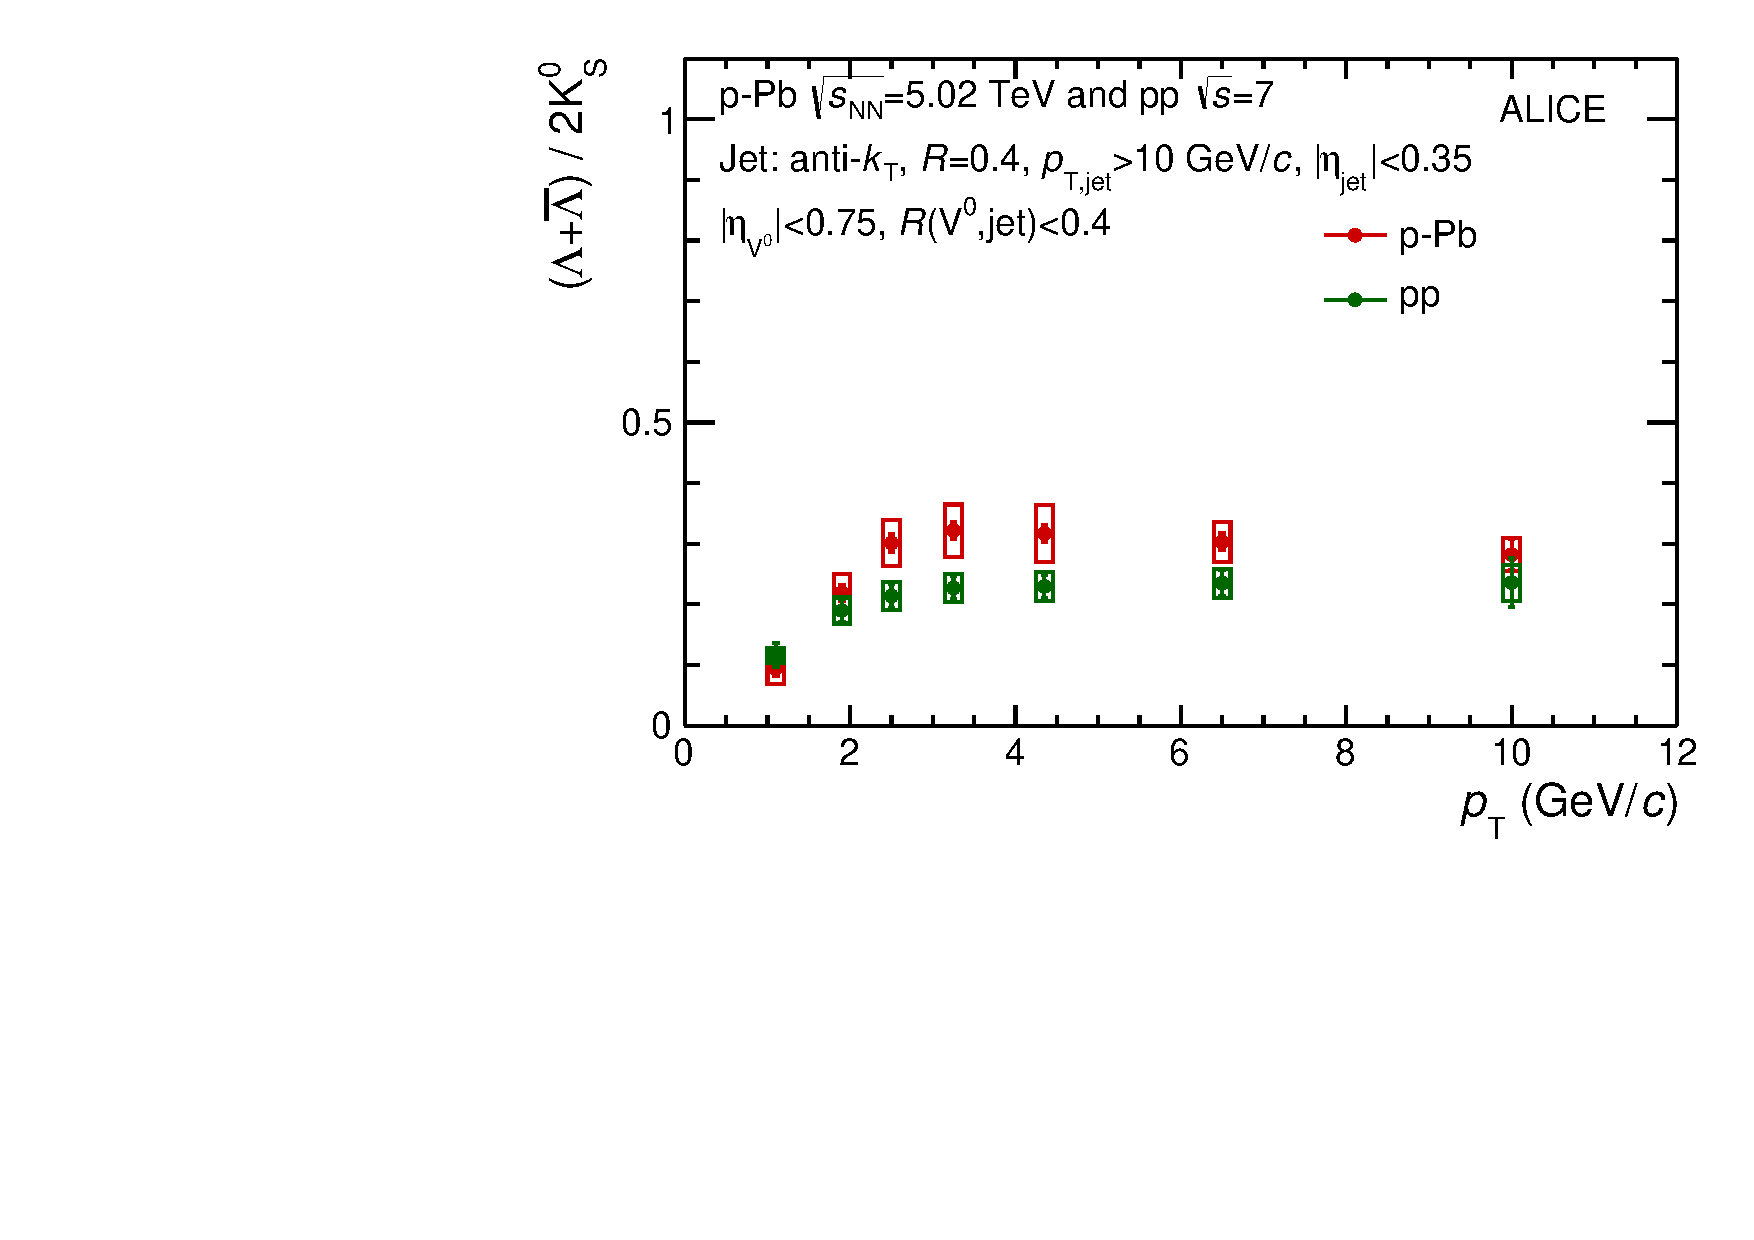
\includegraphics[width=0.80\textwidth]{cFig9}
\caption{\lda/\ks\ ratio in \pp\ collisions at \sqrts{7} and in \pPb\  collisions at \sqrtsnn{5.02} as a function of \Vzero-particle \pt\ associated with charged particle jets with $\ptch>10~\gevc$ reconstructed using \akT\ jet finder with resolution parameter $R=0.4$. The ratio is shown for the same selection of the matching radius $\rvzerojet<0.4$ in both systems.}
\label{fig:L2Kratio_pp_pPb_comparison}
\end{figure}

%% \subsection{Comparison to PYTHIA}

Figure~\ref{fig:L2Kratio_pp_pPb} shows a comparison to results obtained with the \pythia\ event generator run for proton--proton collisions at \sqrts{5.02} (left panel) and \sqrts{7} (right panel).
The jet selection within \pythia\ was made using the generator level information with the \pt\ cut of $10$~\gevc.
We find that the characteristic maximum at intermediate \pt\ in the inclusive ratio is not reproduced by the generator.
However, for both collision systems the ratio within jets after the subtraction of the underlying event is consistent with the data.
Note, \pythia\ has been chosen here as an example and we do not aim for a thorough review of the strangeness production in the Monte-Carlo generators.
We find the comparison with experimental data sufficient to demonstrate the clear similarities of the meson-to-baryon ratio within jets.
Figure~\ref{fig:L2Kratio_pp_pPb_comparison} shows the comparison of the ratio obtained in jets in \pp\ and \pPb\ collisions for the same selection of the matching radius $\rvzerojet<0.4$ in both systems.
The ratio obtained in \pPb\ collisions shows a small enhancement for $2<\pT<8~\GeVc$ with respect to that in \pp\ collisions.

\section{Summary}

In conclusion, the enhancement in the $(\lda+\alda)/\ks$ ratio found in the inclusive particle measurements in \pPb\ and \PbPb\ collisions is not present for particles associated to hard scatterings tagged by jets reconstructed from charged particles for $\ptch>10~\gevc$ in \pPb\ and \pp\ collisions.
%This unmodified ratio in \pPb\ as compared to \pp\ collisions is consistent with the measurements in \PbPb\ collisions \cite{Abelev:2013xaa,Abelev:2014laa,Adam:2015kca}.
Moreover, as the baryon/meson enhancement has been linked to the interplay of radial flow and parton recombination at intermediate-\pt\ its absence within the jet cone demonstrates that these effects are limited to the soft particle production processes.
